\documentclass[12pt]{report}
\usepackage{polyglossia}
\setdefaultlanguage{czech}


\usepackage{graphicx} % Required for inserting images

\usepackage{setspace}
\setstretch{1.15}
\usepackage{geometry}

\usepackage{fontspec}
\setmainfont{Times New Roman}
\setsansfont{Arial}

\usepackage{titlesec}

\usepackage{listings}
\usepackage{xcolor}
\usepackage{url}
\usepackage[backend=bibtex,style=numeric,sorting=none]{biblatex}
\usepackage{microtype}

\setlength{\emergencystretch}{3em}

\makeatletter
\patchcmd{\blx@theformat@labelnumber}{\the\value{instcount}}{\arabic{instcount}}{}{}
\makeatother
\addbibresource{Zdroje.bib}
\DeclareLanguageMapping{czech}{czech}
\usepackage{hyperref}

\hypersetup{
    colorlinks=true,
    linkcolor=blue,
    filecolor=magenta,
    urlcolor=cyan,
    pdftitle={\@title},
    pdfpagemode=UseNone,
}

\lstset{
    basicstyle=\ttfamily\small,
    numbers=left,
    numberstyle=\tiny,
    numbersep=5pt,
    tabsize=4,
    frame=none,
    breaklines=true,
    language=C,
    captionpos=b,
}
\gappto\captionsczech{%
  \def\lstlistingname{Kód}%
  \def\lstlistlistingname{Seznam kódů}%
}
\DefineBibliographyStrings{czech}{
  bibliography = {Seznam použitých zdrojů},
  url = {Dostupné z},
  and = {a},
}
\DefineBibliographyExtras{czech}{\def\urldateformat{czech}}
\DeclareFieldFormat{url}{\bibstring{url}\addcolon\space\url{#1}}

\DeclareFieldFormat[misc]{title}{\emph{#1}}
\DeclareFieldFormat[misc]{note}{Online.\addspace In: \emph{#1}\adddot}

\defbibheading{czech bibliography}[\bibname]{%
  \chapter*{Seznam použitých zdrojů}%
  \addcontentsline{toc}{chapter}{Seznam použitých zdrojů}%
}

\titleformat{\chapter}
  {\sffamily\textsixteen\bfseries}
  {\thechapter}
  {1em}
  {}
  
\titleformat{\section}
  {\sffamily\textfourteen\bfseries}
  {\thesection}
  {1em}
  {}

\titleformat{\subsection}
  {\sffamily\textthirteen\bfseries}
  {\thesubsection}
  {1em}
  {}

\titleformat{\paragraph}
  {\normalfont\normalsize\bfseries}
  {\theparagraph}
  {0.5em}
  {}

\titlespacing*{\paragraph}
  {0pt}
  {6pt}
  {6pt}

\makeatletter
\@addtoreset{paragraph}{subsubsection}
\makeatother
   
\titlespacing*{\chapter}
  {0pt}
  {0pt}
  {20pt}

\newcommand{\texttwenty}{\fontsize{20pt}{24pt}\selectfont}
\newcommand{\textsixteen}{\fontsize{16pt}{20pt}\selectfont}
\newcommand{\textfourteen}{\fontsize{14pt}{18pt}\selectfont}
\newcommand{\textthirteen}{\fontsize{13pt}{17pt}\selectfont}


\newgeometry{
    top=0.98in,
    bottom=0.98in,
    outer=0.98in,
    inner=0.98in,
}





\begin{document}

\begin{titlepage}
    \thispagestyle{empty}
    
    \begin{flushleft}
        
\includegraphics{img/0.png}

        \vspace{1.15in}

        {\sffamily \texttwenty \textbf{2D Videohra Salvation Path: Uživatelské rozhraní}\\}

        \vspace{10pt}
        
        {\sffamily \textfourteen 2D Video game Salvation Path: User interface\\}

        \vspace{40pt}
        
        {\sffamily \textsixteen Maturitní práce\\}
        {\sffamily \textsixteen Vedoucí práce: Bc. Adam Tyroň\\}
        {\sffamily \textsixteen 2025/26\\}
        {\sffamily \textsixteen Jonáš Kyml, 4.D\\}
    \end{flushleft}

\end{titlepage}

\section*{Abstrakt}
Tato práce se zabývá vývojem videohry \emph{Surreal Bowling: Salvation Path} a patří do skupiny tří maturitních prací ve třídě 4.D, které jsou na tuto videohru zaměřeny. Náš nezávislý tým se jmenuje \emph{Still Thinking Studio}. Všechny tři maturitní práce řeší z většiny programovací a logickou část toho, jak videohra funguje, avšak má práce se zaměřuje i na audiovizuální stránku této videohry, jelikož mám na starosti veškerý audio design, vizuální efekty a post-processing. Co se týče kódové části, věnuji se zejména uživatelskému rozhraní a logice, která odpovídá za správný chod událostí a různých managerů.

\section*{Klíčová slova}
videohra, 2D plošinovka, Unity, C\#

\section*{Abstract}
This thesis examines the development of the video game \emph{Surreal Bowling: Salvation Path} and is one of three graduation theses in class 4.D that focus on this particular video game. Our independent team is referred to as \emph{Still Thinking Studio}. The three graduation projects primarily address the programming and logical components of the video game's functionality. However, my own work also focuses on the audiovisual elements of the video game, as I am responsible for all audio design, visual effects, and post-processing. As for the coding part, the primary focus is on the user interface and the logic that is responsible for the proper functioning of events and various managers.

\section*{Key words}
video game, 2D platformer, Unity, C\#

\chapter*{Poděkování}
Rád bych poděkoval panu Bc. Adamu Tyroňovi za víceletou aktivitu na Discord serveru našeho vývojářského týmu a ujmutí se nás jako mentor maturitní práce. Dále chci samozřejmě poděkovat svým spolupracovníkům a zároveň spolužákům, s kterými videohry vyvíjím - Danielu Baierovi a Simeonu Bednarzovi za vyvíjení kódu a Jakubu Wojtasovi za téměř veškeré grafické zpracování.


\chapter*{Prohlášení}
Prohlašuji, že jsem svou maturitní práci vypracoval/a samostatně. K práci jsem použil/a literaturu a prameny, uvedené v seznamu. Souhlasím s tím, aby moje ročníková práce byla využívána na~Střední~průmyslové~škole~Karviná, příspěvkové organizaci.

\vspace{2\baselineskip}

\noindent V Karviné dne: ……………………….\hfill Podpis: ………………………. 

\tableofcontents

\chapter{Úvod}

Cílem práce je vyvinout základní komponenty uživatelského rozhraní videohry žánru 2D plošinovka, postarat se o správnou funkčnost game manageru, který se stará například o přepínání mezi jednotlivými scénami, audio manageru, jehož úkolem je přehrávat všechny zvukové efekty a OST ve správný čas správným způsobem, a jednotlivých UI elementů.

Dále se zabývá tvorbou vizuálních efektů, které jsou v herním průmyslu důležité pro zkrášlení grafické stránky a přidání jistého realismu do zážitku z prostředí videohry. Vizuální efekty pomáhají hráčům chápat systémy, rychleji registrovat, co se děje, dostávat pozitivní/negativní zpětnou vazbu a vtažení do děje.

Úzce s vizuálními efekty souvisí i zvukové efekty -- snad každý vizuální efekt může mít svůj korespondující zvukový efekt, který ještě více potlačí účinek celé specifické akce. Audio je mezi průměrnými hráči často přehlíženo, protože se bere jako samozřejmost vzhledem k tomu, že zvukové odezvy se v reálném světě odehrávají všude kolem nás. Zkuste si ale někdy vaši oblíbenou videohru zahrát kompletně bez zvuku -- potěšení z videohry v takovém případě u mnoha titulů může klesnout drasticky. Práce se tedy zaměřuje jak na zvukové efekty, tak i na hudební složku.

Nakonec je nastíněn i jednoduchý model postprocessingu, který grafice naší hry dodává atmosféru, aby se tolik nepodobala retro videohrám jako je například herní titul Super Mario Bros \cite{super-mario-bros}.
\chapter{Terminologie}

\section{GameObject}
Základní stavební prvek Unity enginu, reprezentující jakýkoli objekt ve scéně. To mohou být například postavy, budovy, zdroje světla, zdroje zvuku, textová pole nebo neviditelné objekty, které slouží čistě pro funkční účely (za pomoci skriptů připojených jako komponent na daný GameObject).

\section{OST}
Zkratka OST (Original Soundtrack) označuje hudební složku vytvořenou přímo pro daný film, seriál, videohru nebo jiné podobné médium.

\section{Post-processing}
Post-processing je proces aplikování vizuálních vylepšení, filtrů a posílení žádoucí atmosféry různými efekty. Mezi často používané efekty patří Color Grading, Bloom nebo Depth of Field.

\section{Singleton}
Singleton je návrhový vzor (design pattern) v objektově orientovaném programování, který zajišťuje, že daná třída má pouze jednu instanci a poskytuje globální přístup k této instanci. V kontextu Unity se singleton často používá pro manažery (například AudioManager nebo UIManager), kteří musí být přístupní z jakéhokoli místa v kódu a zároveň musí existovat pouze v jediné instanci. Singleton se typicky implementuje pomocí statické vlastnosti Instance a privátního konstruktoru, případně pomocí metody DontDestroyOnLoad pro perzistenci mezi scénami.

\section{Unity Editor}
Rozhraní Unity enginu, ve kterém se pracuje většinu času při vývoji videohry (podobně jako kreativní programy Blender, DaVinci Resolve nebo FL Studio).
\chapter{Použitý framework aplikace}

\section{Operační systém}
V týmu je jako hlavní operační systém pro vývoj hry \emph{Surreal Bowling: Salvation Path} používán operační systém Linux. Bylo tak rozhodnuto, jelikož nabízí rychlejší workflow než Windows. Během práce také bylo zjištěno, že pokud na Unity pracují dva vývojáři, jeden na Linuxu a druhý na Windows, stává se, že se některé soubory v Unity projektu stanou poškozené. Vývoj videoher v operačním systému Linux je dnes proveditelný a programy jako Unity Engine, VS Code nebo Git fungují stejně dobře, ne-li lépe, než na Windows. \cite{linux-gamedev}

\section{Programování}

\subsection{C\#}
Pro psaní kódu byl použit multiplatformní programovací jazyk C\#, mimo jiné i nejpopulárnější jazyk pro .NET. \cite{csharp} Více o C\# v části \ref{sec:herni-engine}.

\subsection{Textový editor}
Co se textového editoru týče, byl použit VS Code z důvodu kompatibility s nejvíce pluginy třetích stran. \cite{vscode-vs-codium}

\subsection{Version Control}
Pro spolupráci ve vývojářském týmu byl použit Git – systém pro správu verzí, neboli „version control system“ (VCS). Přes Git jsou posílány lokální změny do online repozitáře projektu na webovou platformu GitHub, kde má přístup i náš mentor práce, aby měl přehled o tom, jak se s vývojem vede. \cite{git-intro} 

\subsection{AI (Umělá Inteligence)}
Pro usnadnění psaní kódu, provádění repetitivních úkolů nebo přesouvání větších objemů dat byly použity AI asistenty ChatGPT \cite{chatgpt} a Augment Code \cite{augment}. Později i lokální LLM (Large Language Model) v programu LM Studio \cite{lmstudio} (konkrétně qwen/qwen3.5-9b \cite{qwen}) integrovaný do nástroje OpenCode \cite{opencode}, což umožnilo daný model používat jako agenta v terminálu, který dokáže indexovat celé projekty a provádět v nich úpravy.

\section{Herní engine}
\label{sec:herni-engine}
Jakožto nejdůležitější software pro vývoj videohry dnes je herní engine. Pro tento projekt byl zvolen multiplatformní herní engine Unity vyvinutý společností Unity Technologies \cite{unity} z několika prostých důvodů. Jeden z nejhlavnějších je ten, že v Unity se defaultně programuje v programovacím jazyce C\#.

Dále byly také brány v potaz licence různých herních enginů. Mezi nejznámější patří právě Unity, Unreal Engine, Godot Engine nebo GameMaker. Unity prozatím stačilo jako nejrozumnější cesta, kde je možné videohry vydávat pod Unity Free License \cite{unity-pricing}, pokud jednotlivec nebo tým z výdělku z videohry nebo od sponzora přijímá méně než 200 000 amerických dolarů za posledních 12 měsíců. Jedna z největších nevýhod je, že při startu zadarmo vyvinuté videohry v Unity se při startu videohry objeví úvodní obrazovka (splash screen) s nápisem „Made with Unity“, což pro účely této práce zas tak nevadí.

Videohra vyvíjena v této práci také není nijak složitá v porovnání s dnešním videoherním standardem a Unity se obecně považuje jako příjemnější volba pro menší projekty \cite{unity-small-projects}, jako mohou být mobilní aplikace nebo právě jednoduché 2D projekty.

\section{Hudba a zvuk}

\subsection{FL Studio}
Pro tvorbu hudby a zvukových efektů byl použit program FL Studio.

FL Studio je software (Digital Audio Workstation) pro skládání, produkci a mix hudby za pomocí digitálních nástrojů, pluginů, samplů a MIDI signálů.

Mezi pluginy třetích stran, které byly frekventovaně používány pro tvorbu či modifikaci zvuku, patří LABS \cite{labs}, FLEX \cite{flex}, Sytrus \cite{sytrus} a Deelay \cite{deelay}. Plugin Deelay využívám především pro jeho pokročilé možnosti filtrace, časové a výškové modifikace a efekty jako Chamber nebo vrstvené komplexní delaye, které dodávají zvukům glitcheovou, zkorumpovanou atmosféru. \cite{flstudio}

\subsection{FMOD Studio}
\label{sec:fmod-studio}
Původně byly pro implementaci zvuku do této hry používány low-level nástroje přímo od Unity, například AudioSource, AudioListener a AudioMixer.

Později bylo implementováno FMOD Studio -- profesionální nástroj (audio middleware) pro úpravu a implementaci zvuku do videoher, vyvinutý společností Firelight Technologies \cite{fmod}. FMOD Studio umožňuje sound designerům vytvářet komplexní zvukové systémy pomocí přívětivého rozhraní bez nutnosti složitého programování, zatímco vývojáři mohou tyto zvuky snadno propojit s kódem pomocí Unity integrace. FMOD studio nabízí pokročilé funkce jako pocit 3D prostoru, automatizace zvuku nebo nejrůznější zvukové efekty (např. reverb).

\section{Ostatní}
Pro efektivní spolupráci v týmu je používán poznámkový software Obsidian \cite{obsidian}, kde předplatné Obsidian Sync zefektivňuje práci jak každodenně, tak například i na game jamech. Toto předplatné umožňuje ve stejný čas přistupovat ke všem informacím, nápadům, řešením, skriptům a zapisovat nové, aniž by bylo třeba cokoli manuálně přeposílat přes komunikační médium.

Pro komunikaci je v týmu používána platforma Discord \cite{discord} v založeném serveru pod názvem \emph{Still Thinking Studio}, na kterém jsou všichni členové týmu i spolupracující zvenčí. Discord umožňuje psát si jako v každé běžné chatovací aplikaci, spravovat desítky různých textových a hovorových kanálů (oprávnění, přístup, kategorie…) a rychle si posílat obrázky, zvukové soubory nebo videa pro nápady a zpětnou vazbu od ostatních členů týmu.
\chapter{Celková koncepce řešení}

\section{Game Manager}
Videohry se obvykle skládají z různých scén, které mohou představovat jednotlivé levely, tutorial část, hlavní menu nebo závěrečné titulky. Kdyby videohry musely načítat všechny tyto scény najednou, zabralo by to zbytečně moc času a výpočetní síly i přesto, že se hráč nachází jen na jednom z těchto míst. To je jeden z příkladů optimalizace a logiky, které jsou klíčové pro plynulý chod videohry. Pro tyto účely je jsou používány objekty typu \emph{Game Manager} (dále také „herní manažer“).

Herních manažerů se ve videoherních projektech vyskytuje hned několik a každý má na starosti odlišnou funkční část videohry: Game Manager (základ -- stará se o přepínání mezi scénami, správné zmrazení času, jednoduché uživatelské rozhraní…), Audio Manager (zajišťuje správný chod veškeré logiky zvuku   v prostředí hry nebo v UI), Cursor Manager (upravuje vlastnosti kurzoru počítače pro účely videohry) a další manažery, které nejsou zas tak časté, ale mohou se hodit pro konkrétní případy (Tutorial Manager, Collectible Manager, DontDestroyOnLoad, Death Manager).

Herní manažer je (zejména v Unity) tedy „empty GameObject“ ve scéně, který má na sobě připojený stejnojmenný skript jako komponent, do kterého můžeme přidávat reference k dalším objektům ve scéně nebo v projektu (tělo hráče, další scéna, textové pole) a upravovat jakékoli parametry tohoto skriptu, které zpřístupníme Unity Editoru.

\section{Umírání}
Videohra je navrnuta tak, že každý level má dvě části: \emph{The Chase} a \emph{The Exploration}. V \emph{The Chase} je hráč naháněn masivní bowlingovou koulí, která, pokud hráče dožene a přejede ho, tím ho i zabije a hráč bude muset začít znovu. Toto je způsob smrti \emph{hard death}, kdy se po zabití hráče znovu načte celý level, všechny parametry se restartují a hráč si tak musí \emph{The Chase} zapamatovat celou nazpaměť včetně všech překážek.

\emph{The Exploration} využívá více milosrdnou \emph{soft death}, kdy, pokud hráč spadne nebo se mu nějak jinak povede zemřít, místo toho, aby se scéna načetla od začátku, tak je hráč jen přemístěn k poslednímu aktivovanému checkpointu. Lze říct, že tato videohra tak používá hybridní systém smrti.

\subsection{Checkpoint System}
Do této videohry je dobrý nápad zakomponovat \emph{Checkpoint System}, který zajistí, že pokud hráč bude umírat v pozdějších fázích daného levelu, nemusí celým levelem procházet znova, ale hra ho transportuje k nejbližšímu checkpointu, který si uložil.

Některé hry používají i auto-save systém, kdy hra ukládá progres skoro každým momentem, tudíž kdykoli videohru můžete vypnout, zapnout a objevit se na tom samém místě, kde jste hru opustili, avšak to je ideálnější spíš pro videohry žánru open-world a v této videohře bude stačit, pokud hráč bude docházet k checkpointům a aktivovat je.

\section{Emotion System}
Pro zpestření herního zážitku této videohry byl vymyšlen koncept \emph{Emotion System}. Hráč bude muset v části \emph{The Exploration} sbírat \emph{Conversation~Fragments} (úlomky konverzace), které obsahují atributy emocí, a na základě kontextu celé konverzace bude hráč muset správně určit, jestli má daný \emph{Conversation~Fragment} pozitivní, negativní, nebo neutrální emoci. Podle toho pak bude potřeba sesbírané \emph{Conversation~Fragments} správně umístit na \emph{The Altar} (oltář), který je schopen aktivovat portál do dalšího levelu v případě správné kombinace.

Díky tomuto konceptu videohra bude obsahovat i mírný puzzle-solving a integraci příběhu, které posílí atmosféru surrealismu, kterého videohra má docílit. Je totiž důležité, aby videohra neobsahovala pouze akci, ale i části, kde si hráč může oddechnout a připravit se na další akci. Stejně jako v hudbě, kde je komplikované mít majestátní, hlasité momenty, pokud není správně zacházeno s tichem. Vše je o kontrastu.

\section{UI}
Velkou kapitolou, která musí být v nějakém měřítku v každé videohře, je uživatelské rozhraní (dále také anglická zkratka UI). Jakákoli tlačítka, nastavení herního zážitku nebo interakce se světem videohry musí projít přes skripty, které řeší uživatelské rozhraní.

Jedna z nejzákladnějších částí UI je Input System, který řeší, jaké hardware vstupy způsobují jakou akci ve videohře. Dvě základní vstupní zařízení, kterými dnešní počítače disponují, jsou klávesnice a myš. Některé videohry používají pouze klávesnici (Hollow Knight od studia Team Cherry \cite{hollow-knight}) a některé zas pouze myš (Happy Game od studia Amanita Design \cite{happy-game}). Častěji se však můžete setkat s kombinací obou. Dříve byla ve vývoji této videohry používána kombinace obou -- levá ruka obsluhovala veškerý pohyb včetně skákání a dashe (rychlý posun kupředu), zatímco pravá ruka zaujímala pozici na myši, která byla využívána pro míření, střílení a „camera peeking". Postupem času se v projektu však přešlo výhradně na klávesnici, jelikož tato varianta lépe rozloží aktivitu mezi obě ruce a eliminuje potřebu přesunu ruky mezi zařízeními. V budoucnu je zvažována implementace více možností ovládání, aby si každý hráč mohl vybrat variantu, která mu nejvíce vyhovuje.

Poté, co videohra ví, jaké vstupy mají jaký učel, je třeba s těmito signály pracovat a používat je pro kontroly, mechaniky a orientaci v programu videohry. Nejčastější případ UI jsou panely, které mají různé účely. Například Pause Panel je lišta, která se objeví při pozastavení hry (nejčastěji stisknutím klávesy Escape), kde se mohou objevovat informace o aktuálním stavu hráče, nastavení hlasitosti zvuku nebo možnosti opuštění levelu a ukončení hry.

Dokonce hned první věc, kterou hráč po zapnutí videohry vidí, je nejčastěji obrazovka hlavního menu, která se ve většině případech skládá pouze z UI komponentů. Častá jsou tlačítka „Hrát“, „Nastavení“, „Ukončit“ a „Titulky“ s pozadím, názvem herního titulu a Main Menu hudbou hrající na pozadí.

\section{Vizuální efekty}
Vizuální efekty by, jako každá část, měly podpořit uvěřitelnost digitálního světa a angažovanost do něj. Neměly by na sebe lákat až moc pozornosti, pokud tak vyloženě nechceme. Příklady klasických vizuálních efektů ve hrách jsou:

\begin{itemize}
    \item efekt smrti (Death Screen) 
    \item impact effect (například dopad na zem, dash)
    \item glow effect (na hráči, aby viděl kolem sebe, nebo na jiných předmětech, aby byly rychle zaregistrovatelné)
\end{itemize}

Dosáhnout těchto efektů je možno různými způsoby: přidání prvků světla na určitý GameObject \cite{unity-point-light}, experimentování s Unity Particle System \cite{unity-particle-system} nebo manipulování určitývh prvků Post-processing.

\newpage

\section{Audio}

\subsection{OST}

Skládat hudbu pro hru je samozřejmě více kreativní postup, kdy její tvůrce může strávit hodiny sezením u hudebního nástroje nebo vybíráním či tvorbou ideálních zvuků, které má v hlavě. Hudba většinou podporuje již hotovou vizuální a příběhovou stránku videoher (nebo i filmů) -- málokdy se stává, že se svět videohry staví kolem hudby. Tato videohra má surreální, snovou a tajemnou atmosféru, jelikož sleduje příběh postavy, která hledá sebe sama, má neustálý strach, neví, co může čekat od nastávající chvíle, a chce se dostat do bezpečí. Během této cesty se potkává s nadpřirozenými jevy, které nedávají smysl a je v neustálém stavu zmatení.

Pro tato témata byly vybrány následující sonické elementy:

\begin{itemize}
    \item vzdušné, retro tóny inspirované interpretem Joe Hisaishim (populární japonský skladatel pro legendární filmy od Studio Ghibli) \cite{ghibli}, zejména skladbou „The Path of the Wind – Instrumental“\cite{hisaishi-path-wind}
    \item podivné reverb \& delay efekty
    \item mixolydický modus, dórský modus, ukrajinská dórská / rumunská mollová stupnice
    \item mikrotonální hudba, xenharmonie
    \item vinylový efekt
    \item Další inspirace byla převzata například ze skladeb „It’s Just a Burning Memory“ (The Caretaker) \cite{caretaker-burning-memory}, „Moog City 2“ (C418) \cite{c418-moog-city-2} nebo „Resonance“ (Home) \cite{home-resonance}.
\end{itemize}

\subsection{SFX}
SFX (sound effects), neboli zvukové efekty, jsou dnes brány už jako samozřejmost a lidé si tolik neuvědomují, kolik práce na pozadí odvádí. Tvorba zvukových efektů do videohry je tedy další velká část kreativní činnosti, kde je důležité představit si, jak celý svět zní, a vytvořit příslušný zvukový efekt pro každou věc, která by v reálném světě vydávala nějaký zvuk. Sem spadají ambience na pozadí (padání kapek v jeskyních, šumění listů ve vánku, šeptání lidí), zvuky konkrétních objektů / akcí (kroky, útok, aktivace portálu, sbírání předmětů, dopad na zem, simulace komunikace s ostatními postavami) a zvuky uživatelského rozhraní (zmáčknutí tlačítka, pozastavení hry, hover akce).

Zvukové efekty je tak možno rozdělit do dvou částí: diegetické a nediegetické. Diegetické jsou součástí prostředí hry, mohou je slyšet postavy ve hře, zatímco nediegetické jsou určené pro hráče, nespadají do prostředí hry a mají čistě funkční účely (zpětná vazba, indikátory…). V některých případech se v médiích používají i přechody mezi nediegetickými a diegetickými zvuky, které také mohou mít svůj význam. Můj oblíbený případ tohoto efektu je z televizního seriálu Arcane, kde je v první půlminutě této video ukázky slyšet, jak se hudba vycházející z balónu (prostředí světa) postupně přemění na podkladovou hudbu pro diváky.\footnote{Arcane: Season 2 | Ekko and Jinx Team Up (Nerd Clips HD). \url{https://youtu.be/B_KSH6w-gps}}

\section{Post-processing}
Post-processing dodává videohře atmosféru, šmrnc a oživuje její již zhotovenou grafickou stránku. Pracuje se světlem, stínováním, barvami, zrcadlením, šumem a dalšími efekty, které najdete ve většině grafických nástrojů. Tyto efekty jsou pak aplikovány jako poslední grafická vrstva, než obraz dojde na obrazovku, a mohou být zpřístupněny přes skripty a ovládány tak, aby reagovaly na události ve videohře. Mezi časté použití post-processingu patří:

\begin{itemize}
    \item práce s jasem (iluze fáze noci, realistické, intenzivní zesvětlení prostředí simulující explozi nukleární bomby…)
    \item saturace / desaturace obrazu pro vyzdvihnutí emocí
    \item VHS efekt pro videohry žánru „analogový horor“
\end{itemize}
\chapter{Popis aplikace}
\label{sec:popis-aplikace}

\section{Zpracování základního modelu hry}
\label{sec:zpracovani-zakladniho-modelu-hry}

\subsection{Struktura scén}
\label{sec:struktura-scen}

V Unity představují scény základní prostředí, ve kterých videohra operuje. Mohou to být například jednotlivé úrovně, avšak jejich využití je širší – mohou rovněž sloužit jako hlavní menu, nastavení, nebo jakékoliv jiné samostatné prostředí. V rámci této práce pracujeme se třemi základními scénami: \emph{MainMenu}, \emph{Level1} a \emph{Level2}.

První scénou, se kterou se hráč setká po spuštění aplikace, je hlavní menu (\emph{MainMenu}). To nabízí několik základních možností: vstup do herního prostředí, přizpůsobení nastavení nebo ukončení aplikace. Logiku k přechodu z menu do první úrovně řeším ve skriptu \texttt{UIManager.cs} pomocí metody \texttt{PlayGame()}, která využívá vestavěnou třídu \texttt{SceneManager}:

\begin{lstlisting}[caption={UIManager.PlayGame()}, label={lst:uimanager-playgame}]
using UnityEngine;
using UnityEngine.SceneManagement;

public class UIManager : MonoBehaviour
{
    private void PlayGame()
    {
        SceneManager.LoadScene("Level1");
    }
}
\end{lstlisting}

Pro práci se scénami v Unity je nutné nejprve přidat požadované scény do seznamu scén v tzv. \emph{Build Settings}. V Unity editoru se tento seznam nachází v menu File > Build Settings > Scene List. Scéna musí být před přidáním otevřena v editoru a následně přidána pomocí tlačítka \emph{Add Open Scenes}. Po přidání lze na scénu odkazovat buď pomocí jejího indexu v seznamu, nebo pomocí jejího názvu. Já preferuji odkazování názvem pro lepší čitelnost kódu.

Po úspěšném dokončení úrovně \emph{Level1} je hráč automaticky přesunut do \emph{Level2}. Z jakékoliv úrovně se hráč může vrátit do hlavního menu pozastavením hry a aktivací panelu \emph{Pause Menu}, což je podrobněji popsáno v podkapitole \ref{sec:ui-prvky}.

\subsection{Herní manažery}
\label{sec:herni-manazery}
Herní manažery představují klíčové komponenty architektury videohry, které řídí specifické herní systémy a zajišťují komunikaci mezi různými částmi aplikace. V aktuální verzi využívám tři hlavní manažery:
\begin{itemize}
    \item \emph{UI Manager}
    \item \emph{Audio Manager}
    \item \emph{Cursor Manager}
\end{itemize}

\emph{UI Manager} je zodpovědný za veškerou logiku související s uživatelským rozhraním. Kromě dříve zmíněného přepínání mezi scénami řeší aktivaci jednotlivých panelů (například pause menu nebo nastavení) a komunikaci s knihovnou UI Toolkit, která je podrobněji popsána v podkapitole \ref{sec:ui-toolkit}.

\emph{Audio Manager} spravuje zvukovou složku aplikace. Jeho úkolem je aktivace odpovídající hudby, zvuků vztahujících se k danému prostředí (ambience) a především komunikace s externím nástrojem FMOD Studio. Součástí \emph{Audio Manageru} je také objekt \emph{FMODEvents}, který propojuje konkrétní zvuky vytvořené v databázi FMOD Studio s rozhraním Unity editoru a zpřístupňuje jednotlivé zvukové soubory pro manipulaci v kódu.

\emph{Cursor Manager} je funkčně nejjednodušším manažerem v celé struktuře. Jeho jedinou funkcí je vizuální kontrola kurzoru myši ve hře. V aktuální implementaci jsou používány dva stavy: normální kurzor a kurzor při stisku tlačítka. Zde je ukázka základní struktury tohoto skriptu:

\begin{lstlisting}[caption={CursorManager.cs}, label={lst:CursorManager}, frame=none, backgroundcolor=\color{white}]
using UnityEngine;

public class CursorManager : MonoBehaviour
{
    [SerializeField] private Texture2D normalCursorTexture;
    [SerializeField] private Texture2D clickedCursorTexture;

    private bool isClicking = false;

    private void Update()
    {
        bool currentlyClicking = Input.GetMouseButton(0);
        
        if (currentlyClicking != isClicking)
        {
            isClicking = currentlyClicking;
            UpdateCursorSprite();
        }
    }

    private void UpdateCursorSprite()
    {
        Texture2D currentTexture = isClicking ? clickedCursorTexture : normalCursorTexture;
        
        if (currentTexture == null)
        {
            Cursor.SetCursor(null, Vector2.zero, CursorMode.Auto);
            return;
        }
        
        Cursor.SetCursor(currentTexture, Vector2.zero, CursorMode.Auto);
    }
}
\end{lstlisting}

Skript využívá metodu \texttt{DontDestroyOnLoad}, aby instance manažeru přetrvávala mezi scénami. V metodě \texttt{Update()} se každým snímkem kontroluje stav levého tlačítka myši – při změně stavu se zavolá \texttt{UpdateCursorSprite()}, která nastaví odpovídající texturu kurzoru.

Na Linuxu se mi vyskytly problémy se zpožděním kurzoru, proto skript obsahuje dodatečná složitější řešení z internetu, která na něm zajišťují lepší odezvu.

\subsection{Input systém}
\label{sec:input-system}

Input systém je jedním z více témat, ke kterému se dá přistupovat více způsoby. Můžeme ho řešit nízkoúrovňově, jako v tomto případě, kdy nasloucháme stisknutí kláves přímo pomocí C\#:

\begin{lstlisting}[caption={Nízkoúrovňové zpracování vstupu}, label={lst:low-level-input}]
if (Event.current.isKey)
{
    // klávesa, která byla stisknuta.
    KeyCode key = Event.current.keyCode;
}
\end{lstlisting}

Pro tento účel však existuje modernější systém, který zajišťuje mnohem přívětivější a flexibilnější workflow. Je jím \emph{Input System}, který je zobrazen na obrázku \ref{fig:unity-input-system}.

\begin{figure}[h!]
    \centering
    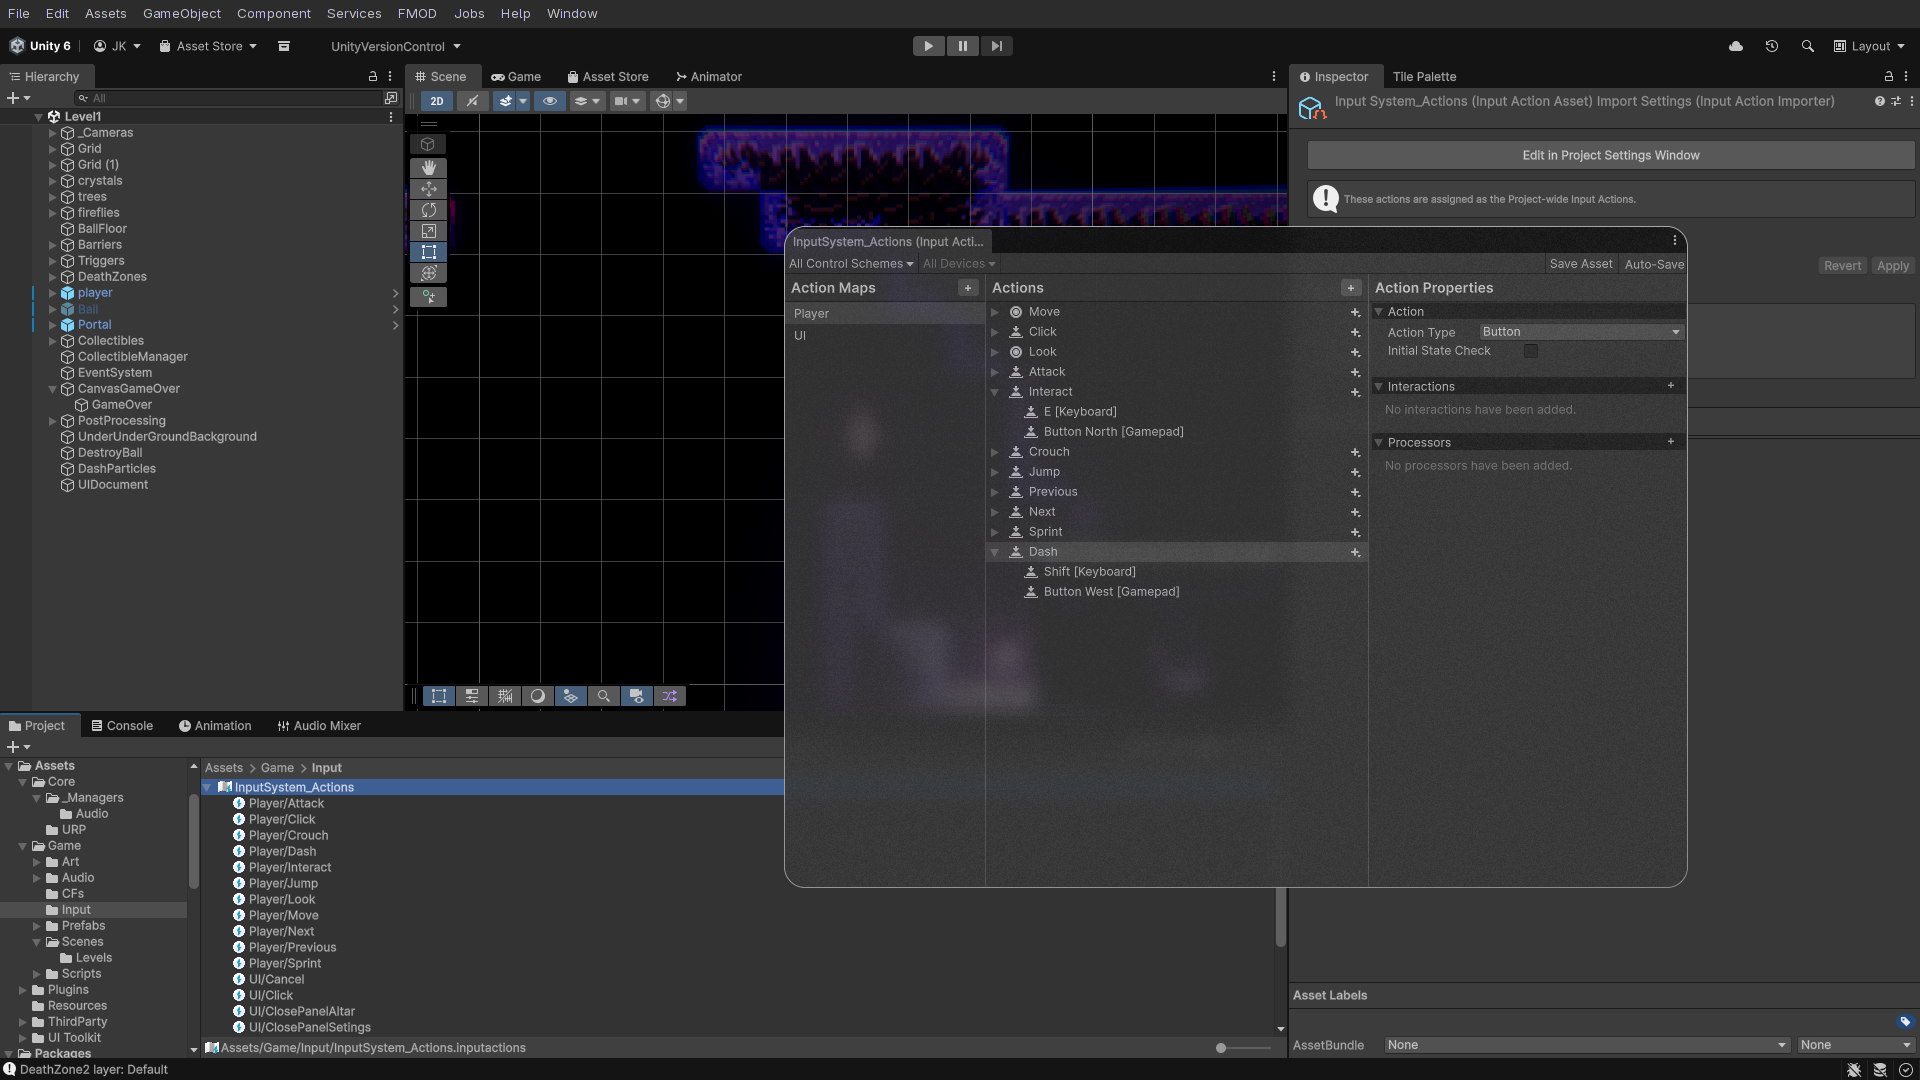
\includegraphics[width=1\textwidth]{img/unity/unity-input-actions.png}
    \caption{Rozhraní Unity Input System}
    \label{fig:unity-input-system}
\end{figure}

Jak můžeme vidět na obrázku \ref{fig:unity-input-system}, v tomto rozhraní můžeme vytvářet \emph{Action Maps} (vlevo). Naše videohra momentálně využívá dvě \emph{Action Maps}, jednu pro herní mechaniky a druhou pro orientaci v uživatelském rozhraní. Toto velmi usnadňuje řešení toho, jaké akce chceme od hráče vyžadovat.

Například jedním z nepříjemných problémů, které \emph{Action Maps} řeší, je následující: V minulosti, když jsem vstup řešil ještě zastaralým způsobem, UI fungovalo tak, že i když hráč pozastavil hru a dostal se do \emph{Pause Menu}, čas se zastavil – viz ukázka kódu \ref{lst:pause-code-old}.

\begin{lstlisting}[caption={Původní řešení pozastavení hry}, label={lst:pause-code-old}]
private void SetPauseState(bool pause)
{
    if (pauseMenu != null)
        pauseMenu.SetActive(pause);

    if (pause)
    {
        Time.timeScale = 0f;
        AudioManager.instance.PauseMusic();
    }
    else
    {
        Time.timeScale = 1f;
        AudioManager.instance.ResumeMusic();
    }
}
\end{lstlisting}

Toto řešení zastavilo veškerý pohyb ve hře. Všechny vstupní akce však zůstaly povolené a byly rozházené po projektu ve skriptech pro ovládání hráče, střelbu nebo animace. Proto, i přes zastavený čas, když hráč například spustil akci pro střelbu, i v \emph{Pause Menu} se hráči objevila střela u těla a hned jak hráč hru znovu spustil, střela odpalovala. Nebo pokud se hráč pokoušel hýbat v \emph{Pause Menu}, fyzicky se hýbat nemohl, ale animace fungovaly a hráč se tak mohl stále otáčet ze strany na stranu. To vypadalo neprofesionálně.

Za pomoci \emph{Action Maps} však složité ošetřování těchto chyb rychle mizí – viz ukázka \ref{lst:pause-code-new}.

\begin{lstlisting}[caption={Moderní řešení pozastavení pomocí Input System}, label={lst:pause-code-new}]
private void SetPauseState(bool pause)
{
    if (pause)
    {
        Time.timeScale = 0f;
        playerActionMap.actionMap.Disable();
        uiActionMap.actionMap.Enable();
    }
    else
    {
        Time.timeScale = 1f;
        uiActionMap.actionMap.Disable();
        playerActionMap.actionMap.Enable();
    }
}
\end{lstlisting}

Přes skript \texttt{UIManager.cs} mohu k \emph{Input Actions} souboru přistoupit a deaktivovat celou jednu \emph{Action Map}, která obsahuje jednotlivé \emph{Input Actions}. To znamená, že pokud hráč pozastaví hru a dostane se do \emph{Pause Menu}, mohu jednoduše zakázat \emph{Action Map} s názvem \emph{Player}, která obsahuje všechny možnosti ovládání herních mechanik, jako pohyb, speciální schopnosti nebo interakce se světem, a aktivovat \emph{Action Map} s názvem \emph{UI}, protože hráč se vskutku v daném momentu nachází v panelu uživatelského rozhraní, kde potřebuje pouze tyto \emph{Input Actions} včetně stisknutí klávesy \texttt{Esc}, která deaktivuje \emph{Pause Panel}, vrátí hráče do hry, deaktivuje \emph{Action Map} pro UI a aktivuje \emph{Action Map} pro ovládání hráče.

Napravo od sekce \emph{Action Maps} se nachází sekce \emph{Actions}, kde již nastavujeme konkrétní \emph{Input Actions}. Ve verzi pro tuto maturitní práci využívám pro \emph{Action Map} hráče následující akce:

\begin{itemize}
    \item \textbf{Move} -- pohyb (WASD / šipky)
    \item \textbf{Attack} -- střelba (K / Enter)
    \item \textbf{Interact} -- interakce s objekty (E)
    \item \textbf{Jump} -- skok (Space)
    \item \textbf{Dash} -- rychlý úskok (Shift)
    \item \textbf{Click} -- kliknutí myší pro střelbu
\end{itemize}

Pro \emph{Action Map} uživatelského rozhraní pak:

\begin{itemize}
    \item \textbf{Click / Point} -- kliknutí a pozice kurzoru myši
    \item \textbf{ScrollWheel} -- scrollování
    \item \textbf{TogglePause} -- pozastavení hry (Esc)
    \item \textbf{ClosePanelSettings / ClosePanelAltar} -- zavření nastavení nebo oltáře (Esc / E)
\end{itemize}

Ke každé \emph{Input Action} lze v sekci \emph{Action Properties} nastavit typ akce (\emph{Button}, \emph{PassThrough}, \emph{Value}), cílovou platformu (klávesnice, myš, herní ovladač, VR ovladač\dots) a případně další vlastnosti. Toto umožňuje multiplatformní nasazení na PC, macOS, PlayStation 5, Xbox Series X/S nebo VR headsety bez nutnosti měnit kód.




"
\subsection{Základní herní objekty}
\label{sec:zakladni-herni-objekty}

Mezi hlavní prvky ve scéně patří:

\textbf{Kamera} -- díky ní může hráč vidět, co se děje. S kamerou je možno dělat mnoho věcí, na které se podíváme později.

\textbf{GameObject hráče} -- objekt, na kterém je renderován sprite hráče a animace (viz obrázek \ref{fig:unity-gameobject-player}). Jsou na něm připnuty skripty jako \texttt{PlayerController.cs}, sloužící pro základní kontroly jako je pohyb, zvukový emitor atd. V naší hře je objekt hráče vždy na očích v oblasti středu okna aplikace.

\textbf{Uživatelské rozhraní} -- to může být řešeno více způsoby. Způsob, který najdeme ve většině tutoriálů, je \emph{Canvas} (viz podkapitola \ref{sec:ui-toolkit}). V hierarchii Unity se přidá GameObject Canvas a do něj lze přidávat jednotlivé UI elementy jako další objekty (tlačítka, slidery, panely, text).

Na již dříve zmíněném Brackeys Game Jam 2026.1 (viz podkapitola \ref{sec:fmod-studio}) jsem kromě jiného přišel k lepší alternativě i zde -- \emph{UI Toolkit}. Toto řešení vyžaduje mít ve scéně \emph{UI Document} (kde se řeší struktura) a \emph{UI Manager}, který s ním komunikuje a binduje k němu ostatní skripty.

Hierarchie scény je zobrazena na obrázku \ref{fig:unity-hierarchy} úplně vlevo.

\begin{figure}[h!]
    \centering
    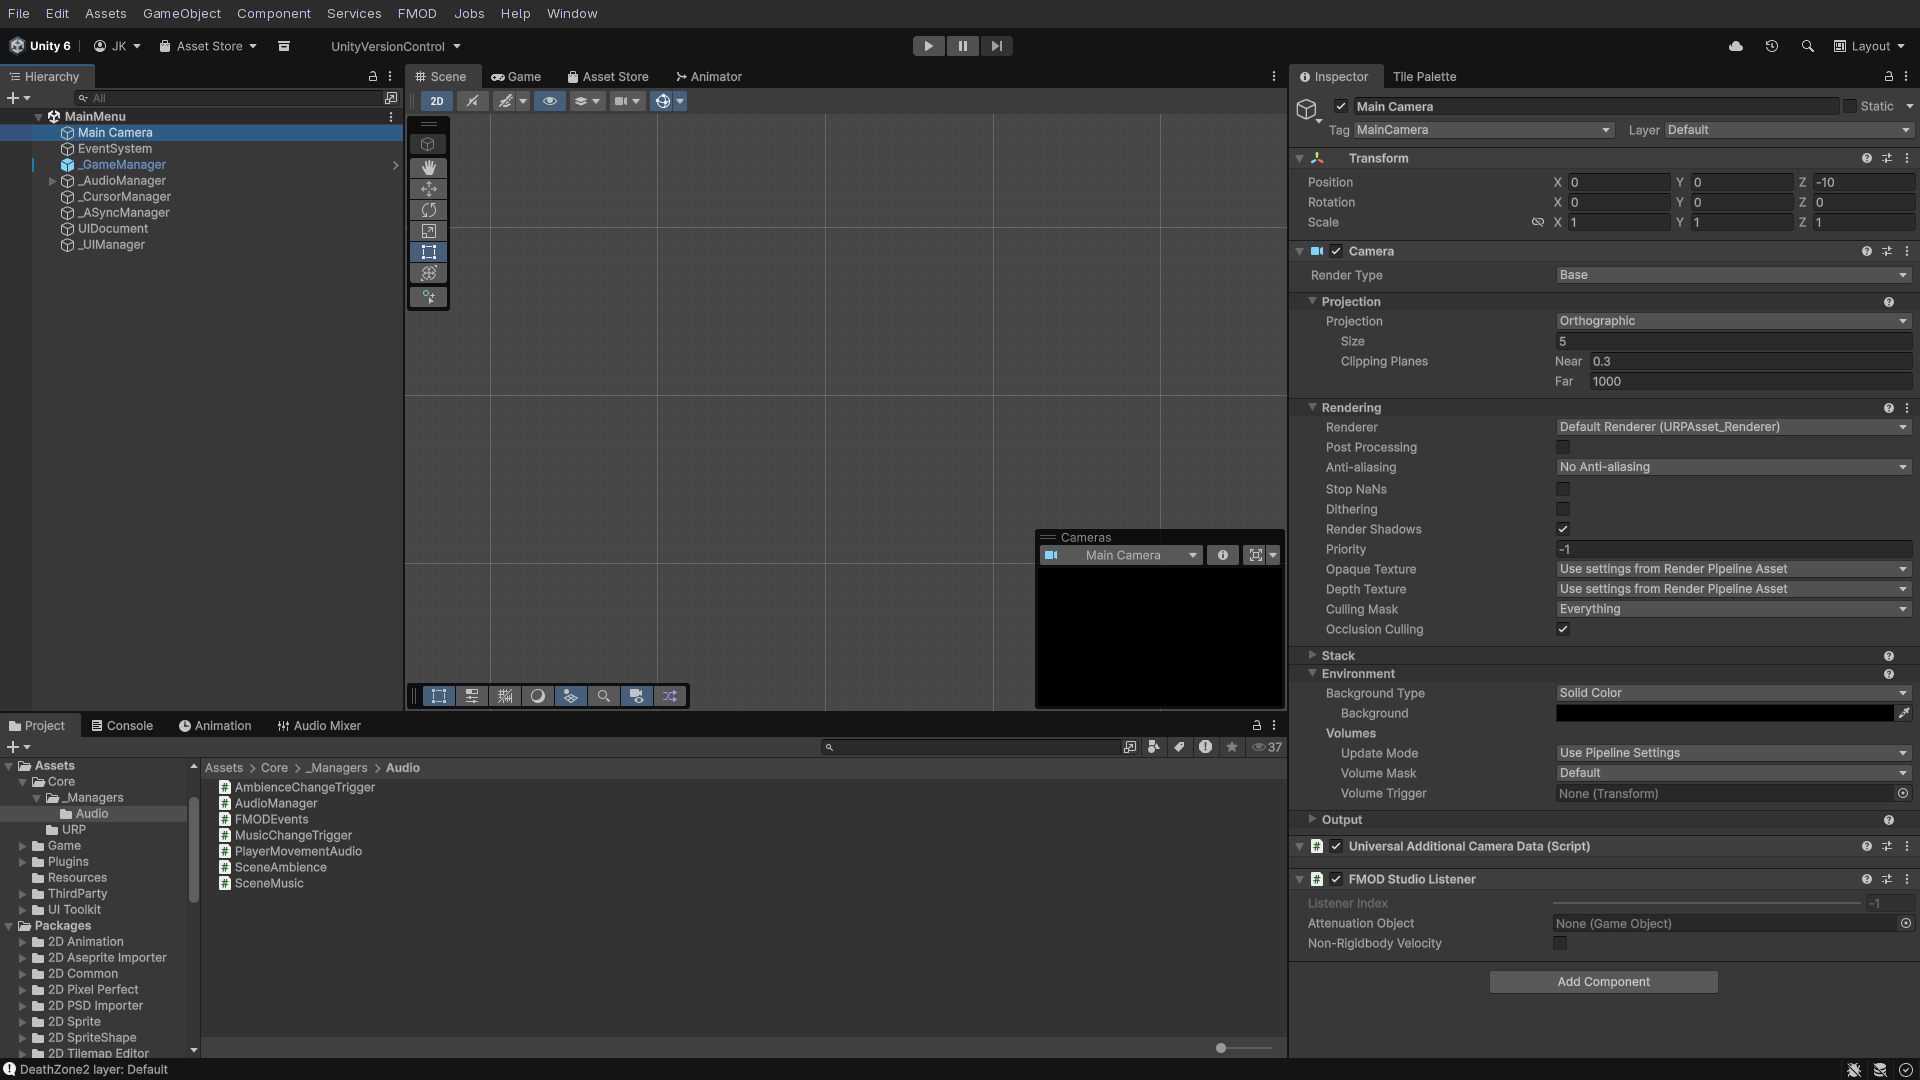
\includegraphics[width=1\textwidth]{img/unity/unity-hierarchy.png}
    \caption{Hierarchie scény}
    \label{fig:unity-hierarchy}
\end{figure}

\begin{figure}[h!]
    \centering
    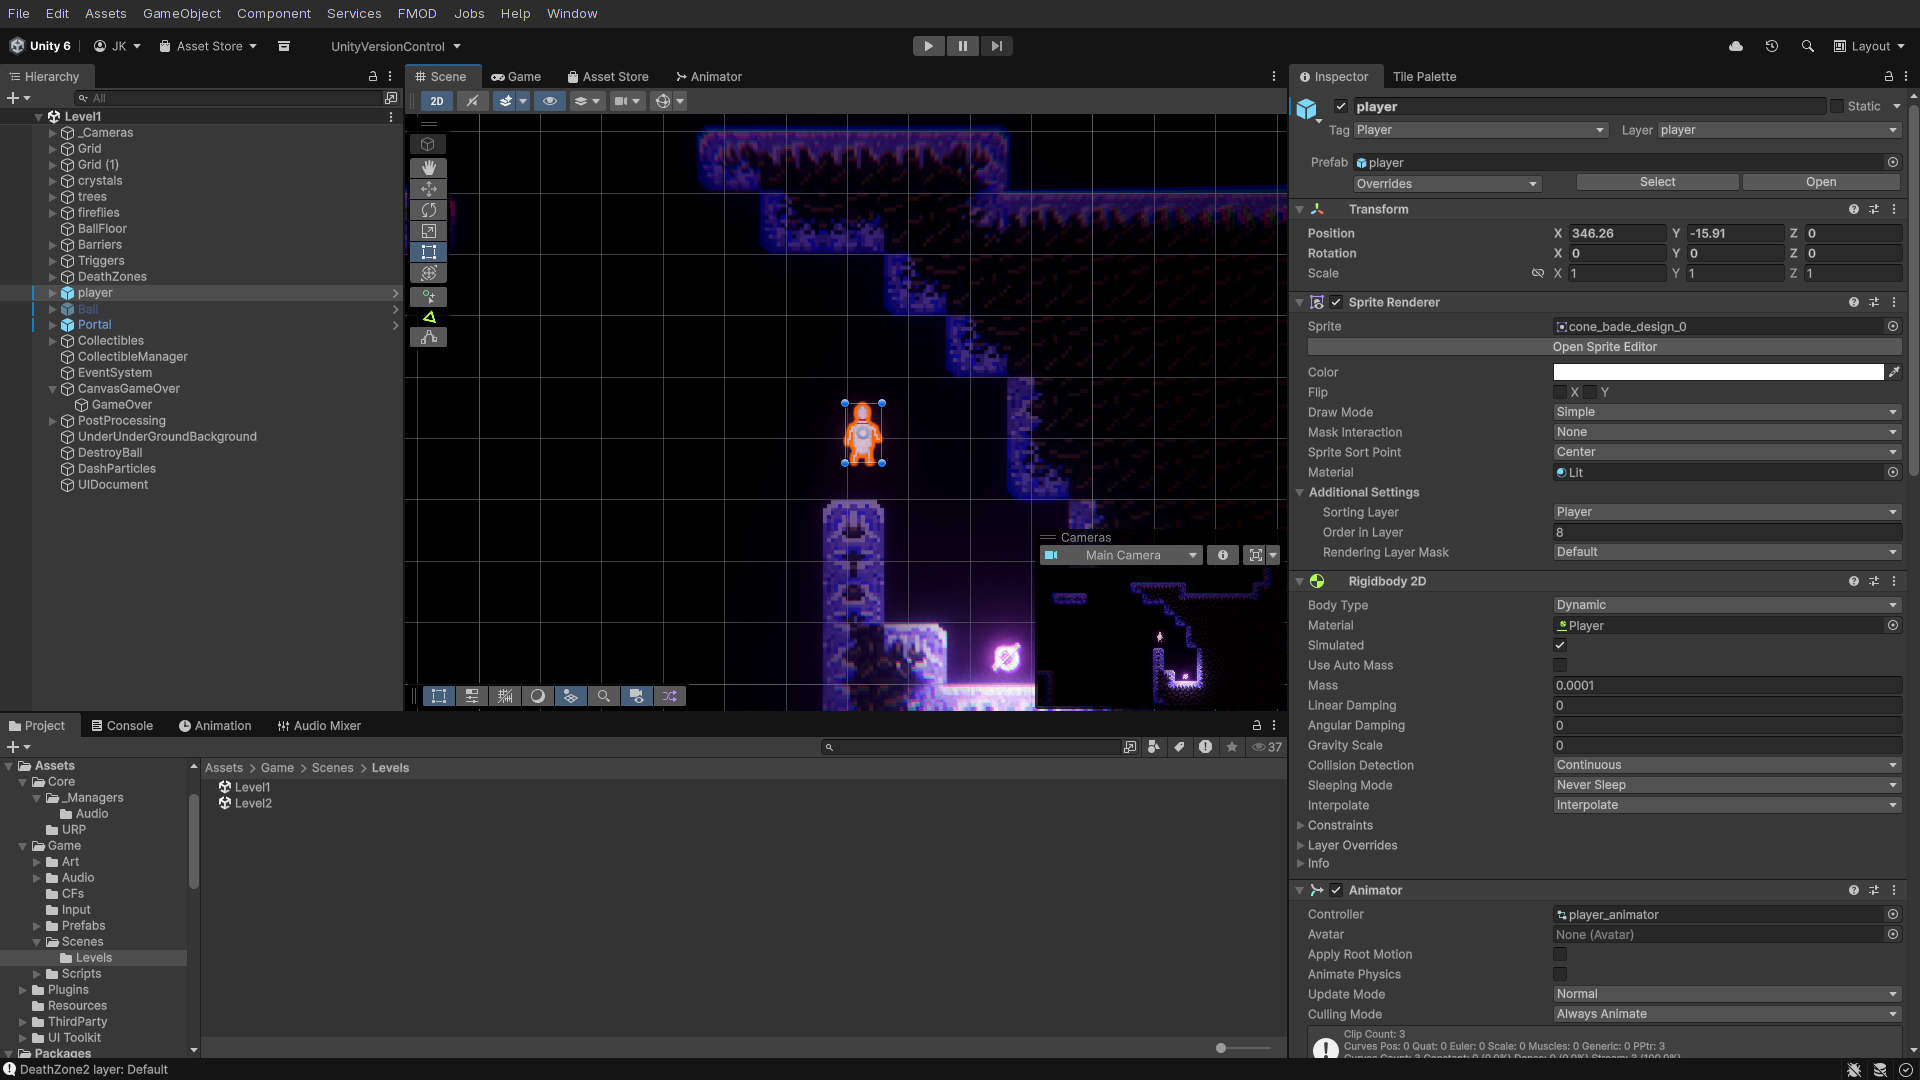
\includegraphics[width=1\textwidth]{img/unity/unity-gameobject-player.png}
    \caption{GameObject hráče ve scéně}
    \label{fig:unity-gameobject-player}
\end{figure}


\section{Vytvoření uživatelského rozhraní}
\label{sec:vytvoreni-uzivatelskeho-rozhrani}

\subsection{UI Toolkit}
\label{sec:ui-toolkit}

UI Toolkit je relativně novější způsob řešení uživatelského rozhraní než původní systém \emph{Canvas}. Od něj se liší například tím, že pro sestavení a stylizaci vizuálních elementů nepoužívá klasickou \emph{GameObject} strukturu, ale jazyky UXML (struktura) a USS (stylizace), které se svým provedením více podobají webovému vývoji.

Psát UXML nebo USS kód však vůbec není nutné. UI Toolkit má své grafické rozhraní, ve kterém je možné elementy přidávat myší a v inspektoru jim upravovat různé parametry jako pozici, velikost, margin, padding, velikost textu, barvu pozadí nebo jaký sprite by kurzor myši měl nad daným elementem zobrazovat. Toto grafické rozhraní je napojeno na \emph{UIDocument}, který ve scéně musí být také.

UI Toolkit však nepoužívá singleton logiku na \emph{UIDocument} -- ten není omezen na jednu scénu a je globální, podobně jako prefaby. Místo toho je singleton vzor aplikován na \emph{UIManager}, který drží reference na jednotlivé panely a spravuje jejich stav pomocí \emph{GameState} enumu. Tím se UI odděluje od datové vrstvy -- struktura UI je definována v UXML, zatímco logika je soustředěna v jednom centrálním skriptu.

Strukturu uživatelského rozhraní lze rozdělit na dvě hlavní kategorie: UI a HUD. UI je obecný pojem pro všechny elementy uživatelského rozhraní, se kterými hráč může interagovat -- tlačítka, inventář, textové oblasti dialogů. Naproti tomu HUD (Heads-Up Display) se skládá z elementů, které jsou perzistentně zobrazovány na obrazovce hráče během hraní -- ukazatel zdraví, počítadlo nábojů nebo malá mapa na kraji obrazovky.

Jak jsem postupně přecházel z \emph{Canvas} na UI Toolkit, mohl jsem porovnat obě řešení. Ve starších verzích bylo UI postaveno na principech:

\begin{itemize}
    \item Více samostatných \emph{Canvas} objektů ve scéně (např. \texttt{CanvasGameOver}, \texttt{Canvas HUD})
    \item Každý panel jako samostatný \emph{GameObject} s komponentami jako \texttt{Image}, \texttt{Button}, \texttt{Text}
    \item Skrývání a zobrazování panelů pomocí \texttt{GameObject.SetActive(true/false)}
    \item Rozptýlená logika mezi skripty jako \texttt{StripeCounterUI.cs}, \texttt{OrbCounterUI.cs}
\end{itemize}

S UI Toolkit v nejnovější verzi přichází zjednodušení:

\begin{itemize}
    \item Jeden \emph{UIDocument} definuje veškeré UI v jednom UXML souboru
    \item Všechny panely (MainMenu, PanelSettings, PanelPause, PanelAltar, HUD) jsou dotazovány pomocí \texttt{root.Q<VisualElement>("NazevPanelu")}
    \item Zobrazování pomocí \texttt{VisualElement.style.display = DisplayStyle.None/Flex}
    \item Centralizovaná správa stavu pomocí \texttt{GameState} enumu (None, Gameplay, Altar, Pause)
\end{itemize}

Rozhraní UI Toolkit je zobrazeno na obrázku \ref{fig:ui-toolkit}.

\begin{figure}[h!]
    \centering
    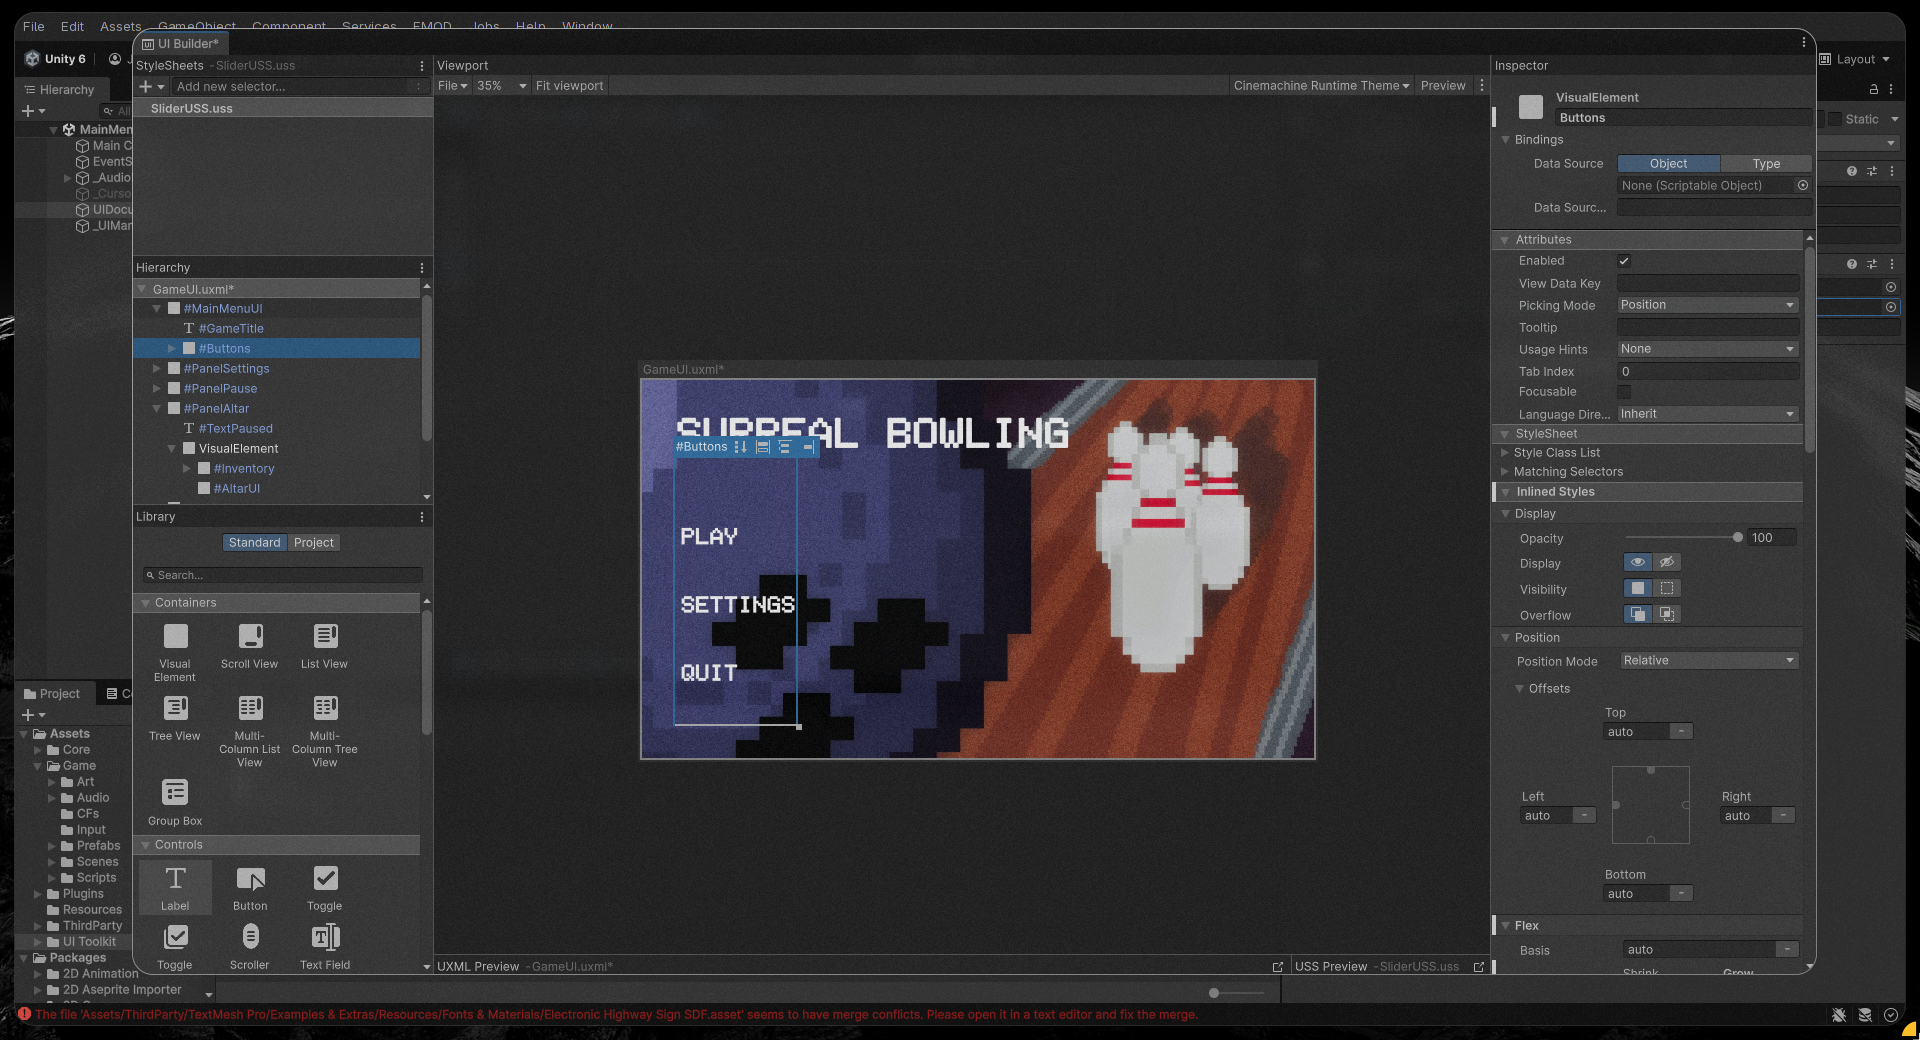
\includegraphics[width=1\textwidth]{img/unity/unity-ui-toolkit.png}
    \caption{Rozhraní UI Toolkit}
    \label{fig:ui-toolkit}
\end{figure}





\subsection{UI Prvky}
\label{sec:ui-prvky}

Na centrálním \emph{UIManageru} je postavena veškerá logika jednotlivých UI prvků. Každý prvek je definován v UXML souboru a následně bindován k odpovídajícím skriptům.

\textbf{Pause Menu} -- obsahuje tlačítko pro návrat do hlavního menu. Jeho řízení je součástí \texttt{GameState} systému, nikoliv pouze přes \texttt{Time.timeScale}. Metoda \texttt{SetState()} přepíná mezi stavy a při vstupu do \emph{Pause} zároveň aktivuje \emph{UI Action Map} a deaktivuje \emph{Player Action Map}, což je podrobně popsáno v podkapitole \ref{sec:input-system}. Přechod mezi stavy \emph{Gameplay}, \emph{Pause} a \emph{Altar} řeší jediná metoda:

\begin{lstlisting}[caption={UIManager -- přepínání stavů pomocí GameState enumu}, label={lst:uimanager-gamestate}]
void SetState(GameState newState)
{
    if (CurrentState == newState) return;
    CurrentState = newState;

    panelPause.style.display = DisplayStyle.None;
    panelAltar.style.display = DisplayStyle.None;
    HUD.style.display = DisplayStyle.None;

    switch (newState)
    {
        case GameState.Gameplay:
            Time.timeScale = 1f;
            ActivatePlayerInput();
            HUD.style.display = DisplayStyle.Flex;
            break;
        case GameState.Altar:
            panelAltar.style.display = DisplayStyle.Flex;
            ActivateUIInput();
            Time.timeScale = 1f;
            HUD.style.display = DisplayStyle.None;
            break;
        case GameState.Pause:
            panelPause.style.display = DisplayStyle.Flex;
            ActivateUIInput();
            Time.timeScale = 0f;
            HUD.style.display = DisplayStyle.None;
            break;
    }
}
\end{lstlisting}

\textbf{Settings Panel} -- obsahuje slidery pro ovládání hlasitosti jednotlivých zvukových kanálů. Tyto slidery jsou bindovány na FMOD mixer prostřednictvím \texttt{AudioManageru}, který uchovává reference na FMOD \emph{Busy} pro master, hudbu, ambience a SFX. Propojení UI Toolkit sliderů s FMOD mixerem:

\begin{lstlisting}[caption={Bindování sliderů k FMOD mixeru}, label={lst:volume-sliders}]
private void BindVolumeSliders(VisualElement root)
{
    masterSlider = root.Q<Slider>("SliderVolumeMaster");
    masterSlider.SetValueWithoutNotify(AudioManager.instance.masterVolume);
    masterSlider.RegisterValueChangedCallback(evt =>
    {
        AudioManager.instance.masterVolume = evt.newValue;
        AudioManager.instance.SaveVolumeSettings();
    });
}
\end{lstlisting}

Hodnoty jsou ukládány do \texttt{PlayerPrefs}, takže při dalším spuštění hry jsou obnoveny.

Nastavení hlasitosti je zobrazeno na obrázku \ref{fig:unity-volume-controls}.

\textbf{HUD} -- zobrazuje informace perzistentní během hraní. V levém horním rohu je počítadlo zbývajících střel (stripe shot), v pravém horním rohu pak počet nasbíraných konverzačních fragmentů (CFs). Binding počítadel probíhá přímým dotazem na herní skripty -- například \newline \texttt{CFInventory.OnCFCollected} událost aktualizuje label v HUD:

\begin{lstlisting}[caption={Bindování CF počítadla}]
private void BindCFCounter(VisualElement root)
{
    cfCounterLabel = root.Q<Label>("LabelCFCount");
    cfInventory = FindFirstObjectByType<CFInventory>();
    
    if (cfInventory != null)
        cfInventory.OnCFCollected += OnCFCollected;
}

private void OnCFCollected(int count)
{
    cfCounterLabel.text = $"CFs: {count}";
}
\end{lstlisting}

Podobně funguje i \texttt{StripeCounterUI}, který naslouchá událostem z herních skriptů a aktualizuje text v UI. Rozhraní HUD je zobrazeno na obrázku \ref{fig:unity-hud} -- levý horní roh znázorňuje počet střel a pravý horní roh počet sesbíraných CFs.

\textbf{Altar / Inventory UI} -- panel oltáře slouží jako inventář nasbíraných předmětů a konverzačních fragmentů. Zatím je ve fázi vývoje a nelze jej považovat za hotový. Struktura se skládá z mřížky inventáře a obrázku oltáře. Otevření panelu je vyvoláno interakcí hráče s objektem oltáře ve scéně.

Jakmile bude tato sekce plně implementována, umožní hráči procházet nasbíranými předměty a interagovat s nimi.

\begin{figure}[h!]
    \centering
    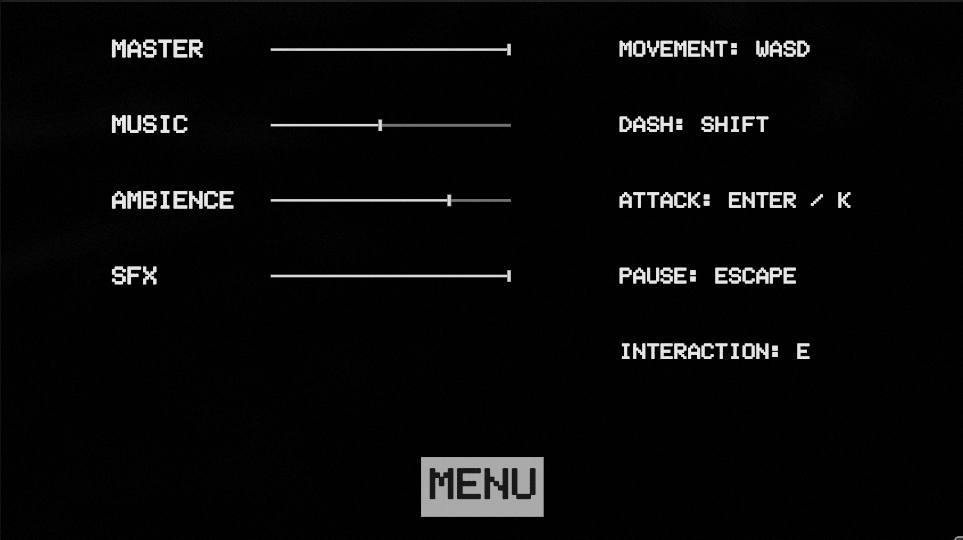
\includegraphics[width=1\textwidth]{img/unity/unity-volume-controls.png}
    \caption{Nastavení hlasitosti}
    \label{fig:unity-volume-controls}
\end{figure}

\begin{figure}[h!]
    \centering
    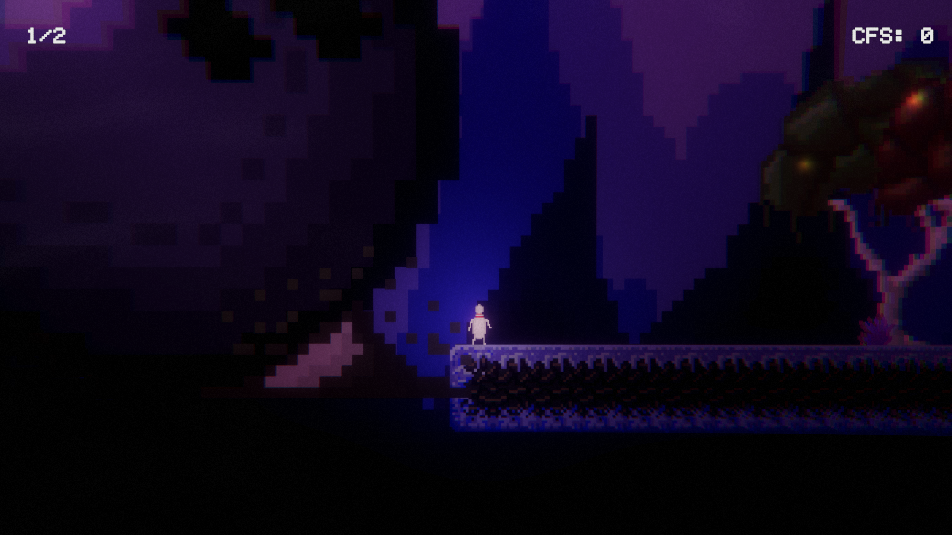
\includegraphics[width=1\textwidth]{img/unity/unity-hud.png}
    \caption{HUD ve hře -- levý horní roh: počet střel, pravý horní roh: počet CFs}
    \label{fig:unity-hud}
\end{figure}

\subsection{Ostatní funkce UI}
\label{sec:ostatni-funkce-ui}

Kromě hlavních panelů a HUD prvků popsaných v předchozí podkapitole existuje v projektu několik dalších vizuálních komponent, které doplňují herní zážitek.

\textbf{Respawn / Checkpoint systém} -- systém checkpointů umožňuje hráči ukládat pozici, na kterou bude respawnován po \emph{soft death} (používáno v \emph{The Exploration}). Checkpoint je objekt ve scéně, s nímž hráč může interagovat stisknutím klávesy \texttt{E}. Při aktivaci se uloží jako referenční bod \newline v komponentě \texttt{DeathZoneSoft}, která po vstupu hráče do svého triggeru okamžitě přesune hráče na pozici posledního aktivovaného \texttt{CheckPoint}u:

\begin{lstlisting}[caption={CheckPoint -- aktivace checkpointu}, label={lst:checkpoint}]
public void Activate()
{
    if (lastActivated != null && lastActivated != this)
        lastActivated.Deactivate();
    lastActivated = this;
    deathZoneSoft.respawnPoint = this.gameObject;
    spriteRenderer.color = Color.green;
}
\end{lstlisting}

V aktuální implementaci se při \emph{soft death} přesouvá pouze pozice hráče -- počet střel i \emph{conversation fragments} zůstávají zachovány. Toto odpovídá designovému rozhodnutí pro \emph{The Exploration}, kde je kladen důraz na průzkum bez trestu. Naproti tomu \emph{The Chase} bude implementovat \emph{hard death}, který skrze reload celé scény obnoví všechny proměnné do výchozího stavu.

\textbf{Camera Respawn Catch} -- komponenta zajišťující plynulé přesunutí kamery k hráči po respawnu. Při volání metody \texttt{OnPlayerRespawn()} se cílová pozice okamžitě nastaví na pozici hráče, takže kamera může pomocí interpolace (\texttt{Vector3.Lerp}) hladce dohnat případný rozestup vzniklý během teleportace.

\textbf{Parallax} -- vizuální komponenta pozadí, která simuluje hloubku prostoru pomocí odlišných rychlostí pohybu jednotlivých vrstev. Sprite renderer na každé vrstvě dostane koeficient \newline \texttt{parallaxEffectX}; nižší hodnota znamená, že vrstva se pohybuje pomaleji než kamera a působí vzdáleněji. Na obrázcích \ref{fig:unity-parallax-close} a \ref{fig:unity-parallax-far} je vidět nastavení bližší vrstvy na 0.45x a vzdálenější vrstvy na 0.7x -- bližší vrstva se pohybuje výrazně pomaleji a působí staticky, zatímco vzdálenější vrstva rychleji následuje kameru, což navozuje dojem prostorové hloubky.

\begin{figure}[h!]
    \centering
    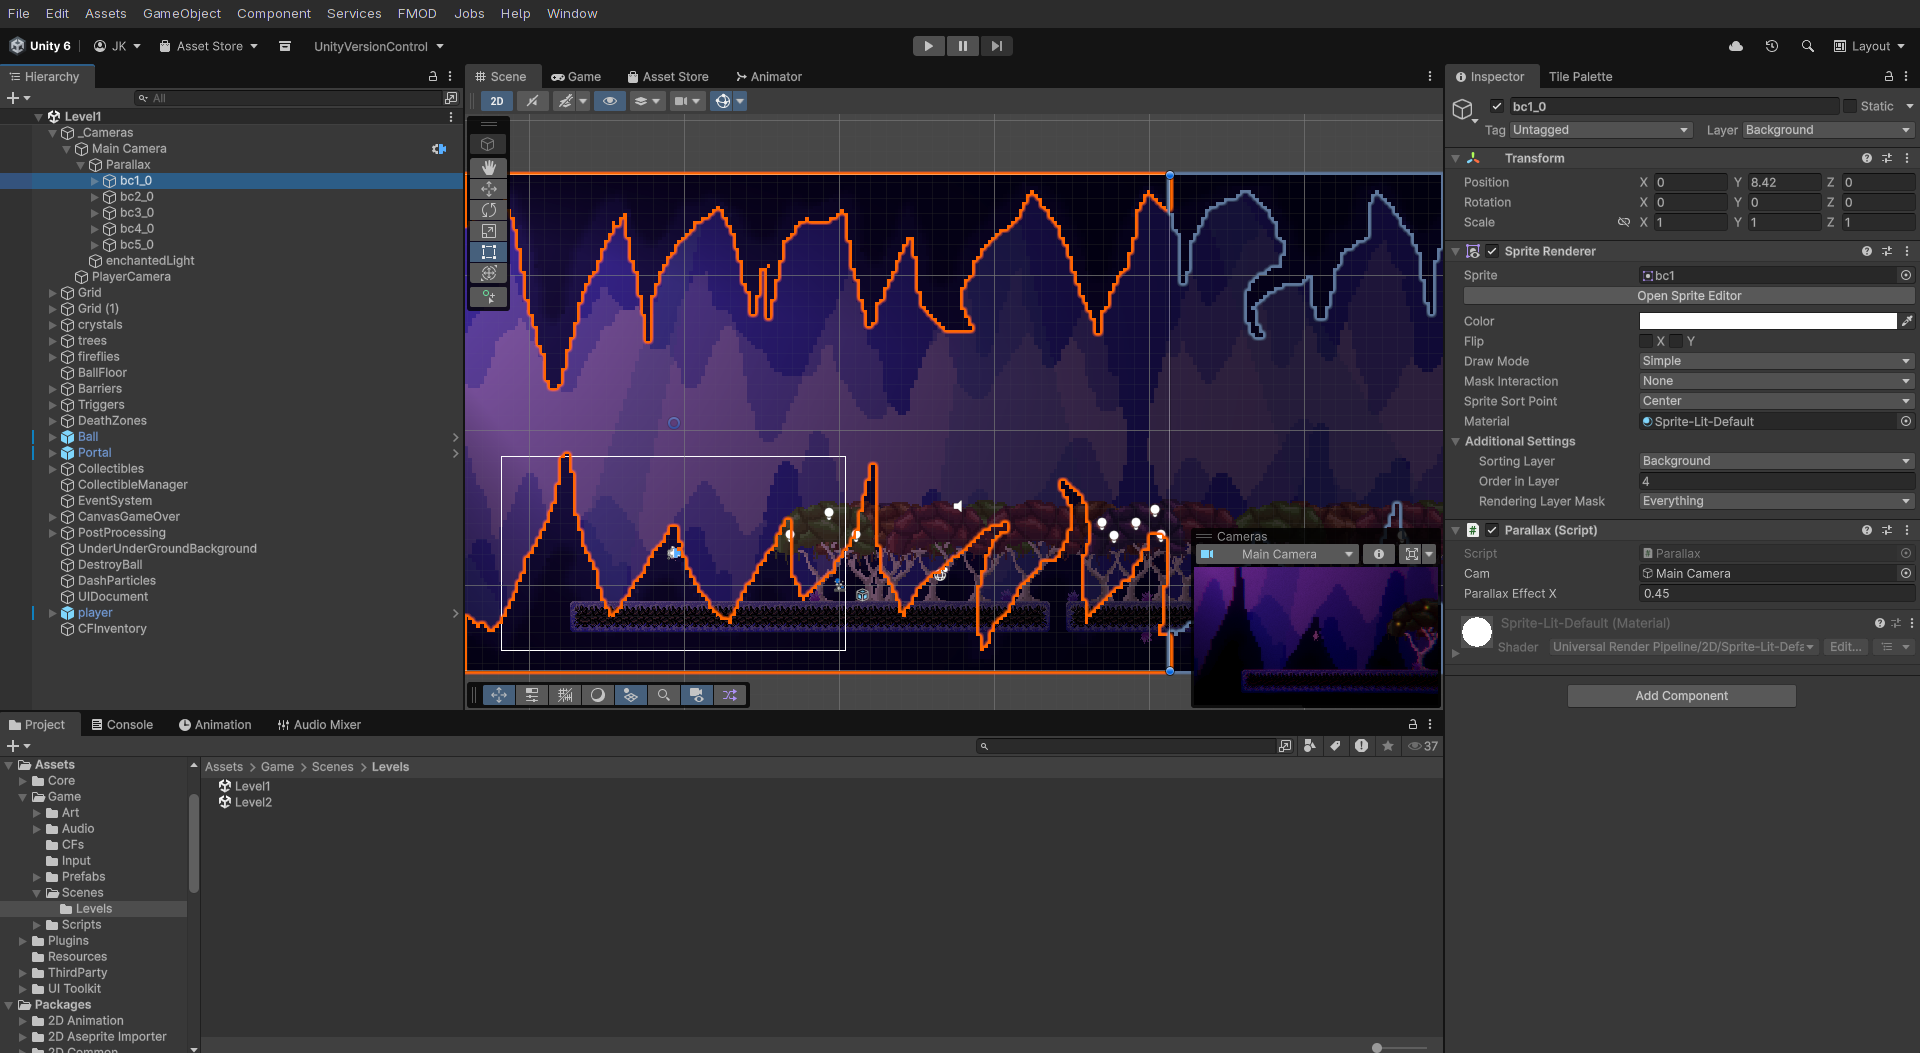
\includegraphics[width=0.8\textwidth]{img/unity/unity-parallax-close.png}
    \caption{Bližší parallax vrstva (\texttt{parallaxEffectX} = 0.45)}
    \label{fig:unity-parallax-close}
\end{figure}

\begin{figure}[h!]
    \centering
    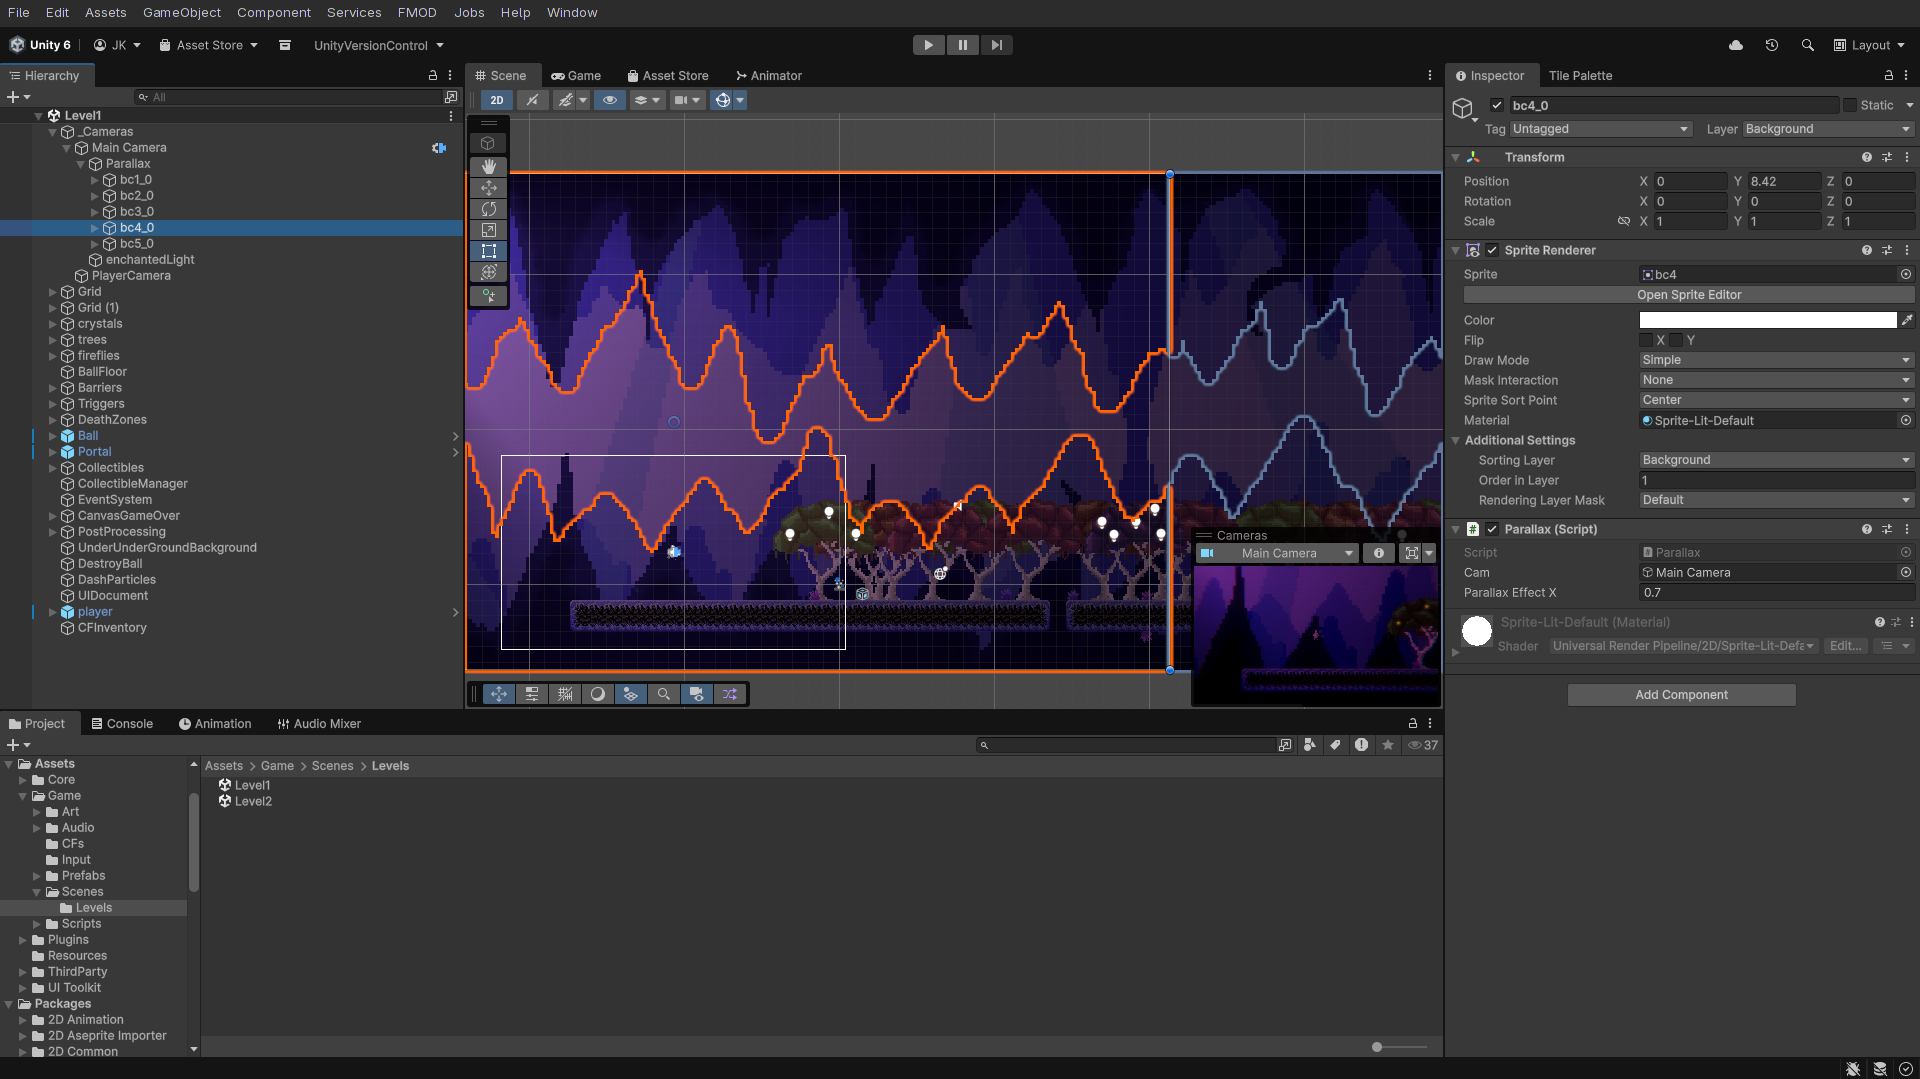
\includegraphics[width=0.8\textwidth]{img/unity/unity-parallax-far.png}
    \caption{Vzdálenější parallax vrstva (\texttt{parallaxEffectX} = 0.7)}
    \label{fig:unity-parallax-far}
\end{figure}

\textbf{Tlačítková hlasová odezva} -- rozšíření \texttt{UIToolkitAudioBinding} přidává k libovolnému \newline \texttt{VisualElement} metodu \texttt{BindHoverSound()}, která registruje callback na událost \texttt{PointerEnterEvent}. Tím se při najetí kurzoru na libovolný element (nejen tlačítka) přehraje zvuk hover efektu, což výrazně zpříjemňuje navigaci v menu a panelech:

\begin{lstlisting}[caption={UIToolkitAudioBinding -- hover zvuk}, label={lst:uitoolkit-hover}]
public static class UIToolkitAudioBinding
{
    public static void BindHoverSound(this VisualElement ve, System.Action play)
    {
        ve.RegisterCallback<PointerEnterEvent>(_ => play());
    }
}
\end{lstlisting}

\section{Tvorba vizuálních efektů}
\label{sec:tvorba-vizualnich-efektu}

\subsection{Light 2D}
\label{sec:light-2d}

Pro osvětlení 2D scény využívám systém \emph{Light 2D}, který je součástí \emph{Universal Render Pipeline}. Na rozdíl od tradičního 3D osvětlení, kde jsou světelné paprsky vysílány ze zdrojů a odrazy osvětlují okolní prostředí, Light 2D funguje invertovaně -- každý objekt ve scéně nese informaci o tom, jak má být osvětlen, a globální světlo tyto vlastnosti zprůměruje a aplikuje. Tento přístup je výrazně méně náročný na výkon a ideální pro stylizované 2D hry.

Jedním z nejdůležitějších prvků osvětlení je \texttt{Light2D} typu \emph{Spot} připojený jako child object k objektu hráče. Toto řešení bylo inspirováno hrou \emph{Ori and the Blind Forest}, kde je postava neustále obklopena jemným světelným polem, které jí umožňuje vidět v temném prostředí. Díky tomu, že je \texttt{GameObject} světla child objectem hráče, automaticky se pohybuje spolu s ním bez nutnosti dalšího kódu.


Kromě individuálních zdrojů světla je ve scéně přítomno také \emph{Global Light 2D}, které nastavuje základní intenzitu a barvu osvětlení pro celou scénu. Tím se zajistí, že objekty bez vlastního zdroje světla nejsou zcela ponořeny do tmy, ale zároveň jsou dostatečně kontrastní, aby vynikla atmosféra temnějších částí levelu.

Dalším typem zdroje světla jsou \emph{světlušky} (\emph{Firefly Lights}) v korunách stromů. Každá instance komponenty \texttt{FireflyLight} řídí intenzitu připojeného \texttt{Light2D} pomocí funkce \texttt{Mathf.PingPong}, která vrací hodnotu v rozsahu 0 až 1 tak, že postupně roste a pak zase klesá, dokola -- výsledkem je hladké rozjasňování a zhasínání světla. Každá instance má navíc náhodný \texttt{randomOffset} (viz ukázka kódu), takže jednotlivé světlušky pulzují nezávisle na sobě a vytvářejí dynamičtější a přirozenější efekt:

\begin{lstlisting}[caption={FireflyLight -- pulzující světlo}, label={lst:firefly-light}]
void Update()
{
    float t = Mathf.PingPong(Time.time * speed + randomOffset, 1f);
    light2D.intensity = Mathf.Lerp(minIntensity, maxIntensity, t);
}
\end{lstlisting}

Collectible objekty (\emph{conversation fragments}) rovněž nesou vlastní \texttt{Light2D} zdroj, který je činí vizuálně nápadnými a usnadňuje hráči jejich vyhledávání v prostředí.

Posledním významným případem využití Light 2D je \texttt{PortalActivator}, který při aktivaci portalu postupně zvyšuje intenzitu jeho světla pomocí \texttt{Mathf.Lerp} v čase -- světlo se rozsvítí v průběhu dvou sekund spolu se sprite průhledností a hlasitostí zvuku:

\begin{lstlisting}[caption={PortalActivator -- fade in portalu}, label={lst:portal-light}]
private IEnumerator FadeInPortalLight()
{
    Light2D portalLight = portalVisual.GetComponentInChildren<Light2D>();
    portalLight.intensity = 0f;

    float elapsed = 0f;
    while (elapsed < fadeDuration)
    {
        elapsed += Time.deltaTime;
        float progress = elapsed / fadeDuration;
        portalLight.intensity = Mathf.Lerp(0f, targetLightIntensity, progress);
        yield return null;
    }
    portalLight.intensity = targetLightIntensity;
}
\end{lstlisting}

\begin{figure}[h!]
    \centering
    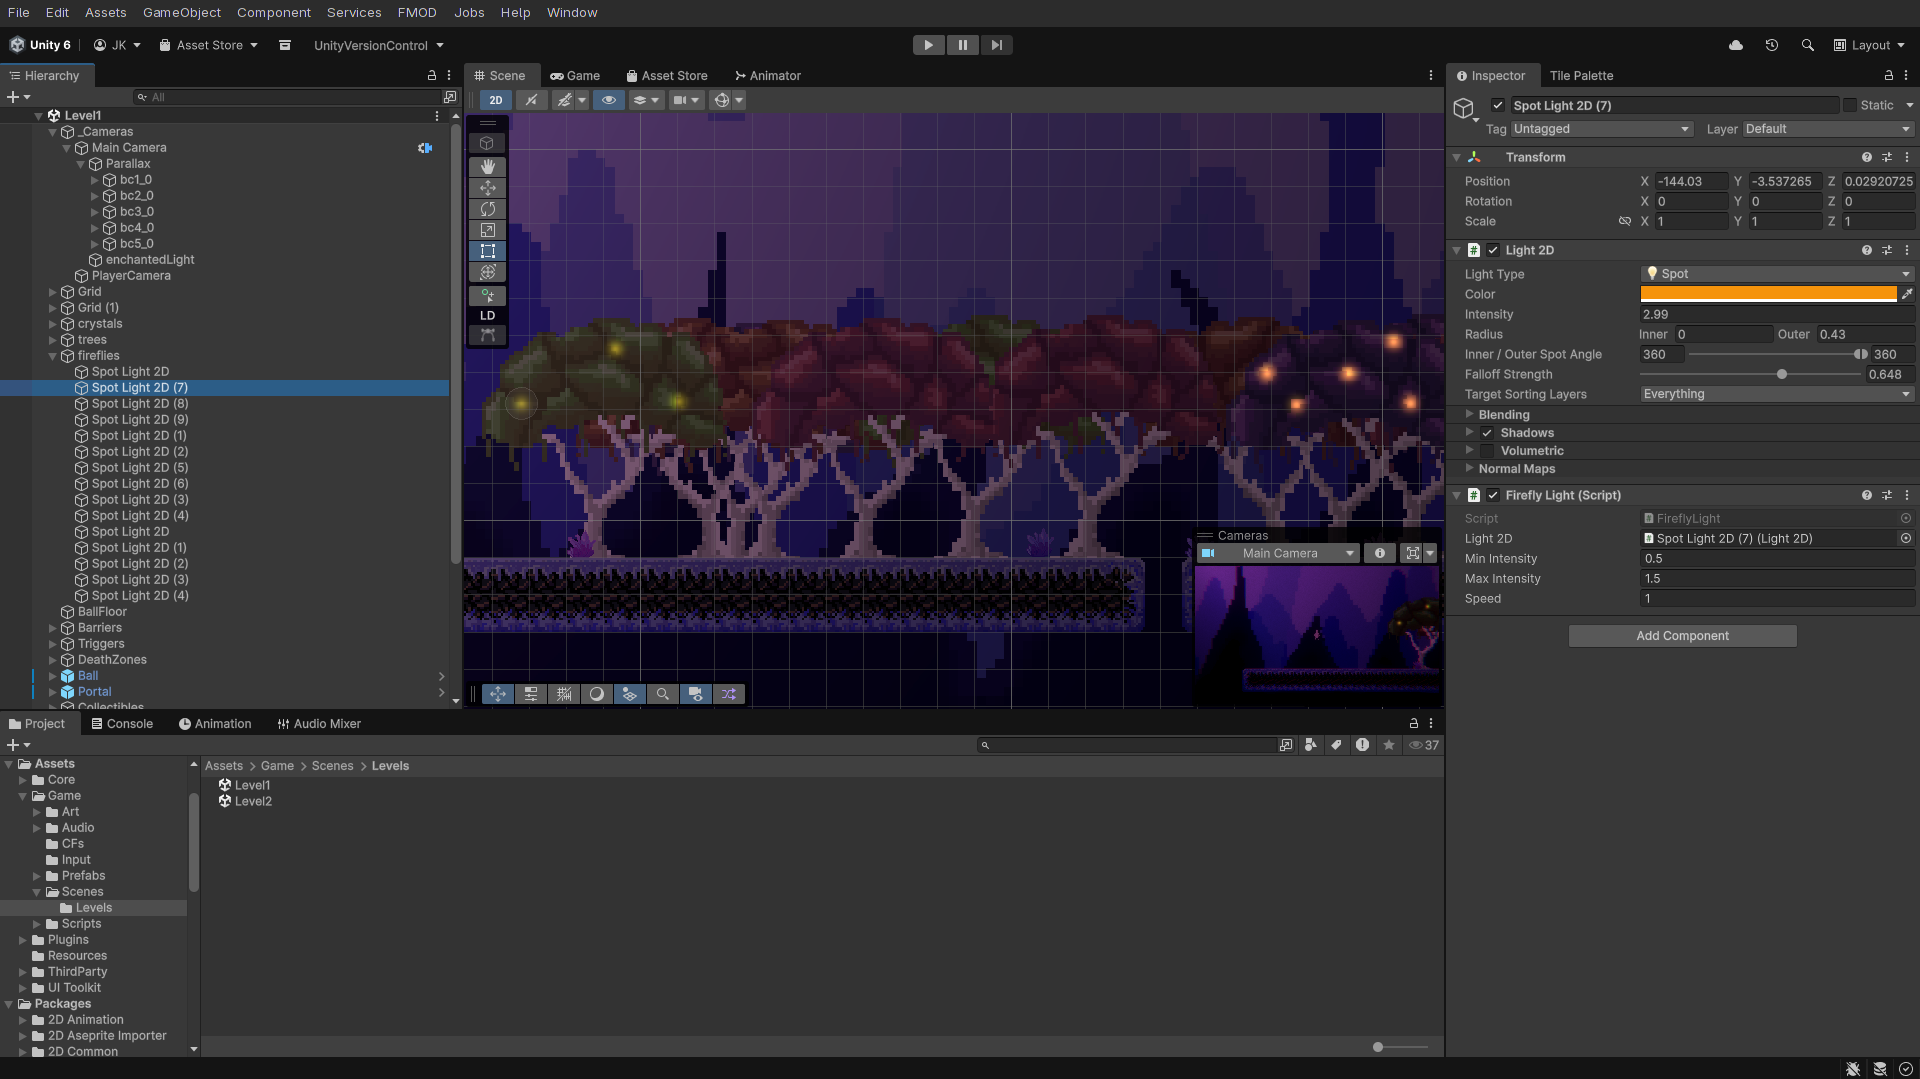
\includegraphics[width=0.8\textwidth]{img/unity/unity-light-firefly.png}
    \caption{Světlušky v korunách stromů ve scéně}
    \label{fig:unity-light-firefly}
\end{figure}

\subsection{Particle System}
\label{sec:particle-system}

Systém částic (Particle System) v Unity umožňuje vytvářet efekt velkého množství malých objektů, které se chovají jako tekutina, kouř, jiskry, nebo v tomto případě -- efekt rychlého úskoku. \newline Při provedení \emph{dash} schopnosti je volána statická metoda \texttt{PlayDashEffect()}, která spustí \newline \texttt{ParticleSystem} na aktuální pozici hráče. Metoda \texttt{Play()} automaticky restartuje animaci částic od začátku, takže není třeba částice před novým spuštěním resetovat. Třída \texttt{DashParticles} využívá singleton vzor, takže může být volána odkudkoliv bez nutnosti držet přímou referenci:

\begin{lstlisting}[caption={DashParticles -- spuštění částic}, label={lst:dash-particles}]
public static void PlayDashEffect(Vector3 position)
{
    if (instance != null)
        instance.TriggerDash(position);
}

private void TriggerDash(Vector3 position)
{
    transform.position = position;
    dashParticles.Play();
}
\end{lstlisting}

Samotný vizuální vzhled částic je definován přímo v Unity editoru v komponentě \newline \texttt{ParticleSystem} -- barva, tvar emitoru, doba životnosti jednotlivých částic a trajektorie jsou nastaveny jako asset a nejsou řízeny kódem.

\subsection{Ostatní efekty}
\label{sec:ostatni-efekty-vfx}

Dalším vizuálním prvkem je komponenta \texttt{OrbBehavior}, která ovlivňuje chování collectible objektů (CFs). Když se hráč nachází v blízkosti collectible, aktivuje se magnetický efekt -- objekt se pomocí \texttt{Vector3.MoveTowards} přibližuje k hráči, dokud ho není možné sebrat. Pokud se hráč od collectible vzdálí, objekt přejde do režimu idle, kdy jemně klesá a stoupá na vertikální ose pomocí funkce \texttt{Mathf.Sin}:

\begin{lstlisting}[caption={OrbBehavior -- magnet a idle animace}, label={lst:orb-behavior}]
float dist = Vector2.Distance(transform.position, player.position);
magnetActive = dist <= magnetRadius;

if (magnetActive)
{
    transform.position = Vector3.MoveTowards(
        transform.position,
        player.position,
        pullSpeed * Time.deltaTime
    );
}
else
{
    float newY = startY + Mathf.Sin(Time.time * frequency) * amplitude;
    transform.position = new Vector3(transform.position.x, newY, transform.position.z);
}
\end{lstlisting}

Další vizuální efekt, který zasahuje do herní mechaniky, je komponenta \texttt{DeathEffect}. \newline Ta ovlivňuje proměnné \texttt{Volume} profilu v rámci \emph{Universal Render Pipeline} -- konkrétně snižuje saturaci obrazu a aplikuje tmavý overlay, čímž vytváří cinematický efekt úmrtí. Jedná se o vizuální efekt, který je však implementován pomocí post-processing nástrojů, a proto je podrobněji rozebrán v kapitole \ref{sec:post-processing-hry}.

\section{Tvorba zvukových efektů}
\label{sec:tvorba-zvukovych-efektu}

\subsection{Audio systém}
\label{sec:audio-system}

Práce se zvukem ve hrách je komplexní téma, které zahrnuje správu mnoha souběžných zvukových stop, jejich prostorové umístění, míchání hlasitostí jednotlivých kanálů a plynulé přechody mezi stavy. V rámci vývoje \emph{Surreal Bowling: Salvation Path} jsem prošel evolucí od čistě Unity AudioMixer řešení k profesionálnímu nástroji FMOD Studio, což přineslo výrazné zlepšení v organizaci, flexibilitě i kvalitě výsledného audia.

%%%%% ---- PŮVODNÍ ŘEŠENÍ ---- %%%%%
\subsubsection{Původní řešení -- Unity AudioMixer}
\label{sec:puvodni-audiomixer}

V původní verzi projektu byl audio systém postaven na Unity vestavěném \texttt{AudioMixeru} \newline a centralizovaném skriptu \texttt{AudioManager.cs}, který využíval singleton vzor. Tento manažer spravoval tři hlavní zvukové kanály -- \emph{Music}, \emph{Diegetic} a \emph{Ambience} -- a byl perzistentní mezi scénami díky metodě \texttt{DontDestroyOnLoad}.

\paragraph{Hierarchie AudioMixeru}
Hierarchie AudioMixeru začíná na kořenovém kanálu \emph{Master}, pod nímž se nacházejí dva hlavní kanály: \emph{Music\_Player} a \emph{SFX\_Player} (viz obrázek \ref{fig:unity-audiomixer}). Kanál \emph{Music\_Player} obsahuje podřízený kanál \emph{Music\_Pause}, který řídí hlasitost hudby při pozastavení hry, a pod ním \emph{Music\_Internal}, kam směřuje samotný \texttt{AudioSource} přehrávající hudbu. Kanál \emph{SFX\_Player} se pak větví na \emph{SFX\_UI} pro uživatelské rozhraní, \emph{SFX\_Pause} pro diegetické zvuky při pauze, \emph{SFX\_Internal} jako centrální kanál pro všechny SFX, a ten se dále dělí na \emph{SFX\_Diegetic\_Ambience} (environmentální ambientní smyčky) a \emph{SFX\_Diegetic\_Player} (zvuky vztahující se k hráči).

\begin{figure}[h!]
    \centering
    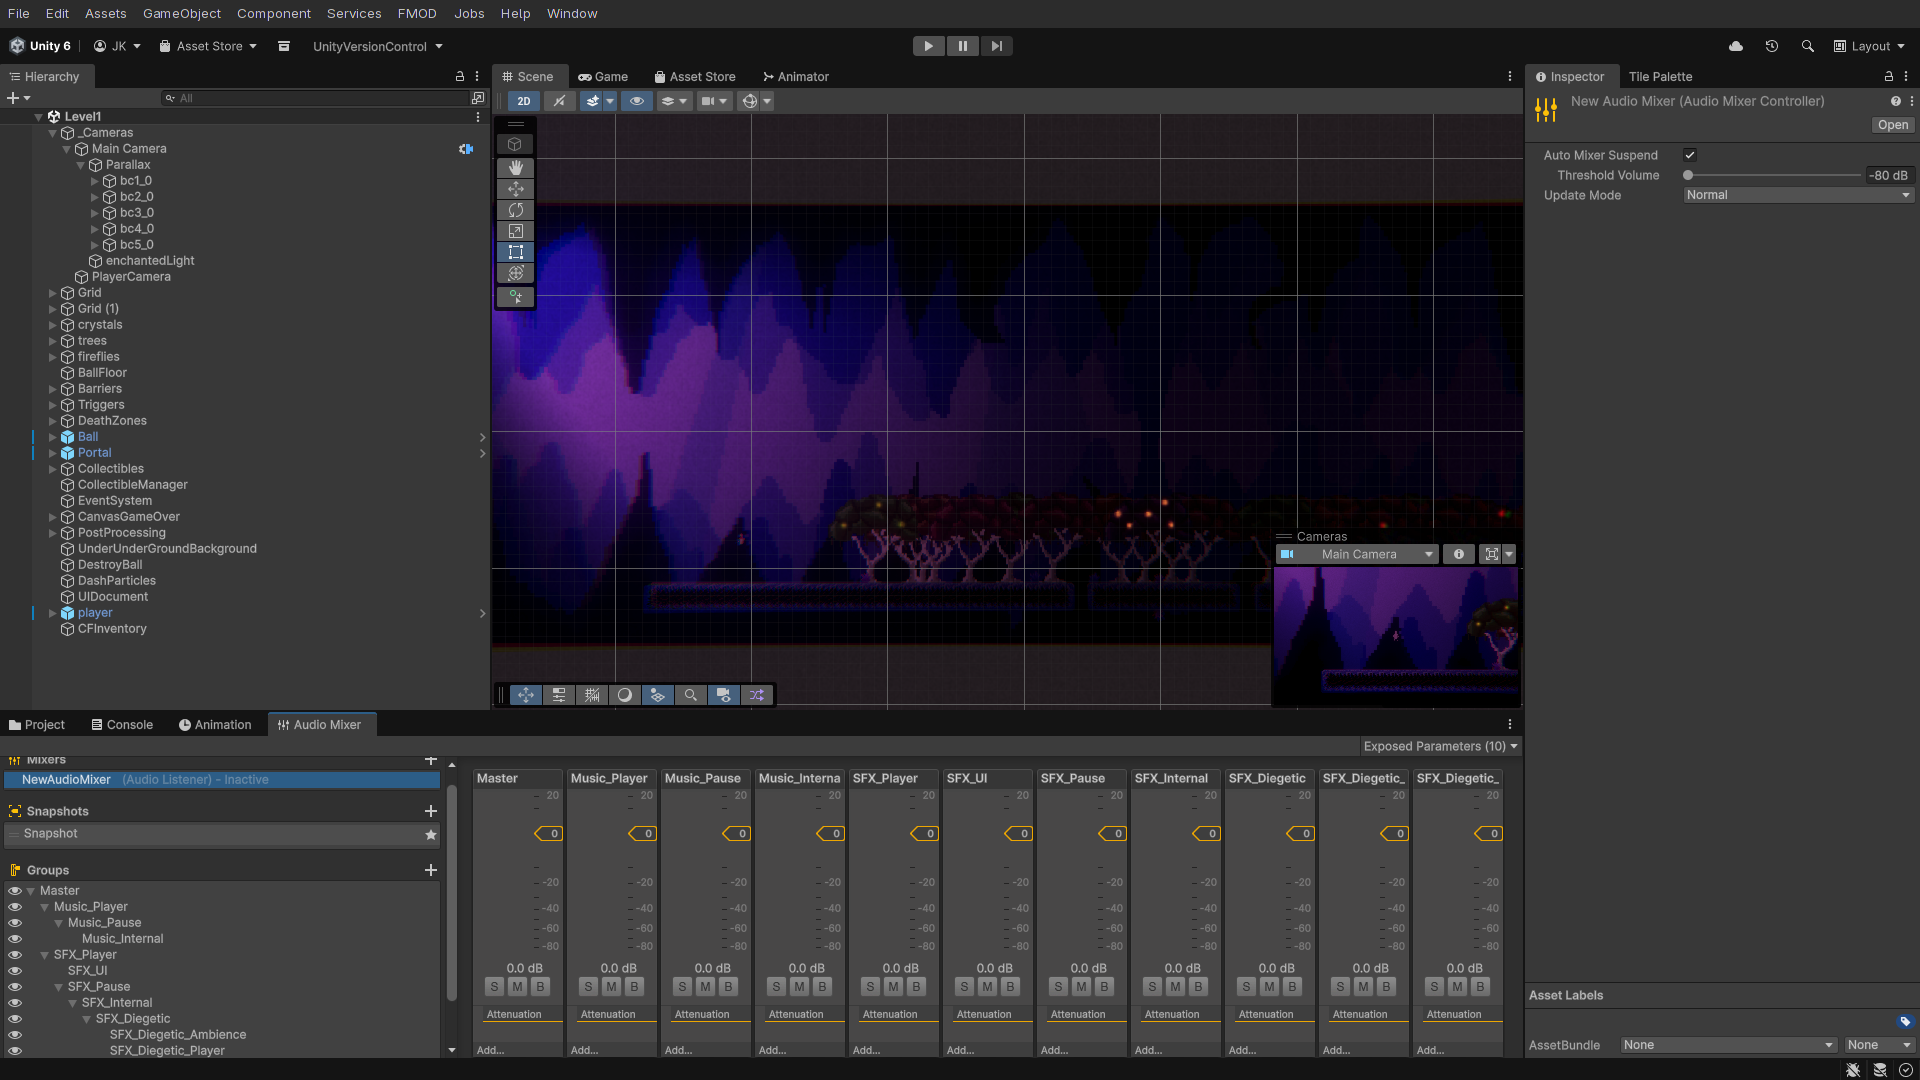
\includegraphics[width=0.9\textwidth]{img/unity/unity-audiomixer.png}
    \caption{Struktura Unity AudioMixeru -- hierarchie kanálů}
    \label{fig:unity-audiomixer}
\end{figure}

\paragraph{Plynulé přechody pomocí \texttt{Lerp}}
Klíčovou funkcí původního systému byla metoda \texttt{FadeAudio()}, která zajišťovala plynulé přechody hlasitosti pomocí lineární interpolace (\texttt{Mathf.Lerp}) mezi aktuální a cílovou hodnotou v decibelech:

\begin{lstlisting}[caption={AudioManager -- plynulý přechod hlasitosti pomocí Lerp}, label={lst:fade-audio-lerp}]
private IEnumerator FadeAudio(string mixerParam, float targetDB, float fadeDuration)
{
    mixer.GetFloat(mixerParam, out float startDB);

    float elapsed = 0f;
    while (elapsed < fadeDuration)
    {
        elapsed += Time.unscaledDeltaTime;
        float t = elapsed / fadeDuration;
        mixer.SetFloat(mixerParam, Mathf.Lerp(startDB, targetDB, t));
        yield return null;
    }
    mixer.SetFloat(mixerParam, targetDB);
}
\end{lstlisting}

Tato korutina byla využívána pro všechny operace vyžadující plynulý přechod -- fade-in a fade-out hudby při přechodu mezi scénami, pozastavení hudby při \texttt{Time.timeScale = 0f}, nebo ztišení diegetických zvuků při úmrtí hráče (\texttt{MuteDiegetic()}). Hodnota \texttt{Time.unscaledDeltaTime} \newline zajišťuje, že fade proběhne v reálném čase i při zastaveném herním čase, což je kritické pro správné fungování při pauze.

Metoda \texttt{PlaySound()} přijímala \texttt{SoundType} enum, pole \texttt{AudioClipů} a přehrávala náhodný klip z pole. Tím se docílilo variace zvuků -- například pro footsteps existovaly tři různé zvukové soubory, z nichž byl pokaždé náhodně vybrán jeden:

\begin{lstlisting}[caption={AudioManager -- přehrání zvuku s náhodnou variací}, label={lst:playsound-oldsystem}]
public static void PlaySound(SoundType sound, AudioSource audioSource, float volume = 1f)
{
    if (instance == null || audioSource == null) return;

    int soundIndex = (int)sound;
    var clips = instance.soundList[soundIndex].Sounds;
    var clip = clips[UnityEngine.Random.Range(0, clips.Length)];
    audioSource.PlayOneShot(clip, volume);
}
\end{lstlisting}

\paragraph{Nevýhody původního přístupu}
Nevýhodou tohoto přístupu byla centralizace veškeré logiky do jednoho skriptu a absence nativní podpory pro pokročilé zvukové techniky jako je crossfading, shuffle (náhodný výběr z více variant s garantovanou unikátností) nebo prostorové zvuky. Proto jsem při přechodu na nejnovější verzi zvolil profesionální nástroj FMOD Studio.

%%%%% ---- FMOD STUDIO ---- %%%%%
\subsubsection{FMOD Studio}
\label{sec:fmod-studio}

FMOD Studio je profesionální zvukový middleware, který umožňuje návrh zvukového obsahu v dedikovaném editoru a následnou integraci do Unity. Pro každou akci ve hře lze vytvořit \emph{Event} -- kontejner, který může obsahovat jeden nebo více zvukových klipů, efekty (EQ, komprese, reverb), mixovací nastavení i parametrické ovladače. Na obrázku \ref{fig:fmod} je zobrazeno prostředí FMOD Studio s otevřeným eventem \texttt{ButtonClick}, který slouží jako ukázka struktury typického eventu -- jsou zde vidět Track s audio clipem, volume envelope a další moduly.

\begin{figure}[h!]
    \centering
    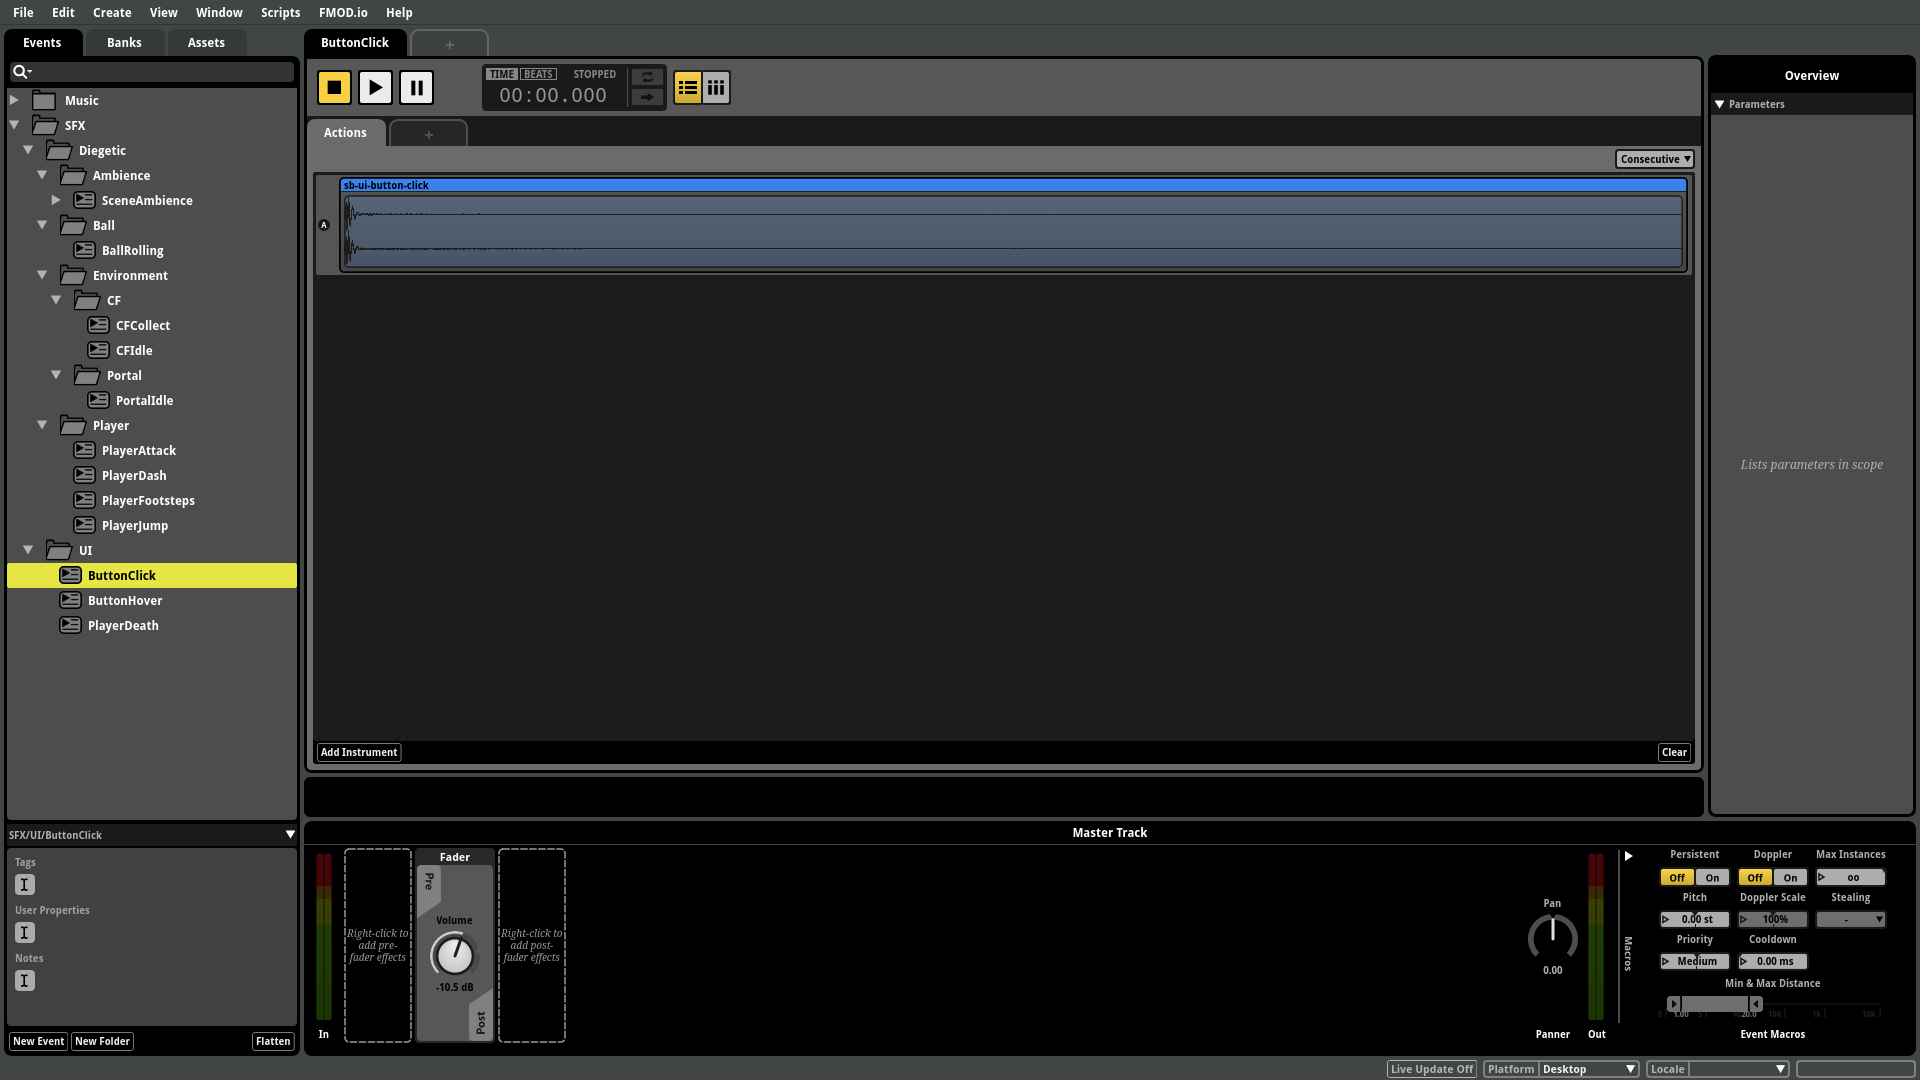
\includegraphics[width=1\textwidth]{img/fmod/fmod.png}
    \caption{FMOD Studio -- prostředí editoru s otevřeným eventem ButtonClick}
    \label{fig:fmod}
\end{figure}

FMOD projekt (\texttt{FMOD\_SB.fspro}) obsahuje tři hlavní \emph{Banky}: \emph{Master}, \emph{Music} a \emph{SFX}. Master bank obsahuje globální nastavení a mixovací cesty (busy), Music bank obsahuje všechny hudební stopy, SFX bank pak veškeré jednotlivé zvukové efekty.

Mixovací struktura v FMOD je podobná struktuře původního Unity AudioMixeru -- existují čtyři hlavní busy: \emph{Master}, \emph{Music}, \emph{Ambience} a \emph{SFX}. Hudba a ambience jsou kontinuální smyčky řízené skriptem, zatímco SFX bus obsahuje všechny jednorázové zvukové efekty.

\paragraph{Architektura FMOD pluginu pro Unity}
Integrace FMOD do Unity je zajištěna oficálním FMOD for Unity pluginem, který přidává do Unity editoru několik komponent a editorových oken. Na obrázku \ref{fig:fmod-unity-wizard} je zobrazeno editační okno FMOD Integration Settings, kde se konfiguruje cesta k FMOD projektu, nastavení bank a parametry runtime inicializace. Základní architektura FMOD v Unity se skládá z několika vrstev:

\begin{figure}[h!]
    \centering
    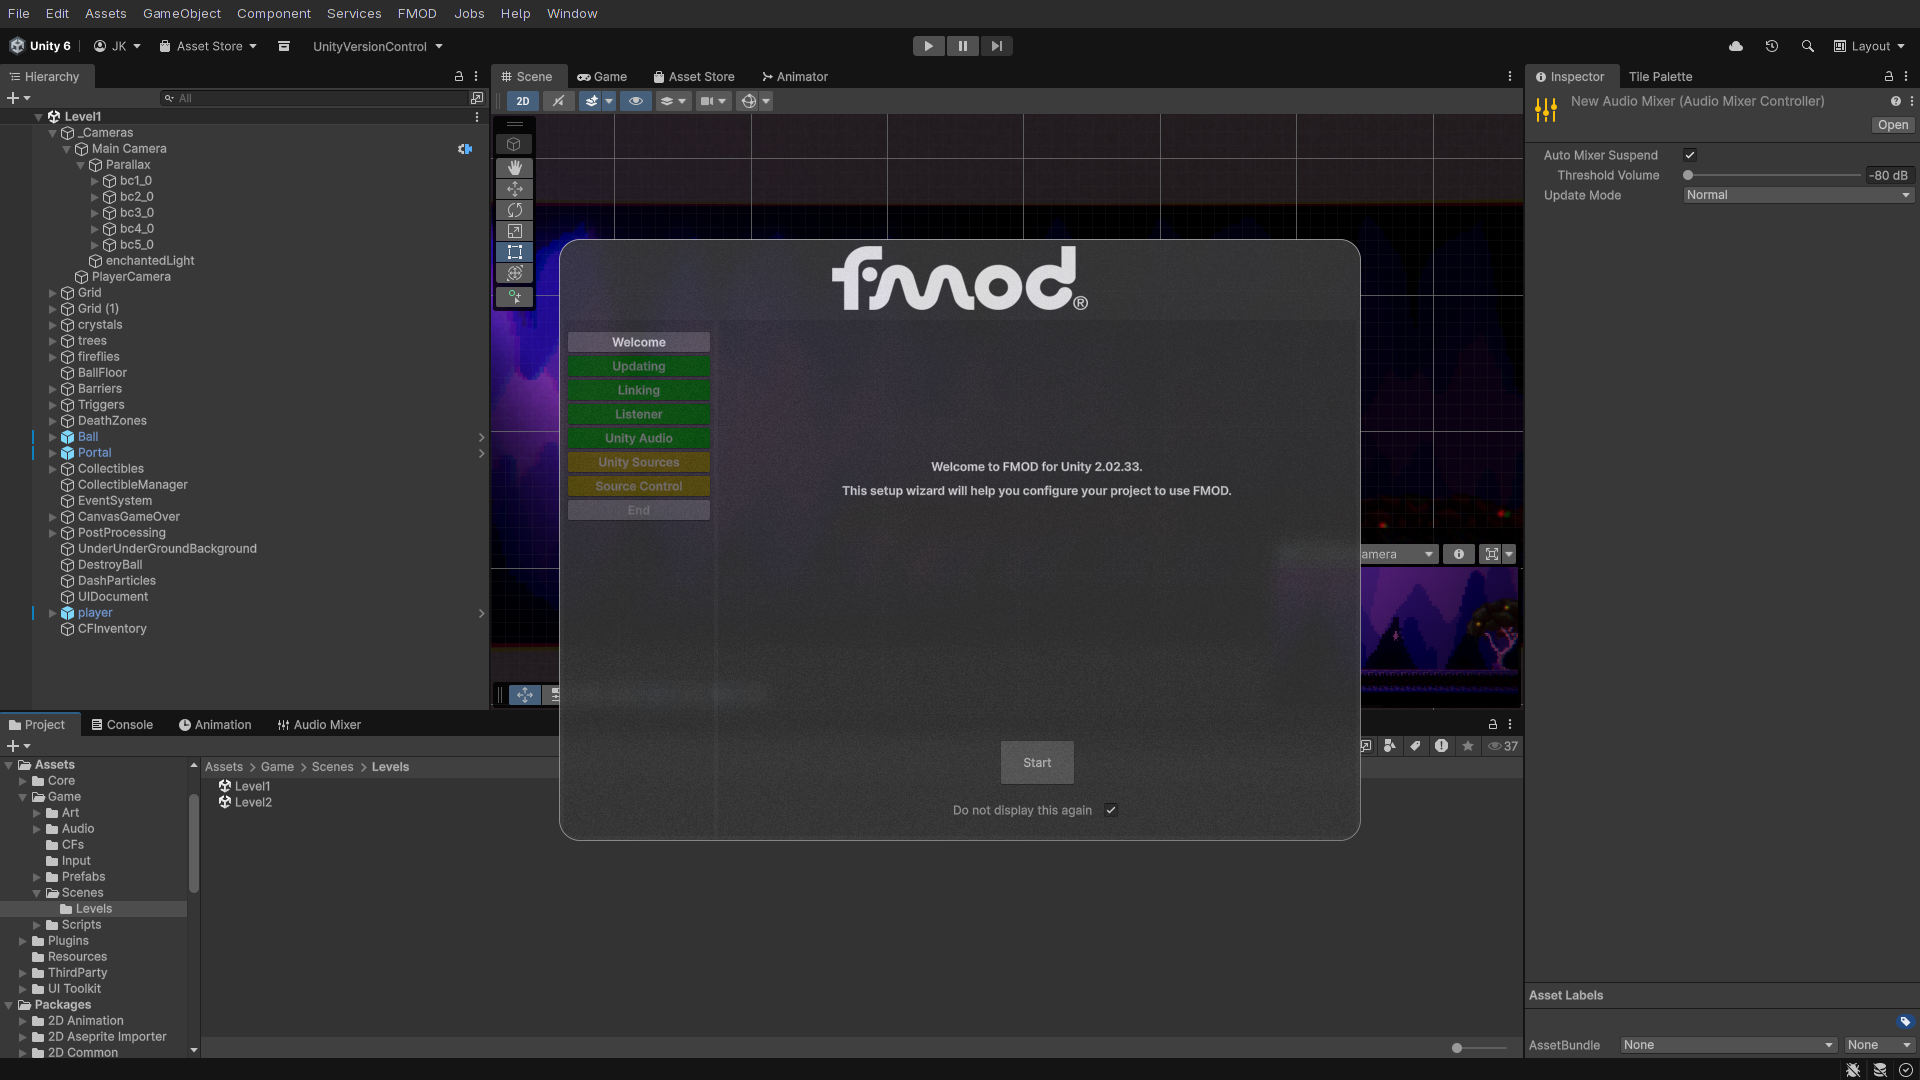
\includegraphics[width=1\textwidth]{img/fmod/fmod-unity-wizard.png}
    \caption{Unity editor -- FMOD Integration Settings}
    \label{fig:fmod-unity-wizard}
\end{figure}

\begin{itemize}
    \item \emph{RuntimeManager} -- inicializuje FMOD runtime při startu aplikace
    \item \emph{StudioEventEmitter} -- komponenta připojená k \texttt{GameObjectu}, která přehrává FMOD eventy na základě herních událostí
    \item \emph{EventReference} -- reference na konkrétní FMOD event, která se binduje v Inspectoru
    \item \emph{EventHandler} -- abstraktní základní třída, která mapuje Unity události (Start, OnDestroy, OnEnable, kolize, triggery) na FMOD akce
\end{itemize}

\paragraph{Komponenta StudioEventEmitter a EmitterGameEvent}
Komponenta \texttt{StudioEventEmitter} je jádrem FMOD integrace v Unity. Její klíčové vlastnosti jsou:

\begin{itemize}
    \item \texttt{EventReference} -- odkaz na FMOD event vytvořený v FMOD Studio
    \item \texttt{EventPlayTrigger} / \texttt{EventStopTrigger} -- určují, jaká Unity událost spustí/zastaví přehrávání
    \item \texttt{AllowFadeout} -- zda má event při zastavení použít fade-out nebo se zastavit okamžitě
    \item \texttt{TriggerOnce} -- zda se event může přehrát pouze jednou
    \item \texttt{Params} -- pole FMOD parametrů, které lze nastavit
\end{itemize}

Enum \texttt{EmitterGameEvent} definuje všechny podporované Unity události, na které lze event navázat:

\begin{itemize}
    \item \texttt{ObjectStart} / \texttt{ObjectDestroy} / \texttt{ObjectEnable} / \texttt{ObjectDisable}
    \item \texttt{TriggerEnter} / \texttt{TriggerExit} a jejich 2D varianty
    \item \texttt{CollisionEnter} / \texttt{CollisionExit} a jejich 2D varianty
    \item \texttt{UIMouseEnter} / \texttt{UIMouseExit} / \texttt{UIMouseDown} / \texttt{UIMouseUp}
\end{itemize}

Základní třída \texttt{EventHandler} (ze které \texttt{StudioEventEmitter} dědí) registruje callbacky na tyto Unity události a při jejich vyvolání volá \texttt{HandleGameEvent()}, která porovnává typ události s nastaveným \texttt{EventPlayTrigger} a \texttt{EventStopTrigger}. Při shodě pak zavolá \texttt{Play()} nebo \texttt{Stop()} na FMOD instanci.

\paragraph{FMODEvents -- centrální registr eventů}
Propojení Unity a FMOD na úrovni kódu zajišťuje singleton \texttt{FMODEvents.cs}, který drží téměř všechny \texttt{EventReference} na jednom místě:

\begin{lstlisting}[caption={FMODEvents -- centrální registr téměř všech FMOD eventů}, label={lst:fmodevents}]
public class FMODEvents : MonoBehaviour
{
    [field: Header("Music")]
    [field: SerializeField] public EventReference music { get; private set; }

    [field: Header("UI")]
    [field: SerializeField] public EventReference buttonClick { get; private set; }
    [field: SerializeField] public EventReference pause { get; private set; }

    [field: Header("Diegetic/Player")]
    [field: SerializeField] public EventReference footsteps { get; private set; }
    [field: SerializeField] public EventReference jump { get; private set; }
    [field: SerializeField] public EventReference dash { get; private set; }

    public static FMODEvents instance { get; private set; }
}
\end{lstlisting}

Jednotlivé FMOD eventy jsou v tomto skriptu definovány jako serializovatelná pole, která lze nastavit v Unity Inspectoru. Tím se odděluje herní logika od konkrétního zvukového obsahu -- změna zvuku nevyžaduje úpravu kódu, pouze přebindování \texttt{EventReference} v editoru.

%%%%% ---- ARCHITEKTURA PŘEHRÁVÁNÍ ---- %%%%%
\subsubsection{Architektura přehrávání zvuků}
\label{sec:architektura-prehravani}

V nejnovější verzi projektu existují dva hlavní, odlišné přístupy k přehrávání zvuků, které odrážejí různou povahu zvukových zdrojů.

\paragraph{PlayOneShot -- jednorázové zvuky}
První přístup využívá \texttt{PlayOneShot()} -- metodu, která vytvoří dočasnou FMOD instanci, přehraje zvuk na zadané pozici a instanci ihned uvolní. Tento model je ideální pro krátké, jednorázové zvuky, u kterých nepotřebujeme sledovat jejich životní cyklus. Příkladem je smrt hráče, \newline kde \texttt{PlayerDeath.cs} volá:

\begin{lstlisting}[caption={PlayOneShot -- jednorázový zvuk}, label={lst:playoneshot}]
AudioManager.instance.PlayOneShot(FMODEvents.instance.death, this.transform.position);
\end{lstlisting}

\paragraph{StudioEventEmitter -- looping objekty}
Druhý přístup využívá \texttt{StudioEventEmitter} komponentu připojenou přímo k \texttt{GameObjectu}. Tento model je vhodný pro zvuky, které jsou vázány na životní cyklus objektu nebo na jeho herní stav. Pro \emph{looping} objekty, jako je valicí se \emph{Ball}, je na tomto \texttt{GameObjectu} v prefabu připojena komponenta \texttt{StudioEventEmitter} s nastavením \texttt{EventPlayTrigger = ObjectStart} a \texttt{EventStopTrigger = ObjectDestroy}. FMOD event se tak spustí při vytvoření objektu a hraje v nekonečné smyčce, dokud objekt není zničen (např. při dopadu do destrukční zóny), pak se event ukončí s fade-outem.

\paragraph{One-shot objekty s vlastním emitorem}
Pro \emph{one-shot objekty}, které mají svůj vlastní event emitor, existují dva přístupy. Prvním je vázání na \texttt{ObjectDestroy} -- když je \texttt{GameObject} zničen (například při sebrání collectible), FMOD event se přehraje. Typickým příkladem je \texttt{Collectible} (CF -- Conversation Fragment), kde druhý \newline \texttt{StudioEventEmitter} na objektu přehrává zvuk sebrání:

\begin{lstlisting}[caption={Collectible prefab -- dva FMOD emitory}, label={lst:collectible-emitters}]
// Emitter 1 -- idle/ambient zvuk
StudioEventEmitter:
  EventReference: event:/SFX/Diegetic/Environment/CF/CFIdle
  EventPlayTrigger: ObjectStart
  EventStopTrigger: ObjectDestroy

// Emitter 2 -- zvuk při sebrání
StudioEventEmitter:
  EventReference: event:/SFX/Diegetic/Environment/CF/CFCollect
  EventPlayTrigger: ObjectDestroy
  EventStopTrigger: None
\end{lstlisting}

Na objektu CF jsou tedy dva \texttt{StudioEventEmitter} komponenty -- první se spustí při vytvoření objektu a vydává ambientní zvuk, druhý se spustí až při zničení objektu (sebrání hráčem). V Inspectoru Unity jsou tyto dvě komponenty zobrazeny v dolní části, jak ukazuje obrázek \ref{fig:fmod-unity-emitter}.

\begin{figure}[h!]
    \centering
    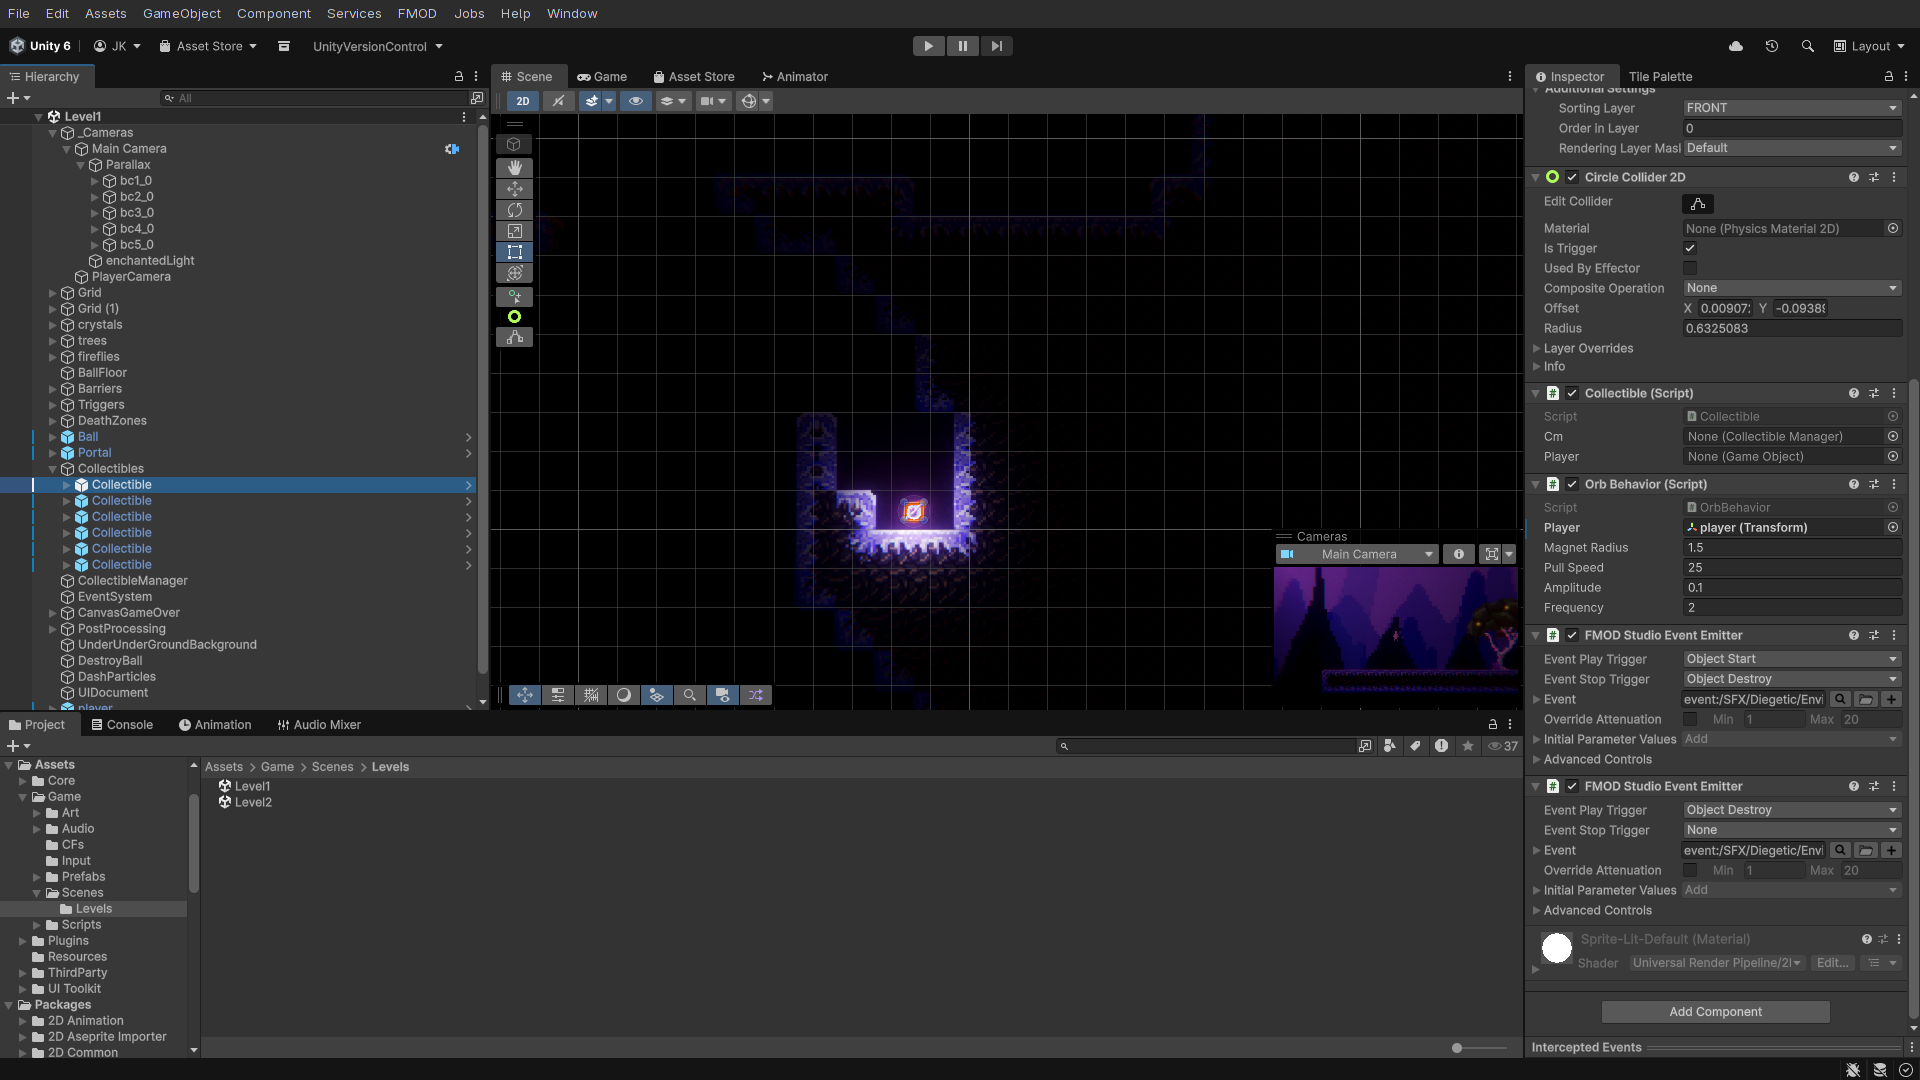
\includegraphics[width=1\textwidth]{img/fmod/fmod-unity-emitter.png}
    \caption{Dvě komponenty \texttt{StudioEventEmitter} připojené k objektu CF}
    \label{fig:fmod-unity-emitter}
\end{figure}

Druhý přístup pro one-shot objekty spočívá ve využití \texttt{RuntimeManager.PlayOneShot()} přímo v kódu, což je vhodné pro situace, kdy chceme mít plnou kontrolu nad timingem přehrávání.

%%%%% ---- VAZBA ZVUKŮ NA ANIMACE ---- %%%%%
\subsubsection{Vazba zvuků na animace}
\label{sec:vazba-zvuku-na-animace}

Zvuky je možné navázat přímo na animace pomocí Unity \emph{Animation Events}. Tato technika umožňuje, aby v konkrétním snímku animace byla zavolána libovolná metoda na libovolném skriptu připojeném k \texttt{GameObjectu}. Příkladem jsou kroky hráče -- animace \texttt{player\_run.anim} obsahuje dva Animation Events:

\begin{lstlisting}[caption={Animation Event v player\_run.anim -- PlayFootsteps}, label={lst:anim-event-footsteps}]
m_Events:
  - time: 0.1
    functionName: PlayFootsteps
    objectReferenceParameter: {fileID: 0}
  - time: 0.33333334
    functionName: PlayFootsteps
    objectReferenceParameter: {fileID: 0}
\end{lstlisting}

Na obrázku \ref{fig:fmod-unity-animation-event} je vidět, jak tyto Animation Events vypadají přímo v Unity Editoru -- na časové ose animace jsou zobrazeny značky událostí volající specifické metody.

\begin{figure}[h!]
    \centering
    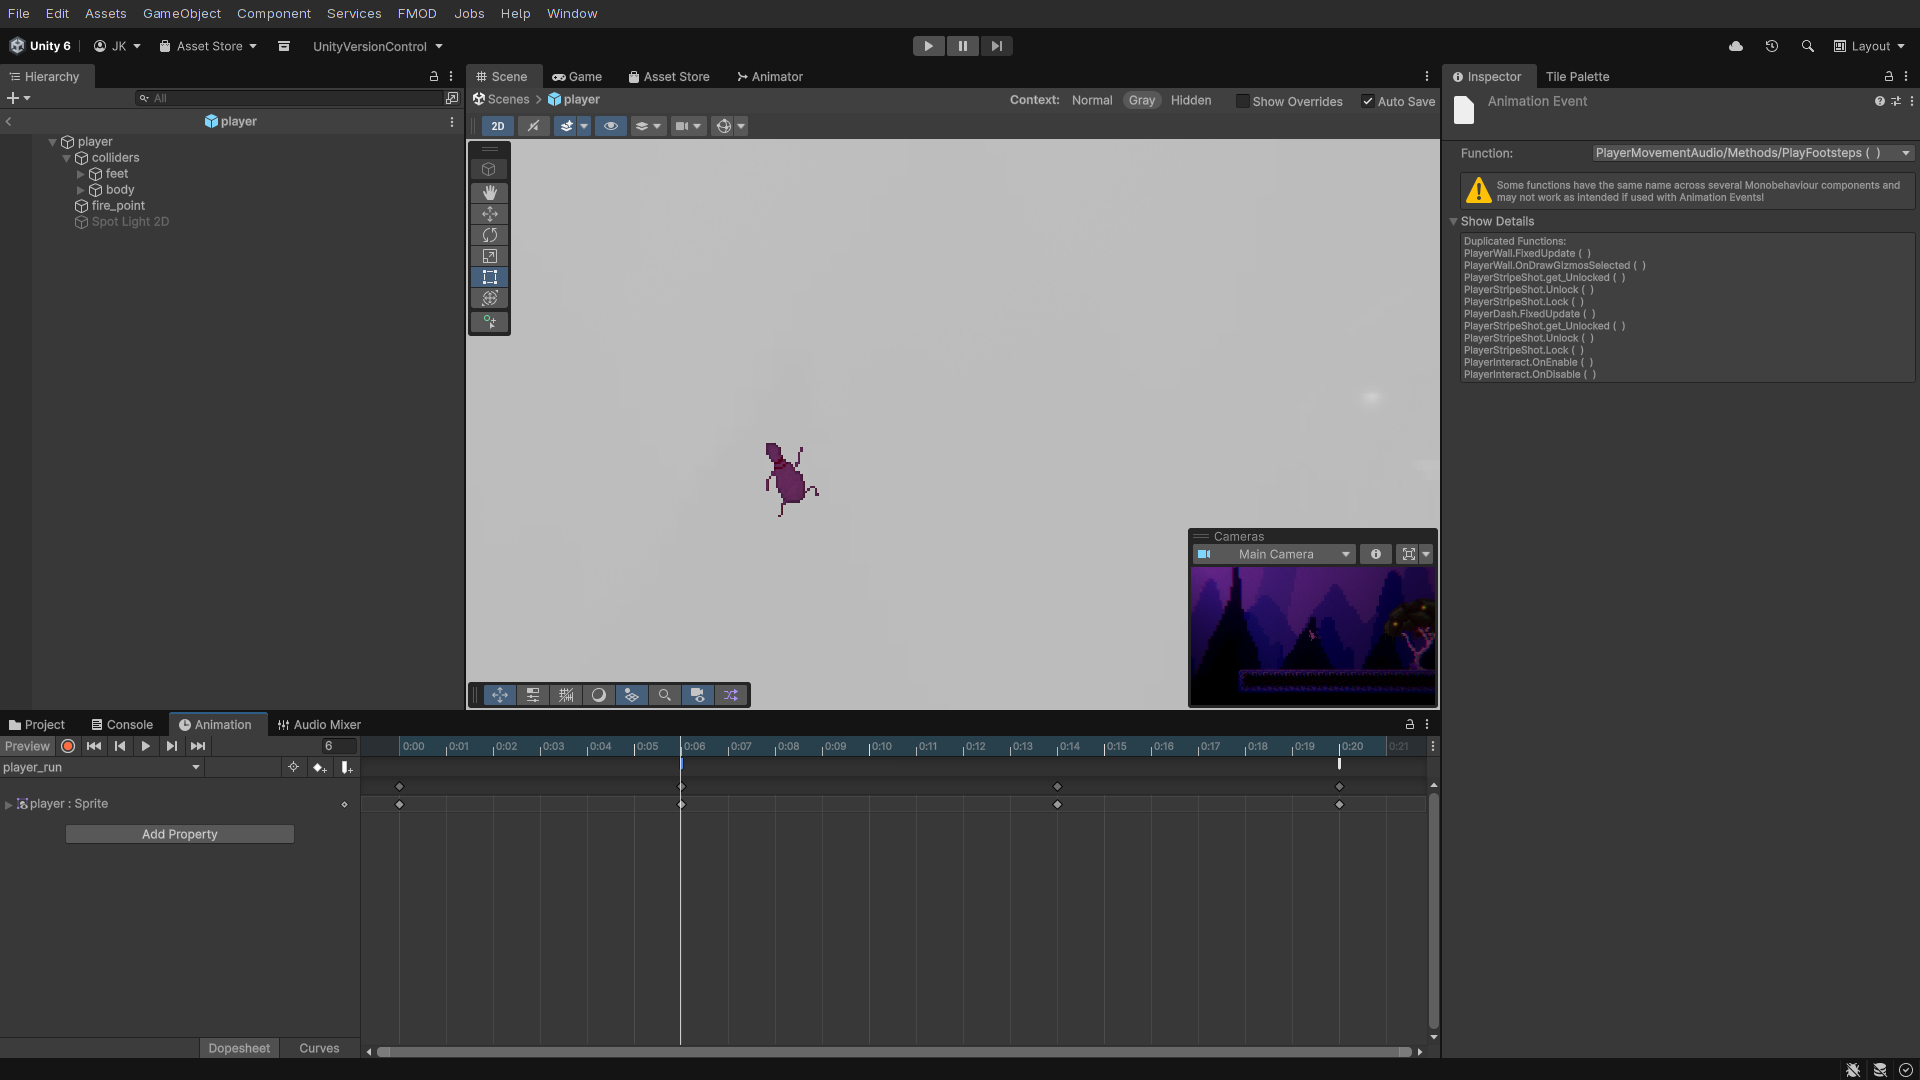
\includegraphics[width=1\textwidth]{img/fmod/fmod-unity-animation-event.png}
    \caption{Animation Events v Unity Editoru}
    \label{fig:fmod-unity-animation-event}
\end{figure}

Tyto events volají metodu \texttt{PlayFootsteps()} na skriptu \texttt{PlayerMovementAudio.cs}, který je připojen k objektu hráče:

\begin{lstlisting}[caption={PlayerMovementAudio -- obsluha footsteps a jump}, label={lst:playermovementaudio}]
public class PlayerMovementAudio : MonoBehaviour
{
    public void PlayFootsteps()
    {
        AudioManager.instance.PlayOneShot(FMODEvents.instance.footsteps, transform.position);
    }

    public void PlayJump()
    {
        AudioManager.instance.PlayOneShot(FMODEvents.instance.jump, transform.position);
    }
}
\end{lstlisting}

Metoda \texttt{PlayFootsteps()} je volána ve dvou snímcích běžící animace (na 0.1 s a 0.333 s), což odpovídá přirozenému rytmu běhu. Podobně animace \texttt{player\_jump.anim} obsahuje Animation Event na snímku 0s, který volá \texttt{PlayJump()}. Výhodou tohoto přístupu je dokonalá synchronizace zvuku s animací bez nutnosti sledovat stav animace v kódu.

Na straně FMOD je footsteps event řešen jako \emph{multiinstrument} -- kontejner, který vybírá z více zvukových stop. Na obrázku \ref{fig:fmod-footsteps} je vidět nastavení shuffle módu, který zajišťuje, že při každém výběru stopy je vybrána vždy jiná varianta, dokud nejsou všechny vyčerpány. Teprve poté se cyklus opakuje -- tím je zaručena určitá míra náhoditosti, ale zároveň zajištěno, že dva po sobě jdoucí kroky nikdy nezní stejně.

\begin{figure}[h!]
    \centering
    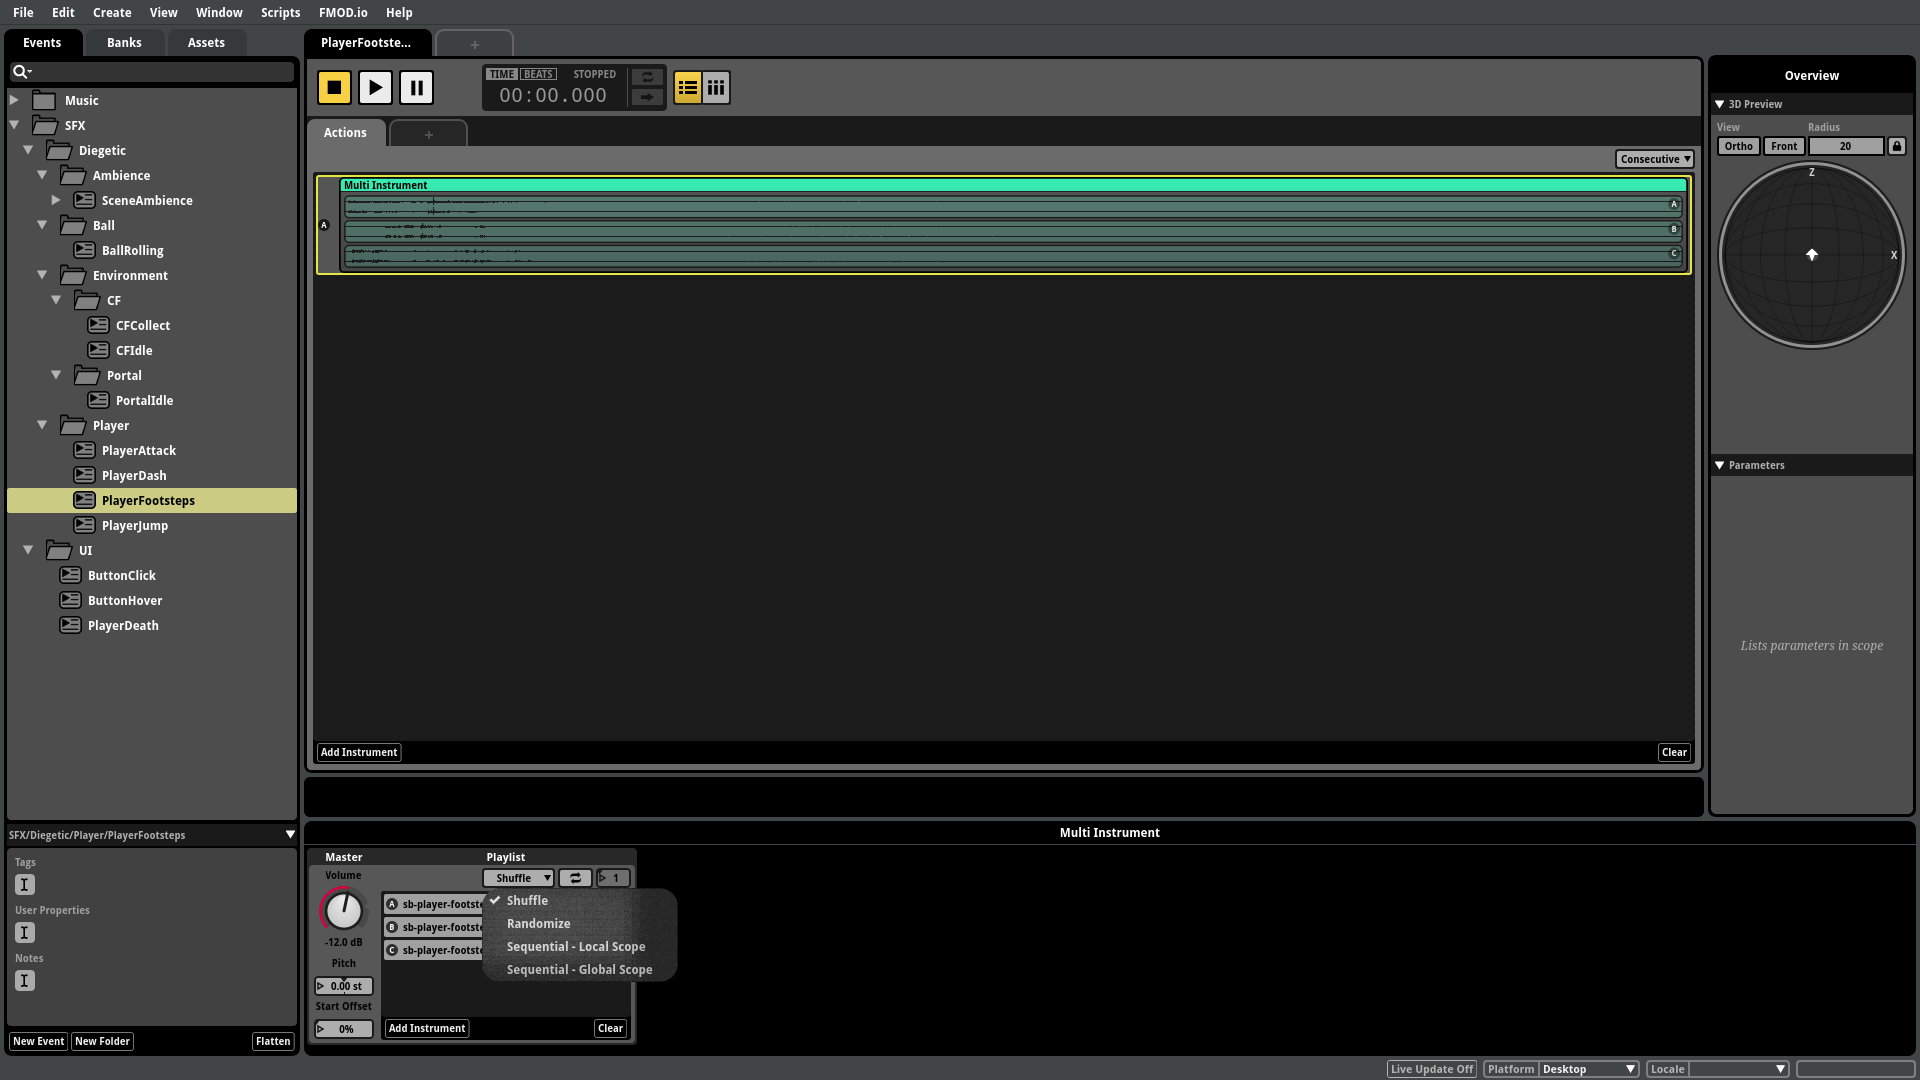
\includegraphics[width=0.9\textwidth]{img/fmod/fmod-footsteps.png}
    \caption{FMOD Studio -- multiinstrument footsteps s aktivním shuffle módem}
    \label{fig:fmod-footsteps}
\end{figure}

%%%%% ---- MUSIC A AMBIENCE ---- %%%%%
\subsubsection{Hudba a Ambience}
\label{sec:hudba-a-ambience}

Hudba a ambience jsou v FMOD řešeny jako kontinuální eventy, které se nespouštějí přes \newline \texttt{PlayOneShot()}, ale přes správu \emph{EventInstance}. Nový \texttt{AudioManager.cs} vytváří při startu dvě dlouhožijící instance -- jednu pro hudbu a jednu pro ambience:

\begin{lstlisting}[caption={AudioManager -- správa hudby a ambience pomocí EventInstance}, label={lst:audio-manager-music}]
public class AudioManager : MonoBehaviour
{
    private EventInstance musicEventInstance;
    private EventInstance ambienceEventInstance;
    private List<EventInstance> eventInstances;

    private void Start()
    {
        InitializeAmbience(FMODEvents.instance.ambience);
        InitializeMusic(FMODEvents.instance.music);
    }

    private void InitializeMusic(EventReference musicEventReference)
    {
        musicEventInstance = CreateEventInstance(musicEventReference);
        musicEventInstance.start();
    }
}
\end{lstlisting}

Pro přepínání hudby a ambience mezi scénami využívám systémy \texttt{MusicChangeTrigger} a \newline \texttt{AmbienceChangeTrigger}, které reagují na událost \texttt{SceneManager.sceneLoaded}. Každá scéna má definovanou odpovídající hodnotu parametru:

\begin{lstlisting}[caption={SceneMusic enum -- mapování scén na FMOD parametry}, label={lst:scenemusic-enum}]
public enum SceneMusic
{
    MAIN_MENU = 0,
    LEVEL_1 = 3,
    LEVEL_2 = 7
}
\end{lstlisting}

V FMOD Studiu je na hudebním eventu vytvořen diskrétní \texttt{Parameter} s názvem \texttt{SceneMusic}. Hudební event obsahuje pro každou hodnotu parametru navázanou jinou hudební stopu -- při změně parametru na hodnotu 3 se crossfadem začne přehrávat hudba pro Level 1, při změně na 0 hudba pro MainMenu. Unity skript pak volá:

\begin{lstlisting}[caption={MusicChangeTrigger -- změna hudby při načtení scény}, label={lst:musicchangetrigger}]
public void SetSceneMusic(SceneMusic scene)
{
    if (!musicEventInstance.isValid()) return;

    float targetValue = (float)scene;
    musicEventInstance.setParameterByName("SceneMusic", targetValue);
}
\end{lstlisting}

Systém \texttt{AmbienceChangeTrigger} funguje identicky, pouze s enumem \texttt{SceneAmbience} a FMOD parametrem \texttt{SceneAmbience}. Toto řešení má výhodu v tom, že oba zvukové systémy jsou perzistentní mezi scénami a přechody jsou plynulé, protože crossfading řeší FMOD interně na základě nastavení parametru. Technicky je efekt plynulého přechodu realizován pomocí automatizace hlasitosti -- v FMOD Studiu je v \emph{Parameter Sheet} každé hudební stopy nastaven AHDSR (Attack-Hold-Decay-Sustain-Release) envelope, konkrétně modul \emph{Volume} s automatizační křivkou, která definuje hlasitostní křivku pro každou hodnotu parametru \texttt{SceneMusic} nebo \texttt{SceneAmbience}. Když skript změní hodnotu parametru, FMOD interpoluje mezi těmito automatizačními body a výsledkem je hladký crossfade mezi jednotlivými stopami bez nutnosti jakéhokoliv kódu navíc.

\begin{figure}[h!]
    \centering
    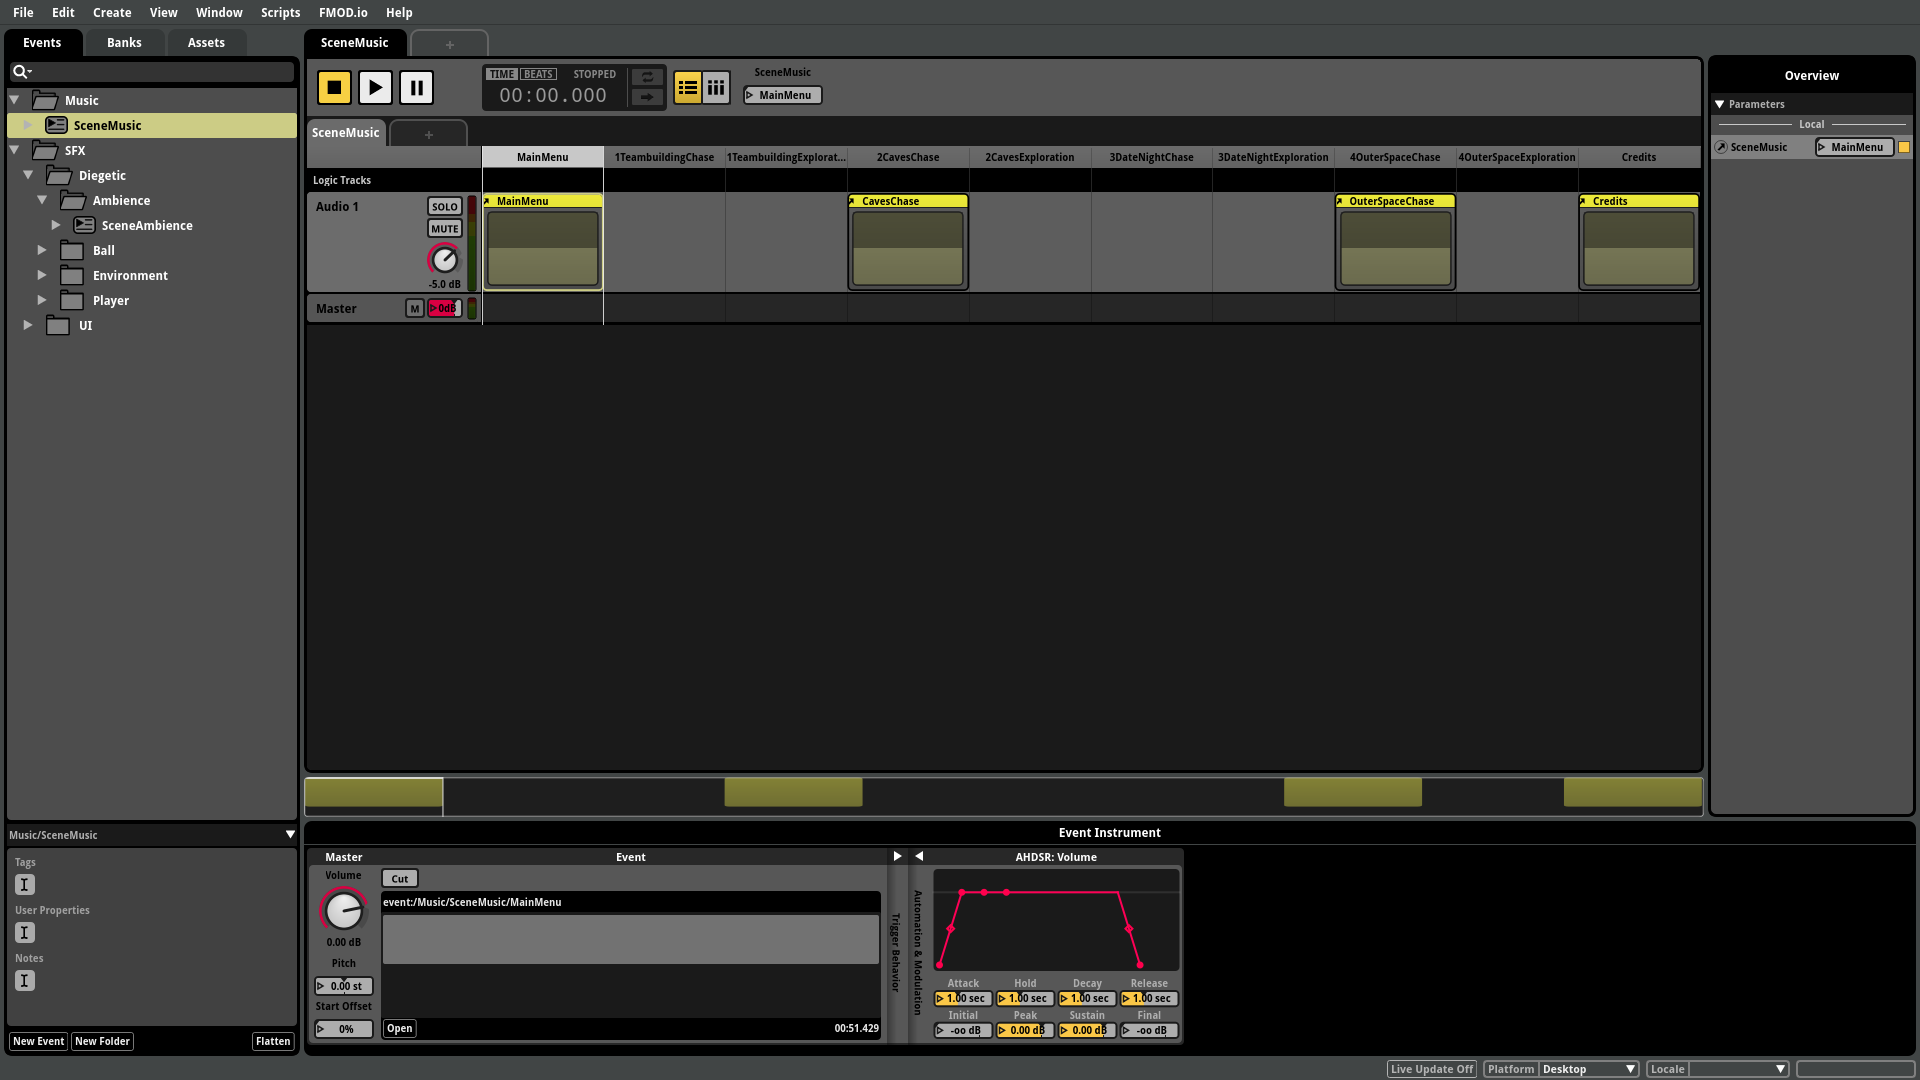
\includegraphics[width=1\textwidth]{img/fmod/fmod-parameter-sheet.png}
    \caption{Parameter Sheet v FMOD Studiu}
    \label{fig:fmod-parameter-sheet}
\end{figure}


\subsection{Tvorba v FL Studio}
\label{sec:tvorba-v-fl-studio}

Práce v FL Studio je jádrem mé audio workflow. Struktura projektu je navržena tak, aby podporovala jak jednotlivé skladby, tak jejich vzájemnou konzistenci v rámci budoucího alba.

\subsubsection{Workflow pomocí Arrangements}
Jedním z hlavních prvků mojí workflow je systém \emph{Arrangements} (Arrangement view). V jediném projektu vytvářím více arrangements, z nichž každý reprezentuje jednu skladbu nebo skupinu \newline zvukových efektů. Důležité je, že všechny arrangements sdílejí stejnou sadu pluginových presetů a jsou napojeny na shodné Mixer kanály. Tím je zajištěno, že nástroje a zvuky použité napříč různými skladbami zní jednotně -- stejný syntezátor v odlišném arrangements posílá signál do stejného Mixer kanálu, což vytváří koherentní zvukový profil celého alba. Tento přístup eliminuje problém rozdílně nastavených kanálů mezi skladbami a značně zjednodušuje finální mix.

\begin{figure}[h!]
    \centering
    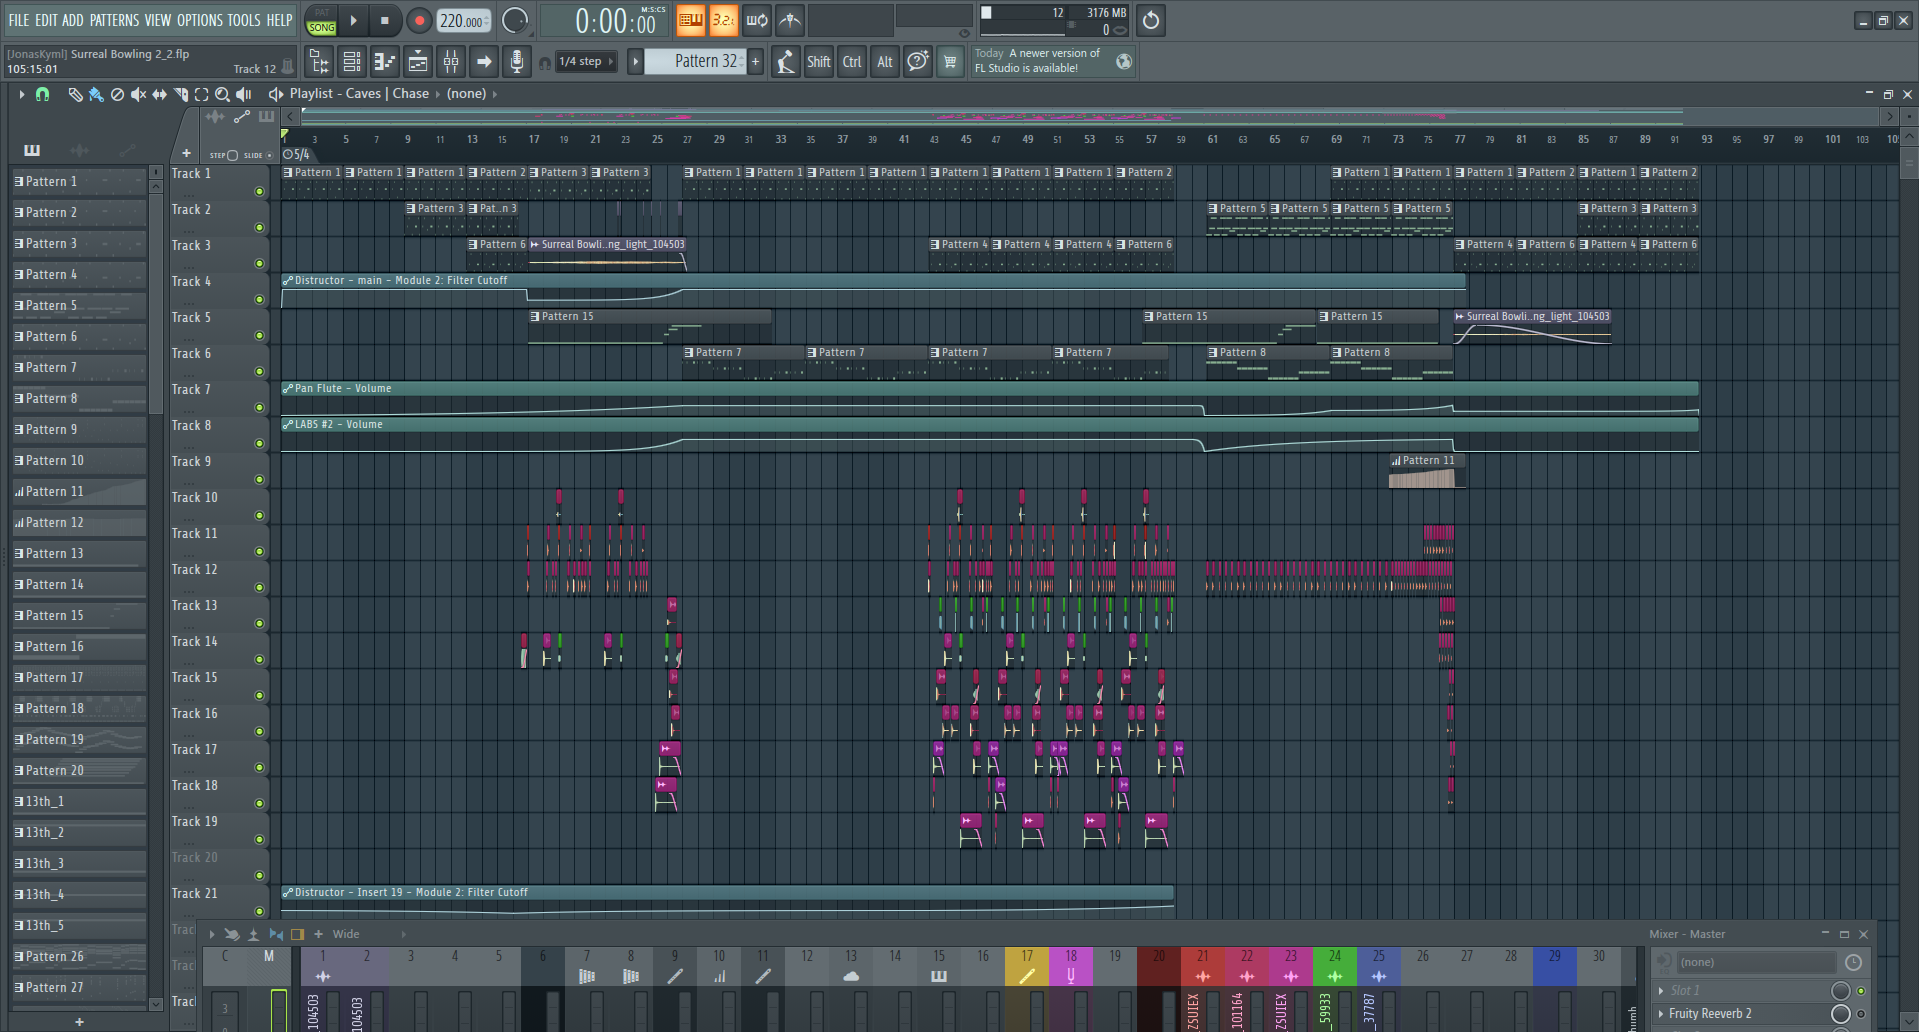
\includegraphics[width=1\textwidth]{img/flstudio/flstudio-arrangement.png}
    \caption{FL Studio -- Arrangement view}
    \label{fig:flstudio-arrangement}
\end{figure}

Jak je vidět na obrázku \ref{fig:flstudio-arrangement}, každý arrangement obsahuje více stop (tracks), přičemž každá stopa může obsahovat jeden nebo více zvukových vzorků (samples) nebo MIDI stop. Toto uspořádání umožňuje přehlednou organizaci i komplexních projektů.

\subsubsection{Sytrus}
Sytrus je jeden z mých primárních synth pluginů. Jedná se o pokročilý FM syntezátor s možností importu \emph{scale souborů} (souborů s definicí stupnic). Tyto soubory podporují různé EDO (Equal Divisions of the Octave) formáty, což umožňuje pracovat s netemperovanými stupnicemi \newline a mikrotonálním laděním. Tato schopnost je podrobněji rozebrána v podkapitole \ref{sec:hudba}.

\begin{figure}[h!]
    \centering
    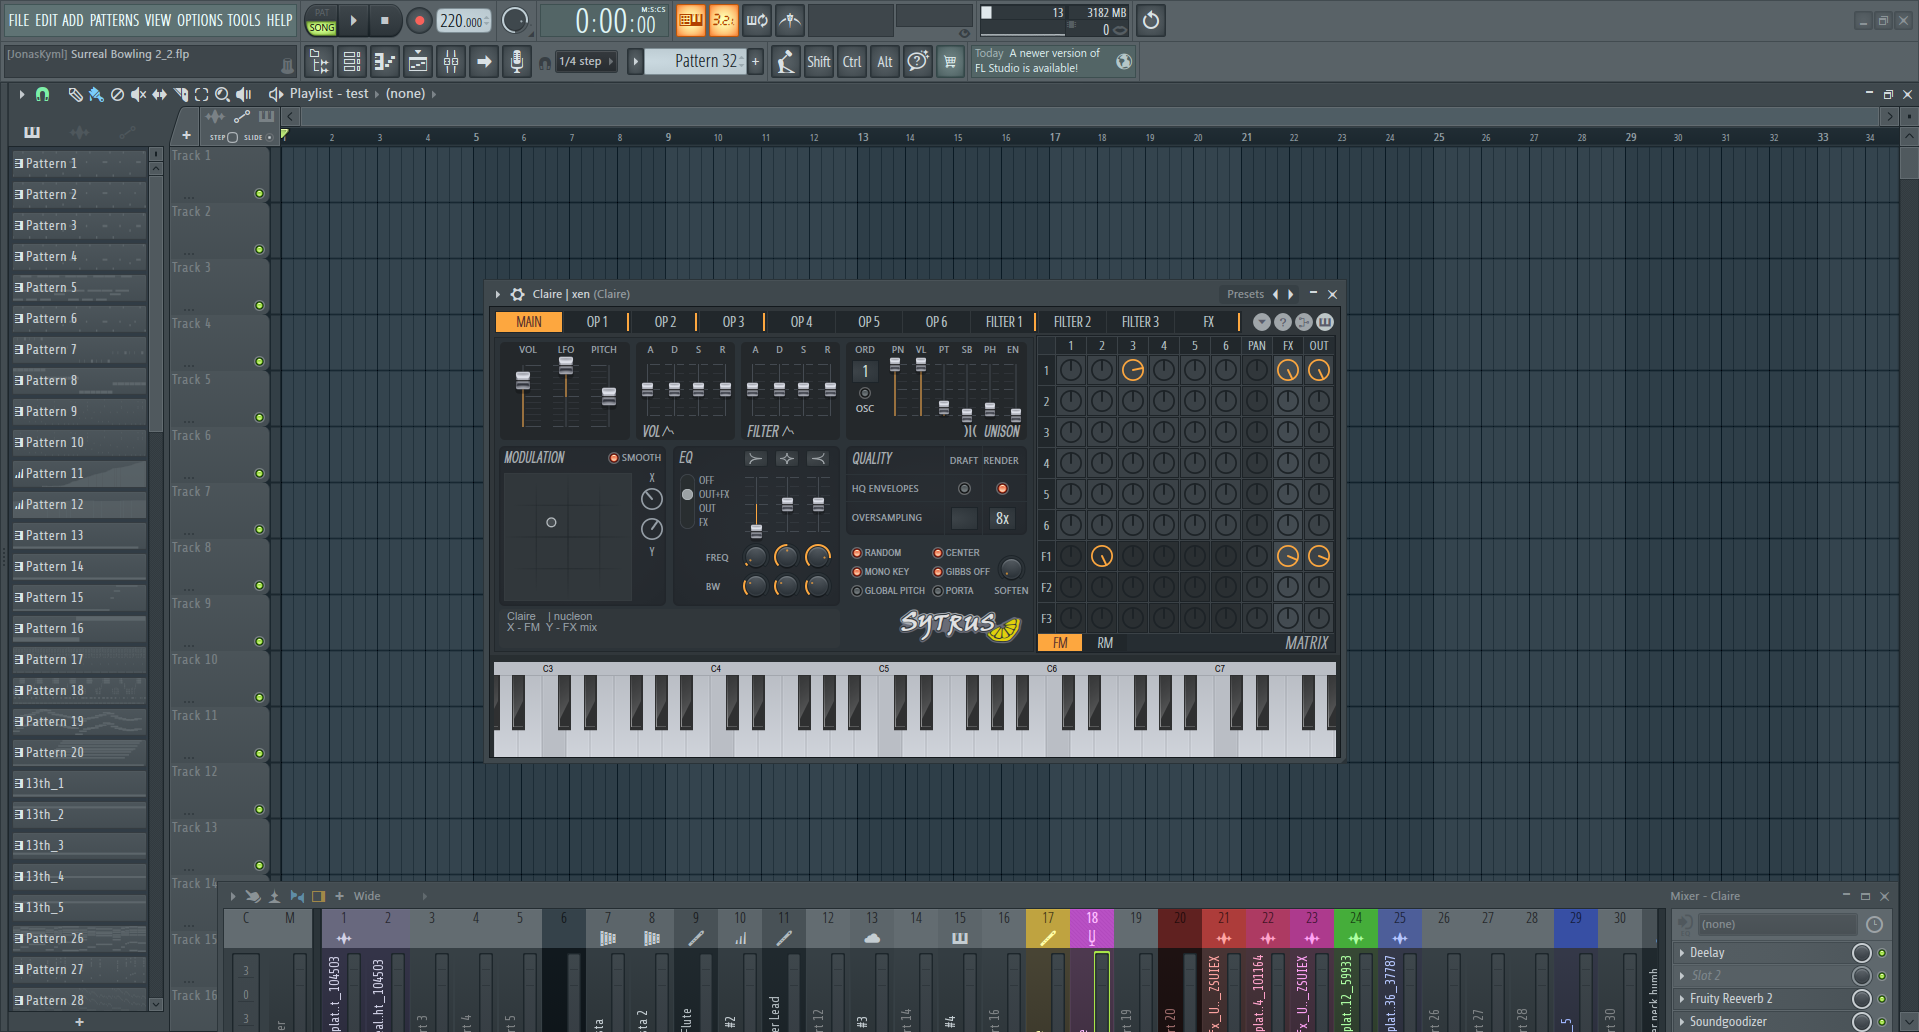
\includegraphics[width=1\textwidth]{img/flstudio/flstudio-sytrus.png}
    \caption{FL Studio -- Sytrus plugin}
    \label{fig:flstudio-sytrus}
\end{figure}

Na obrázku \ref{fig:flstudio-sytrus} je zobrazeno rozhraní Sytrus s několika aktivními operátory a nastavením modulační matice.

\subsubsection{LABs}
LABs je bezplatný plugin od Spitfire Audio, který nabízí rozsáhlou knihovnu realisticky znějících a atmosferických nástrojů. Plugin poskytuje intuitivní ovládání nad základními parametry jako je reverb, hlasitost nebo citlivost, což umožňuje rychle přizpůsobit nástroj požadovanému kontextu bez nutnosti složitého nastavení.

\begin{figure}[h!]
    \centering
    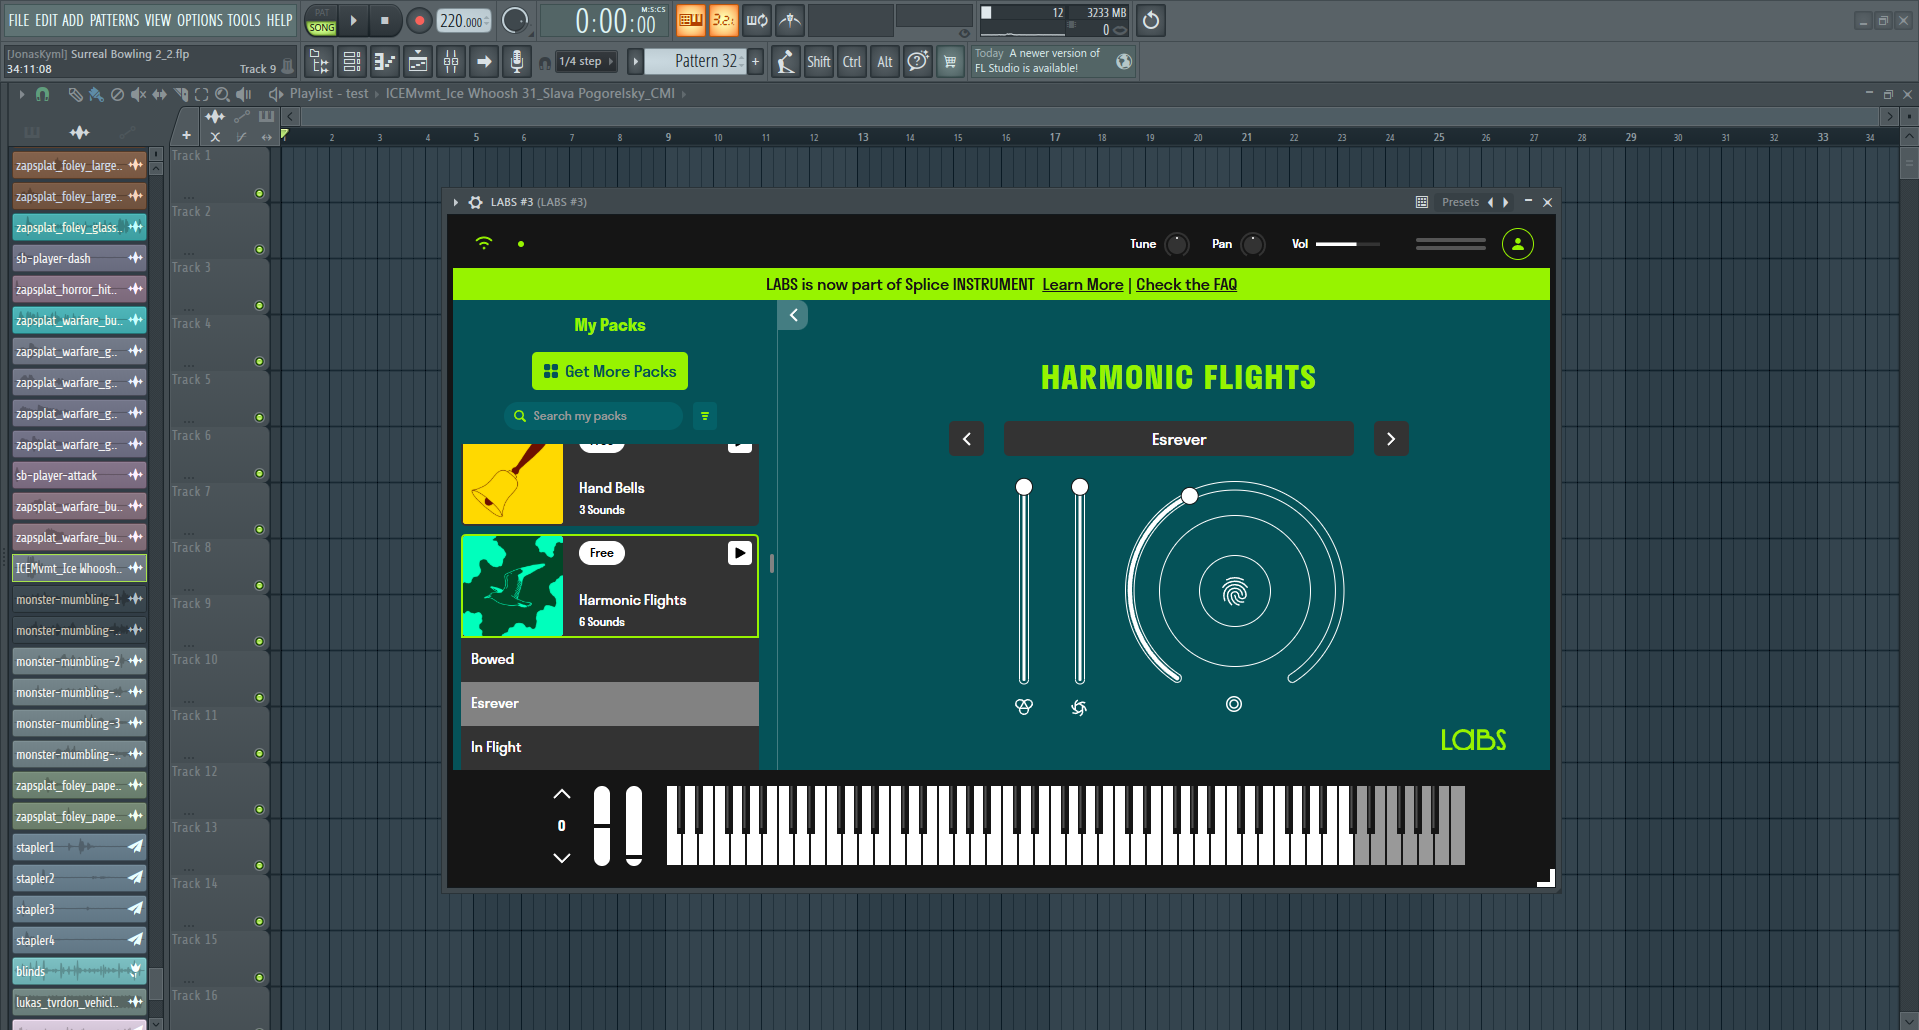
\includegraphics[width=1\textwidth]{img/flstudio/flstudio-labs.png}
    \caption{FL Studio -- LABs plugin}
    \label{fig:flstudio-labs}
\end{figure}

Na obrázku \ref{fig:flstudio-labs} je zobrazeno rozhraní LABs pluginu s několika dostupnými nástroji.

\subsubsection{Deelay}
Deelay je delay plugin, který využívám pro vytváření prostorových echo efektů. Plugin nabízí pokročilé možnosti nastavení oproti běžným delayům -- různé módy filtrace, time/pitch modifikace a synchronizaci na tempo projektu. Speciálně se zaměřuji na využití efektu \emph{Chamber} a tvorbu komplexních, vrstvených delayů, které vytvářejí glitched/corrupted atmosférické zvuky. Tyto techniky přímo korespondují s narativem surrealistické hry, kde zvuková estetika odráží fragmentovanou a deformovanou realitu.

\begin{figure}[h!]
    \centering
    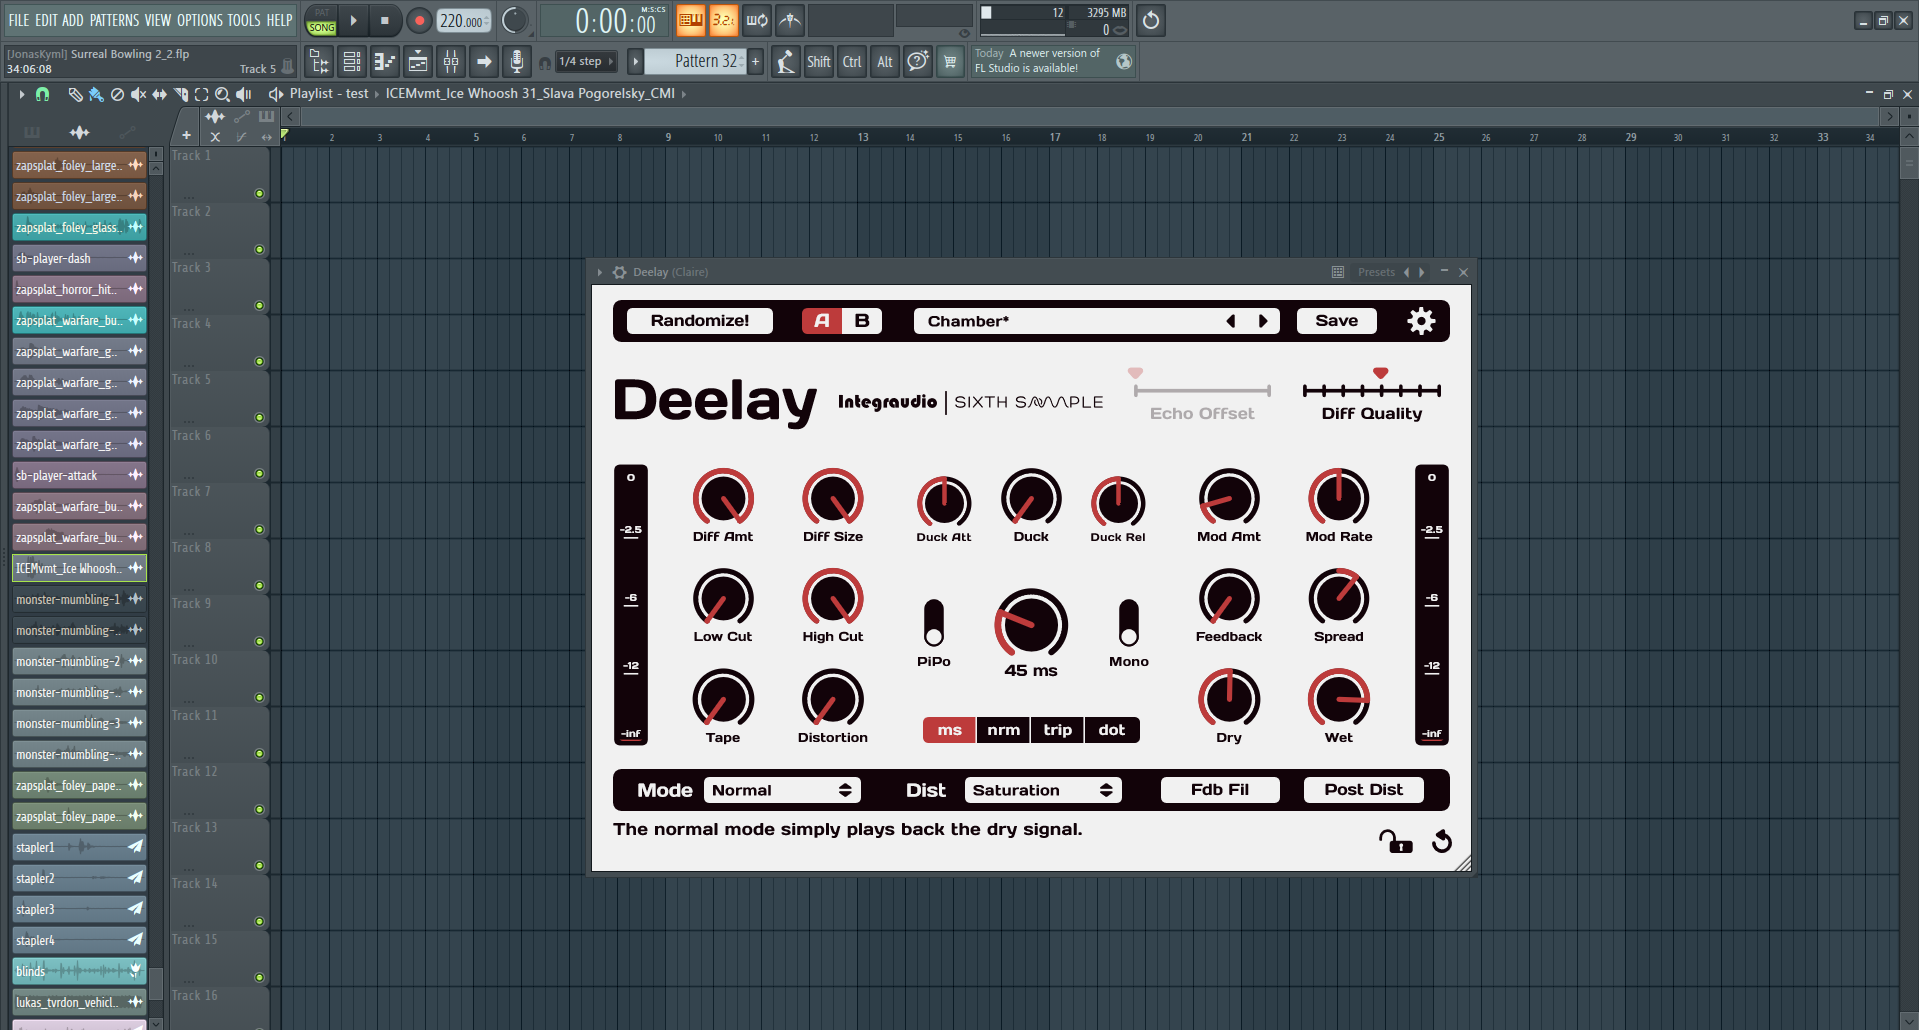
\includegraphics[width=1\textwidth]{img/flstudio/flstudio-deelay.png}
    \caption{FL Studio -- Deelay plugin}
    \label{fig:flstudio-deelay}
\end{figure}

Na obrázku \ref{fig:flstudio-deelay} je zobrazeno rozhraní Deelay pluginu s pokročilými možnostmi nastavení.

\subsubsection{Zvukové efekty -- ZAPSPLAT}
Většina zvukových efektů použitých ve hře pochází z knihovny ZAPSPLAT. Jsem zde Premium Member s aktivním předplatným \emph{Monthly Gold Access}, které mi umožňuje přístup k rozsáhlé databázi profesionálně nahraných zvuků. Tato knihovna pokrývá široké spektrum potřeb -- od prostých UI zvuků až po komplexní prostředí a diegetické efekty.

\begin{figure}[h!]
    \centering
    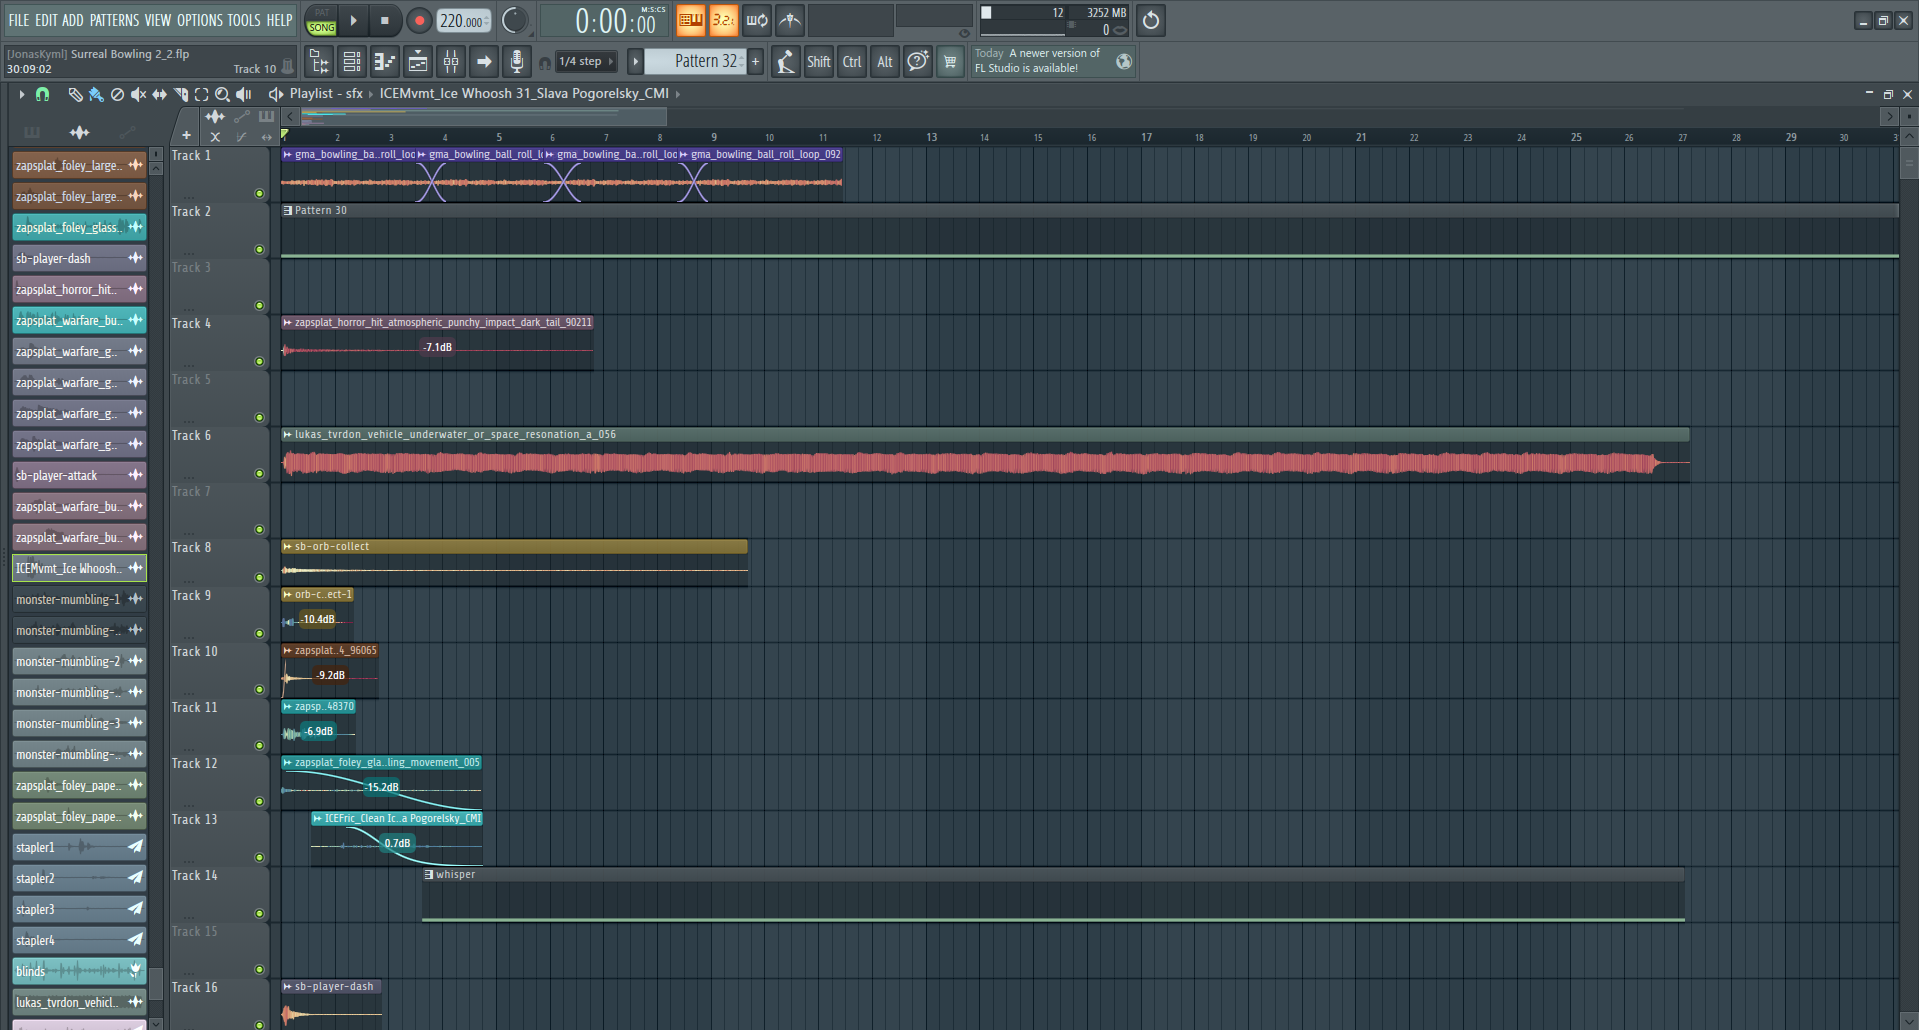
\includegraphics[width=1\textwidth]{img/flstudio/flstudio-sfx.png}
    \caption{FL Studio -- organizace zvukových efektů v jednom arrangements}
    \label{fig:flstudio-sfx}
\end{figure}

Na obrázku \ref{fig:flstudio-sfx} je zobrazena má workflow pro práci se zvukovými efekty. Všechny zvukové efekty mám rozmístěny v jednom dlouhém arrangements, kde každý zvuk zabírá specifickou část časové osy. Při exportu vždy renderuji pouze konkrétní zvuk -- pomocí \emph{Solo} funkce (odmutuje pouze danou stopu) exportuji zvuk do FLAC formátu. Tento přístup mi umožňuje mít rychlý přístup ke všem podobným nebo souvisejícím zvukům na jednom místě a snadno tvořit zvuk celého herního světa. Každý zvuk je tak vždy po ruce a mohu jej kdykoliv upravit či nahradit bez složitého hledání v adresářové struktuře.

\subsubsection{Nativní FL Studio pluginy pro zpracování zvuku}
Kromě externích nástrojů využívám řadu vestavěných (nativních) pluginů FL Studia pro finální zpracování zvuku. Tyto pluginy tvoří základ mého signálového řetězce na jednotlivých Mixer kanálech.

\textbf{Fruity Reverb} je můj primární reverb plugin, který používám jak na nástroje, tak na zvukové efekty. Umožňuje nastavit parametry jako \emph{Room Size}, \emph{Damping}, \emph{Freeze} nebo \emph{Dry/Wet} poměr, díky čemuž lze dosáhnout efektů od malých uzavřených prostorů až po rozsáhlé haly.

\textbf{Destructor} je nástroj původně navržený pro simulaci zkreslení kytarových aparátů, ale jeho potenciál je širší. V mé práci jej používám pro přidání agresivity a textury k syntetickým zvukům nebo pro tvrdší údernost u různých efektů. Plugin nabízí širokou škálu přetížení a harmonického zkreslení, od jemné saturace až po plnohodnotné destruktivní zpracování.

Tato sestava pluginů -- Sytrus a LABs pro generování zvuku, Deelay pro prostorové efekty, následované Destructorem a Fruity Reverb pro další zpracování -- vytváří komplexní, ale přehledný workflow, který mi umožňuje dosahovat profesionálně znějících výsledků.

\subsection{Kategorizace zvuků}
\label{sec:kategorizace-zvuku}

Základní organizace zvukových zdrojů ve hře vychází z klasického dělení na diegetické a nediegetické zvuky. Toto rozdělení určuje nejen jejich umístění v mixovací struktuře, ale také pravidla pro jejich zpracování a implementaci.

\textbf{Diegetické zvuky} jsou ty, které existují uvnitř herního světa -- jsou slyšitelné pro postavy ve hře. Do této kategorie spadá ambience prostředí (kapání v jeskyni, šum vesmíru), zvuky interaktivních objektů (konverzační fragmenty, portál) a zvuky vztahující se k hráči (kroky, skok, útok). Diegetické zvuky typicky využívají prostorové umístění, což znamená, že jejich hlasitost závisí na pozici zdroje vůči hráči.

\textbf{Nediegetické zvuky} existují mimo herní svět -- nejsou součástí příběhu a hráč je slyší pouze jako prostředek komunikace. Patří sem uživatelské rozhraní (kliknutí tlačítek, otevření menu), atmosférické prvky, které nejsou součástí prostředí (například pulzující drone podkres), a samozřejmě hudba.

\subsubsection{Výběr zvukového formátu}
Volba zvukového formátu má přímý dopad na kvalitu i funkčnost zvukového obsahu. Vyzkoušel jsem několik přístupů.

MP3 formát není vhodný pro zvuky, které mají být loopované (opakovaně přehrávané v smyčce). Přestože je MP3 oblíbený pro svou malou velikost, na konec audio souboru vždy přidává metadata, která při loopování vytvářejí nepatrný, ale znatelný klik. Tento zvuk, byť krátký, dokáže zničit atmosféru u jinak plynulé smyčky prostředí.

WAV je můj standardní pracovní formát v FL Studiu. Jelikož nevyužívá žádnou kompresi, \newline zachovává veškerý detail původního zvuku. Pro export do herního projektu se však nehodí kvůli velikosti souborů -- hudební stopy a delší ambience by zabíraly zbytečně mnoho místa.

Experimentoval jsem také s OGG, ale nakonec jsem dospěl k formátu FLAC. Ten nabízí podobnou kvalitu jako WAV, ale umožňuje nastavit vyšší úroveň komprese. Důležité je, že na rozdíl od MP3 formát FLAC na konec souboru nepřidává žádné dodatečné informace, které by při loopování vytvářely klikavé zvuky. FLAC tak představuje ideální kompromis mezi kvalitou, velikostí souborů a spolehlivostí loopování.

\subsection{Hudba}
\label{sec:hudba}

V rámci této verze maturitní práce vznikly tři hudební stopy: \emph{Main Menu Theme}, \emph{Caves -- The Chase} a \emph{Outer Space -- The Chase}. Každá z těchto skladeb plní specifickou roli v celkové zvukové identitě hry.

\subsubsection{Main Menu Theme}
Úvodní skladba main menu je pojata retro stylem, který evokuje éru ragtime hudby z dvacátých let dvacátého století. Hudebně využívá stupnici D Mixolydian, která svým charakteristickým mollovým sedmým stupněm dodává skladbě jazzovou atmosféru. Na celou nahrávku je aplikován efekt \emph{low cut filter}, simulující frekvenční omezení starých audio technologií té doby. Dále je nasimulován charakteristický šum starého vinylového gramofonu. Tyto volby nejsou náhodné -- přímo korespondují s narativem videohry, kde hlavní komunikátor (\emph{The Manager}), bowling alley manažer, promlouvá k hráči (\emph{Pin}) skrze jeho sny pomocí gramofonu. Retro estetika skladby tak vytváří bezprostřední spojení mezi hudební složkou a příběhem.

\subsubsection{Caves -- The Chase}
Tento track patří do úrovně \emph{Caves} a reprezentuje akční pasáže ve stylu \emph{The Chase}. Skladba využívá pětičtvrťový takt (5/4), který svým nepravidelným rytmem vyvolává pocit neznáma a napětí -- posluchač není tolik seznámen s tím, kdy přijde další strong beat. Hlavním nástrojem je krystalická celesta, která svým jasným, zvonivým tónem vytváří kontrast s temným prostředím jeskyní. Hudebně skladba pracuje se stupnicí D\# Phrygian, jež svým sníženým druhým stupněm přidává typický orientální, napjatý charakter. Kromě rytmické linky obsahuje rozsáhlé atmosférické soundscapes s glitch efekty, které budují napětí a evokují nebezpečí blížícího se pronásledujícího Ball.

\subsubsection{Outer Space -- The Chase}
Třetí stopa je koncipována jako sci-fi atmosférický track. Její \emph{arpeggio} linka okamžitě vtahuje posluchače do vesmírného prostředí. Hudebně využívá stupnici G Harmonic Minor. V pozdější části skladby se objevují mikrotonální melodie využívající formát EDO 24 (24 rovnoměrných dělení oktávy), což dále posiluje atmosféru neznáma a surrealismu typickou pro celou hru.

\subsubsection{Plány do budoucna -- leitmotif a struktura alba}
Standardem v herním průmyslu je komponovat hudební stopy s ohledem na jednotlivé postavy, emoce nebo herní situace. Leitmotif je hudební technika, kdy je určitému tématu (postavě, místu, konceptu) přiřazena specifická melodická nebo harmonická fráze, která se vrací v různých obměnách napříč celým dílem. Tím se vytváří silné emocionální a narativní propojení.

V budoucnu plánuji mít pro všech devět levelů dvě hlavní skladby: jednu pro pasáže \emph{The Chase} (akčnější, rytmická, upoutávající pozornost, zdůrazňující rychlé tempo a napětí z útěku před Ball) a jednu pro pasáže \emph{The Exploration} (uklidňující, převážně ambientní, která nevyžaduje pozornost posluchače, ale spíše jej podněcuje k hlubšímu soustředění a zamyšlení). Kromě toho budou vytvořeny specifické skladby pro důležité momenty a postavy. V tomto kontextu začíná hrát leitmotif klíčovou roli -- \emph{The Manager}, \emph{The Ball} i další prvky si postupně vybudují své vlastní hudební identity, které se budou vracet napříč celým albem.

\section{Post-processing hry}
\label{sec:post-processing-hry}

Post-processing je klíčovou součástí moderního vizuálního stylu videohry, jelikož dokáže \newline transformovat i jednoduchou grafiku v něco vizuálně působivého. V rámci \emph{Surreal Bowling: Salvation Path} využívám Unity Universal Render Pipeline (URP), která poskytuje výkonný a flexibilní systém pro aplikaci grafických efektů.


\subsection{Global Volume}
\label{sec:global-volume}

V URP je centrem veškerého post-processingu objekt \emph{Global Volume}. Ten funguje jako kontejner, který sdružuje všechny efekty a aplikuje je na celou scénu. V hierarchii Unity je tento objekt typicky umístěn jako samostatný \texttt{GameObject} s připojenou komponentou \texttt{Volume}, která obsahuje seznam jednotlivých \emph{Volume Overrides} -- tedy konkrétních efektů, které mají být aplikovány.

Global Volume je nakonfigurován tak, aby pokrýval celou herní plochu (\emph{Global} režim) a byl perzistentní mezi scénami, což zajišťuje konzistentní vizuální styl bez nutnosti znovu nastavovat efekty při přechodu mezi úrovněmi. V editoru je toto nastavení zobrazeno na obrázku \ref{fig:unity-global-volume}.

\begin{figure}[h!]
    \centering
    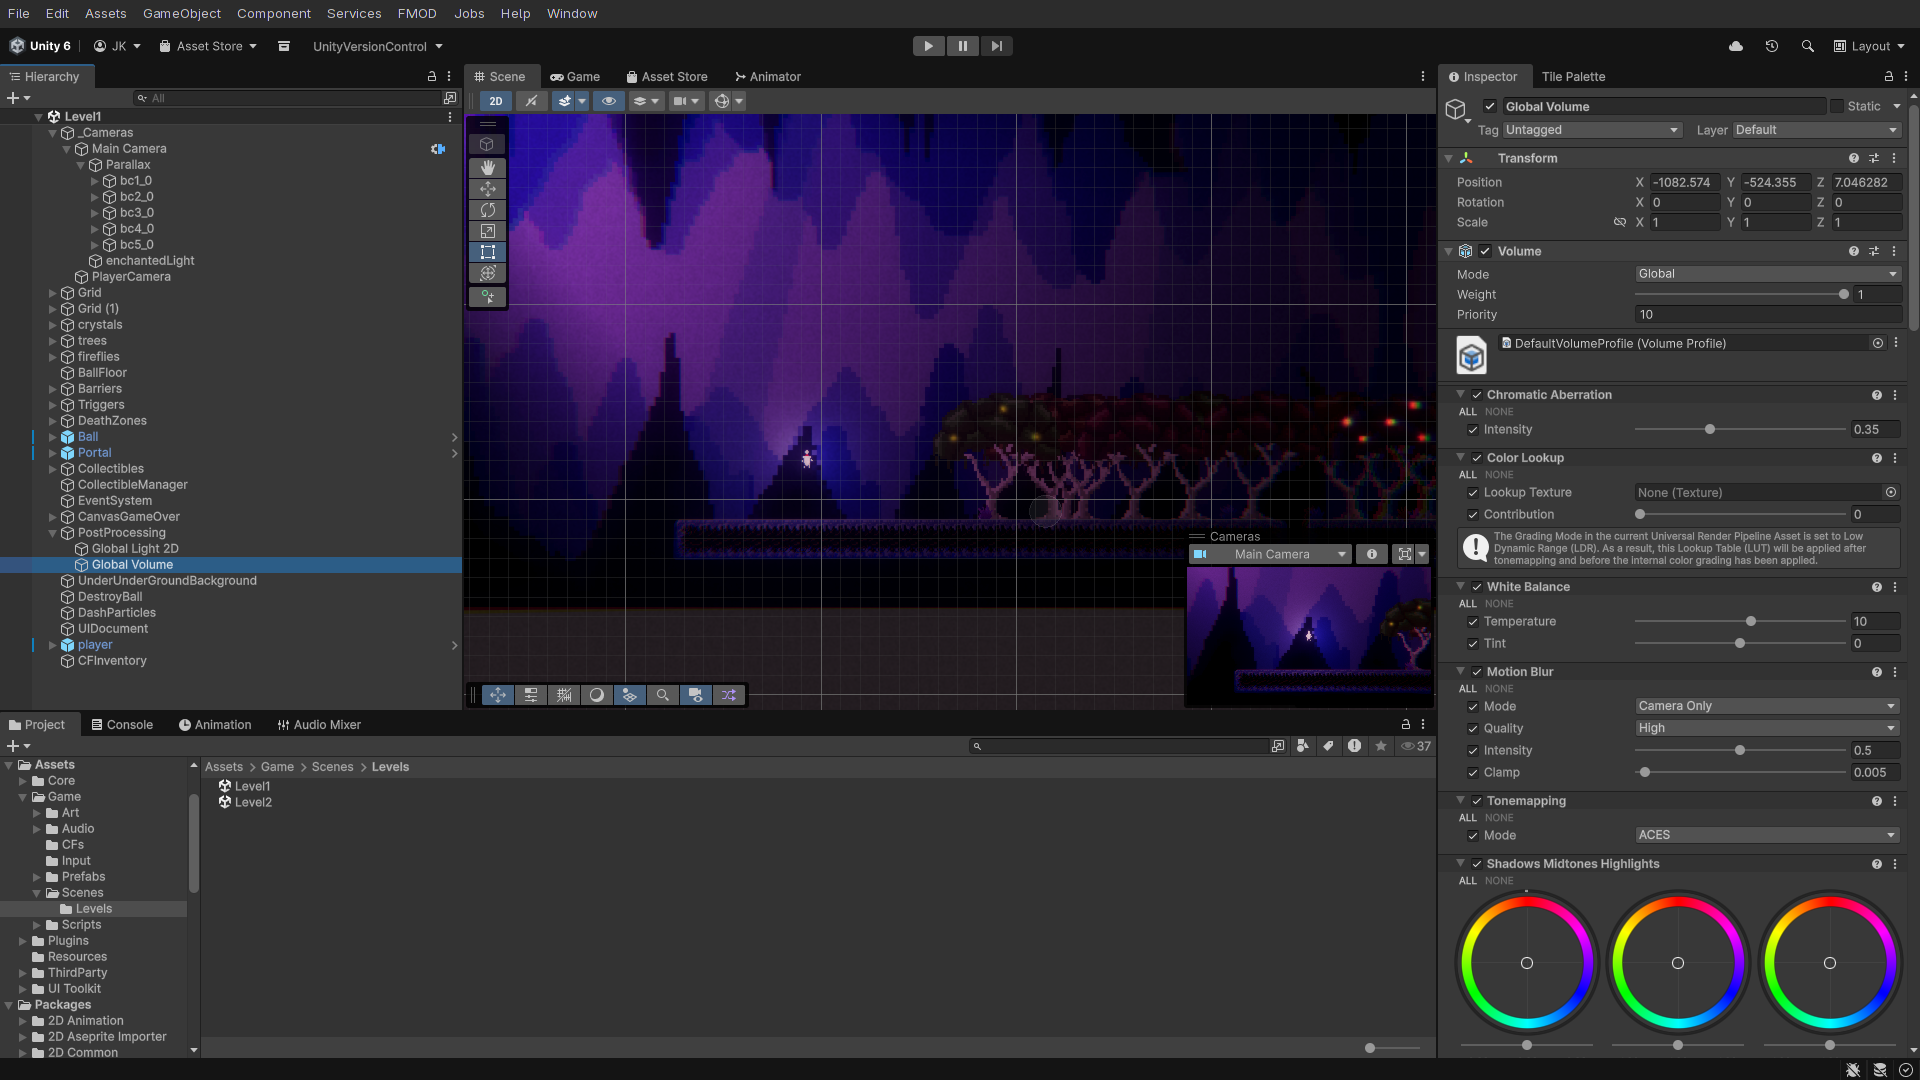
\includegraphics[width=0.8\textwidth]{img/unity/unity-global-volume.png}
    \caption{Global Volume v Unity Editoru}
    \label{fig:unity-global-volume}
\end{figure}

Každý efekt v rámci Global Volume má svou prioritu a intenzitu. Priorita určuje pořadí aplikace efektů, zatímco intenzita umožňuje jemné doladění -- například plný bloom může být příliš agresivní, a proto jej nastavuji na 60\% intenzitu.

\subsection{Použité efekty, jejich nastavení a bindnutí do kódu}
\label{sec:pouzite-efekty}

V rámci post-processingu využívám několik specifických efektů, které dohromady vytvářejí charakteristický vizuální styl hry.

\subsubsection{Bloom}
Bloom je jeden z nejdůležitějších efektů pro celkovou vizuální kvalitu hry. Princip spočívá v tom, že jasné části obrazu prosakují do okolních pixelů, čímž vzniká charakteristické záření kolem světelných zdrojů. V kontextu hry bloom zdůrazňuje světlušky v korunách stromů, collectible objekty i světelný efekt kolem hráče. Toto nastavení je dostatečně výrazné, aby hra působila vizuálně zajímavě, ale ne natolik agresivní, aby rušilo herní mechaniky.

Bloom je součástí defaultního URP assetu a nevyžaduje žádné bindování do kódu -- je aktivní trvale přes Global Volume.

\subsubsection{Chromatic Aberration}
Chromatic aberration (chromatická vada) způsobuje rozklad barev na okrajích obrazovky, kde se jednotlivé barevné kanály (červená, zelená, modrá) mírně posouvají. Tento efekt je tradičně považován za nedostatky optiky, ale v herním designu se využívá pro vytvoření specifické atmosféry.

V \emph{Surreal Bowling: Salvation Path} slouží chromatic aberration k navození snivého, surrealistického pocitu, který odpovídá celkovému tématu hry. Podobně jako bloom, i tento efekt je aktivní trvale přes Global Volume a není manipulován v žádném kódu.

\begin{figure}[h!]
    \centering
    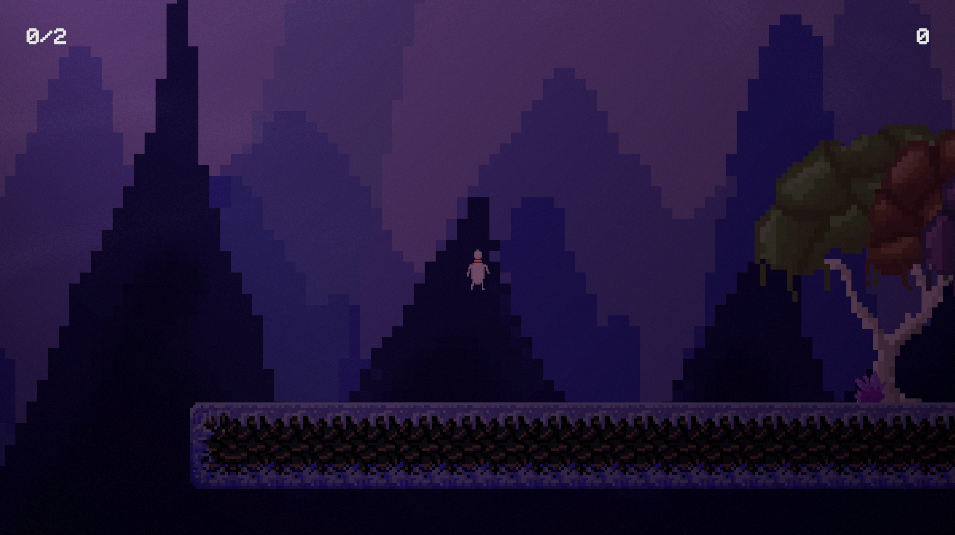
\includegraphics[width=0.45\textwidth]{img/unity/unity-postprocessing-off.png}
    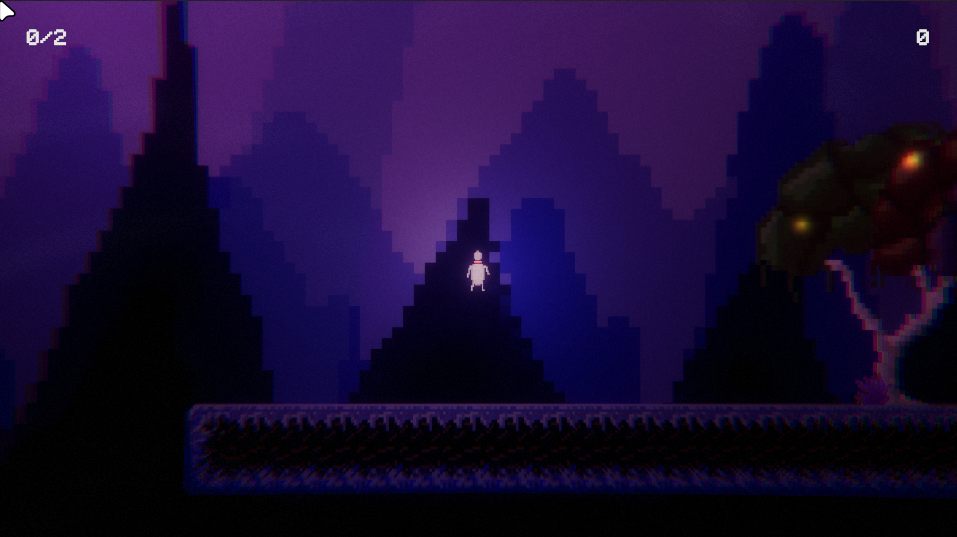
\includegraphics[width=0.45\textwidth]{img/unity/unity-postprocessing-on.png}
    \caption{Ukázka vlevo bez post-processingu, vpravo s post-processingem}
    \label{fig:unity-postprocessing}
\end{figure}

Na obrázku \ref{fig:unity-postprocessing} je vidět zásadní rozdíl, který post-processing a osvětlení přináší. Levý obrázek ukazuje scénu tak, jak by vypadala bez jakýchkoliv vizuálních efektů -- tmavší, plochá, bez atmosféry. Pravý obrázek pak ukazuje tutéž scénu s aplikovaným post-processingem a Light 2D systémem -- prostředí získává hloubku, atmosféru a vizuální zajímavost.

Velmi mírný motion blur je využit pro zjemnění rychlých pohybů kamery a hráče. Na rozdíl od filmového motion blur, který může být velmi výrazný, je zde nastaven na minimální úroveň, aby nepůsobil rušivě, ale přesto přidal určitou dynamiku.

Color adjustments jsou klíčové pro celkovou atmosféru hry. Nejdůležitějším parametrem je \emph{Post Exposure}, který je nastaven na hodnotu 0.5. Tím se celkový jas sníží, což vytváří temnější prostředí odpovídající atmosféře hry. Toto nastavení je rovněž součástí Global Volume a je aktivní trvale.

%\subsection{Death Screen -- DeathEffect.cs}
%\subsubsection{DeathEffect.cs}
Komponenta \texttt{DeathEffect.cs} je skript, který dynamicky manipuluje s post-processing parametry při úmrtí hráče. Jak již bylo zmíněno v podkapitole \ref{sec:ostatni-efekty-vfx}, tento skript ovlivňuje proměnné \texttt{Volume} profilu.

\begin{lstlisting}[caption={DeathEffect.cs -- základní struktura}, label={lst:deatheffect}]
using UnityEngine;
using UnityEngine.Rendering;
using UnityEngine.Rendering.Universal;

public class DeathEffect : MonoBehaviour
{
    private Volume volume;
    private ColorAdjustments colorAdjustments;
    
    [SerializeField] private float targetExposure = -2f;
    [SerializeField] private float transitionSpeed = 2f;
    
    private void Start()
    {
        volume = GetComponent<Volume>();
        volume.profile.TryGet(out colorAdjustments);
    }
    
    private void Update()
    {
        if (colorAdjustments != null)
        {
            float currentExposure = colorAdjustments.postExposure.value;
            float newExposure = Mathf.Lerp(currentExposure, targetExposure, Time.deltaTime * transitionSpeed);
            colorAdjustments.postExposure.value = newExposure;
        }
    }
}
\end{lstlisting}

V aktuální implementaci skript snižuje post-exposure při úmrtí hráče, čímž vytváří tmavý, cinematický efekt -- obraz postupně ztmavne, dokud není hráč respawnován. Po respawnu se hodnota post-exposure vrací zpět na výchozí 0.5.

Tento efekt je aktivován v momentě, kdy hráč vstoupí do \texttt{DeathZone} triggeru. Skript \texttt{PlayerDeath.cs} detekuje kolizi a aktivuje \texttt{DeathEffect} komponentu, která následně ovlivňuje post-processing parametry.

\begin{lstlisting}[caption={PlayerDeath.cs -- aktivace Death Effectu}, label={lst:playerdeath-deatheffect}]
private void OnTriggerEnter2D(Collider2D collision)
{
    if (collision.CompareTag("DeathZone"))
    {
        ActivateDeathEffect();
    }
}

private void ActivateDeathEffect()
{
    DeathEffect deathEffect = FindFirstObjectByType<DeathEffect>();
    if (deathEffect != null)
    {
        deathEffect.TriggerDeathEffect();
    }
}
\end{lstlisting}

Kromě snižování exposure může \texttt{DeathEffect.cs} v budoucnu ovlivňovat i saturaci (snížení na 0 pro černobílý efekt) a přidávat vinceetting (tmavé rohy obrazovky), čímž se ještě více zdůrazní cinematický charakter úmrtí.

\subsection{Vizuální styl hry}
\label{sec:vizualni-styl-hry}

Vizuální styl \emph{Surreal Bowling: Salvation Path} je záměrně navržen tak, aby vyvolával pocit snu, surrealismu a melancholie. Kombinace výše zmíněných post-processing efektů vytváří jedinečnou atmosféru, která hru odlišuje od začátečnických indie herních projektů a blíží se profesionálním designovým standardům.

Temný prostředí (díky post-exposure -0.5) vytváří pocit nebezpečí a tajemna. Hráč se pohybuje v temném prostředí, což podporuje explorativní herní mechaniky \emph{The Exploration} pasáží.

Chromatic aberration a mírný bloom dodávají hře surreální vzhled. Hranice mezi světem hry a snem se rozmazávají, což odpovídá celkovému příběhu o hledání cesty ke spasení.

V budoucnu je plánováno rozšíření vizuálního stylu o další prvky:
\begin{itemize}
    \item \textbf{Vignette} -- tmavé rohy obrazovky, které ještě více zdůrazní cinematický vzhled
    \item \textbf{Film Grain} -- jemný šum, který přidá na textuře a retro pocitu
    \item \textbf{Další color grading} -- specifické barevné korekce pro různé části hry (jiné barvy pro \emph{The Chase} pasáže, jiné pro \emph{The Exploration})
\end{itemize}

Celkově post-processing hraje klíčovou roli v tom, jak hráč vnímá herní svět. Bez něj by grafika byla pouze funkční -- s ním se stává profesionálnějším výrazem.
\chapter{Závěr}
\label{sec:zaver}

Tento projekt představuje výsledek mé dlouhodobé práce na \emph{Surreal Bowling: Salvation Path}, který vznikl v rámci tří spolupracujících maturitních prací.

Během tvorby této práce se mi podařilo vytvořit komplexní audiovizuální systém pro 2D videohru, který zahrnuje pokročilé vizuální efekty pomocí Unity Universal Render Pipeline, profesionální zvukový design prostřednictvím FMOD Studio a vlastní hudbu v FL Studio, a moderní uživatelské rozhraní založené na UI Toolkitu. Práce mi umožnila prohloubit mé zkušenosti s implementací audia do herního kódu a efektivně propojit audio systém s herními mechanikami.

Mezi dovednosti, které jsem během práce rozvinul, patří práce s globálními objekty v Unity, správa zvukového mixu ve FMOD Studiu, tvorba hudebních kompozic v FL Studio a efektivní komunikace v týmu. FL Studio jsem používal již před touto prací, ale tato práce mi umožnila využít tyto dovednosti v profesionálnějším kontextu a propojit je s herním vývojem.

Spolupráce v týmu Still Thinking Studio byla klíčovým prvkem celého projektu. Naše týmová spolupráce se mohla díky této práci ověřit v praxi -- naučili jsme se efektivně komunikovat nápady, spolupracovat na společných cílech a respektovat role jednotlivých členů. Zkušenost s koordinací tří maturitních prací na jednom projektu nám ukázala, jak důležitá je kvalitní komunikace pro úspěšný herní projekt.

Je důležité zmínit, že projekt \emph{Surreal Bowling: Salvation Path} vznikl na game jamu od Game Devs Ostrava, kde jsme z 12 týmů zvítězili na prvním místě. Od té doby jsme se účastnili dalších soutěží a konferencí. Tato maturitní práce tedy není prvním krokem naší cesty, ale spíše příležitostí, jak na našem projektu dále pracovat a rozvíjet ho.

V současnosti se náš tým připravuje na účast na konferenci \emph{Game Access Conference '26} v Brně, kde budeme prezentovat nejen \emph{Surreal Bowling: Salvation Path}, ale také náš druhý projekt \emph{Dissonantia} -- top-down view roguelike hru. Tato konference představuje významný milník v naší developerské dráze a příležitost získat zpětnou vazbu od profesionálů v oboru.

Do budoucna plánujeme pokračovat ve vývoji obou her s cílem je vydat na platformě Steam. Věříme, že kvalita naší práce může zaujmout hráče a potenciálně i sponzory nebo vydavatele, kteří by mohli podpořit další rozvoj našich projektů.

Celkově tato práce ověřila naše schopnosti vyvíjet hry a díky příležitosti od naší školy jsme mohli pokračovat v práci na vlastním projektu. Získané zkušenosti budou cenným základem pro naši budoucnost v herním průmyslu.

\listoffigures

\printbibliography

\end{document}